\chapter{Efficiency of lepton trigger, reconstruction, and identification}
\label{chap:efficiency}
%\autoref{chap:efficiency}
After reconstructing leptons in CMS using the information from the detector subsystems,
further offline requirements are applied for the purpose of high quality and low background lepton identification.
The choice of these requirements depends on the analysis, and several well-defined working points are optimized
and released by the relevant Physics Object Groups. The figure of merit for lepton identification is the efficiency,
and the various working points are usually described qualitatively in terms of ``tightness,''
with a tighter selection corresponding to lower efficiency and higher purity.
In this note we refer to the whole slew of offline requirements applied to reconstructed leptons under the umbrella term of identification, including quantities such as relative isolation.

Previously, at lower center-of-mass energies, resonant leptonic decays of the $J/\psi$ meson were used to measure lepton identification efficiency.
In Run II at the LHC, we make use of the large cross section of the Z boson resonance and observe its leptonic decays to extract the lepton efficiencies for a wide range of lepton energies and rapidity;
while the $J/\psi$ meson is also still used for efficiency studies at lower transverse momentum.
This chapter describes how the efficiency is measured in data and simulation by studying dilepton events with invariant mass close to the Z boson resonance peak at 91.1876 $\GeV$.
The ensuing discussion presents results for the ``Medium 2016'' cut-based identification algorithm.

\section{Event selections for the tag-and-probe method}
\label{sec:tnpsel}
The so-called ``tag-and-probe'' selection consists of a high purity $\dyll$ selection with a
well-identified tag lepton and an oppositre sign probe.
The tag electron (muon) must pass the tight identification, have transverse momentum greater than 30 (25) $\GeV$, 
have $\abs{\eta}<$ 2.5 (2.4), and be matched to the leptonic trigger firing.
The probe electron must have transverse momentum greater than 10 $\GeV$ and $\abs{\eta}<$ 2.5.
For the probe muons, we consider a collection of general tracks. These tracks must have transverse momentum 
greater than 10 $\GeV$, $\abs{\eta}<$ 2.4, and a vertex whose longitudinal position is within 4 cm of that of the tag.

The selection also includes a truth-matching procedure when applied to simulated Drell-Yan samples,
so that all simulated reconstructed dileptons come from leptonic Z decays.
The reconstructed leptons must each have a small angular separation $\Delta R = \sqrt{ \Delta\phi^{2} + \Delta\eta^{2} }$ 
less than 0.3 with a final-state lepton of the same flavor at generator level. For muons, the generator-level and reconstructed
transverse momenta must also be compatible within 10\%.

\subsection{Probe multiplicity calculation}
In order to increase the signal purity of the muon selection, we perform a probe multiplicity calculation to
remove combinatorial background. The track collection as described above is considered, albeit with a 
lowered transverse momentum cut of 3 $\GeV$. Then, the number of opposite sign tag-track pairs having invariant mass above
60 $\GeV$ is counted for each tag; this gives the probe multiplicity. Any muon tags having probe multiplicity
greater than 1 are not considered in the ensuing tag and probe analysis.

\section{Control samples for the lepton efficiencies}
Two independent data samples are chosen to faithfully represent the background distributions for the
tag-and-probe fitting methods. They are defined below.
\label{sec:tnpcontrol}

\subsection{Lepton pion selection}
The mass spectrum of the combinatorial background in the Z selection can be modeled well by selecting
essentially random pairs of tag leptons and charged hadrons whose invariant mass falls within the relevant window.
We select a tag electron (muon) exactly the same as before, along with a PF charged hadron having $\pt>10~\GeV$ and $\abs{\eta}<2.5$
which must originate from the primary event vertex.

The charged hadrons selected in such a way are predominantly but not exclusively pions.
As the CMS detector does not have charged hadron particle ID capabilities beyond $\frac{dE}{dx}$,
which is ineffective for such boosted particles, we have little way of knowing if they are really pions
instead of kaons, protons, or something even more charming.
Thus, we refer to them somewhat ignorantly using $\pi^{\pm}$ as shorthand.

To obtain a data sample orthogonal to the Z selection, and to suppress contamination by Z events,
we remove events from the \ensuremath{\ell^{\pm}\pi^{\pm}} selection with the following cuts:
\begin{itemize}
\item Reject events containing a tag electron (muon) and another reconstructed electron (muon)
\item Reject \ensuremath{\pi^{\pm}} probes with separation $\Delta R$ less than 0.3 with any reconstructed electron or muon
\item Require the same charge assignment for the tag lepton and the pion probe
\end{itemize}

Furthermore, due to low event yields in this selection at higher probe energies for the electron case,
we use an $\eta$-inclusive form of this selection to build the shapes that are used in each bin of probe $\eta$ for probes with $p_{T} > 50~\GeV$.

The \ensuremath{\ell^{\pm}\pi^{\pm}} selection is effective at modeling the background combinatorics, largely
arising from QCD and the W+jets process. However, it fails to accurately
model the lower energy contribution from the non-resonant background processes e.g. $\ttbar \to 2\ell 2\nu 2b$ and $\dytt$.
\subsection{Electron muon selection}
The Z(ee) background can also be modeled by selecting a muon tag along with an electron probe.
In this case, we choose tags from the muons passing tight identification, with kinematic cuts the same as the electron tags,
but the probes are chosen as in the Z(ee) selection. The opposite sign charge requirement is dropped. 
As with the \ensuremath{\ell^{\pm}\pi^{\pm}} selection, we also use an $\eta$-inclusive selection for the \ensuremath{e\mu}-derived shape at probe $p_{T} > 50~\GeV$.
The shape obtained this way is effective for lower energy electrons, but does not accurately model the electron tag kinematics nor the lepton fake rate at higher energies.

Thus, the most effective data-driven background shape for the Z(ee) selection was determined to be a linear combination of
the \ensuremath{\ell^{\pm}\pi^{\pm}} and \ensuremath{e\mu} selections, with the relative contribution a floating parameter.
This allows the efficiency extraction procedure to empirically determine what would otherwise be a
complicated expression of the lepton fake rates, the lepton efficiencies, 
the cross-sections of contributing background processes, and numerous other factors.

Figure~\ref{fig:ZeeEPiEMu} shows how the true background shape is approximated using this linear combination of the two data-driven shapes.

\begin{figure}
	\centering
	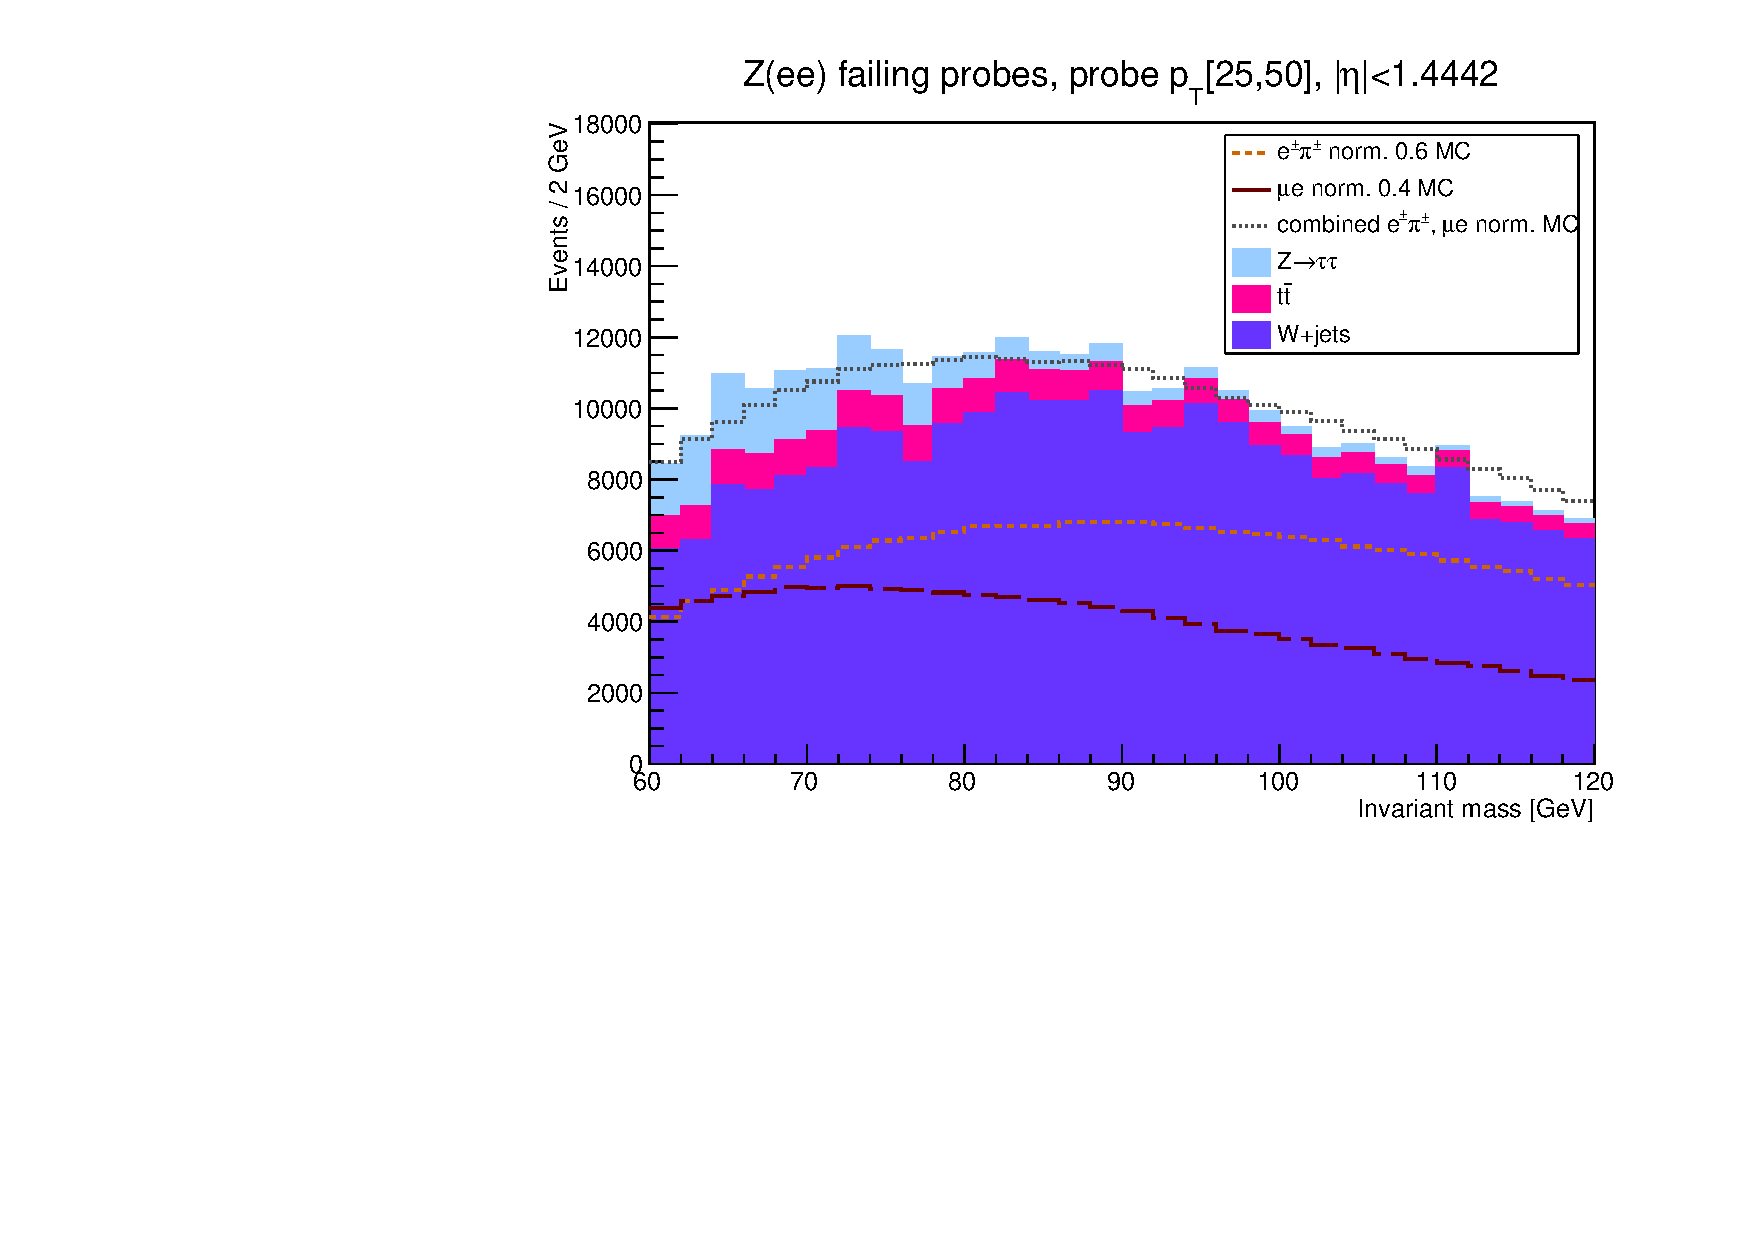
\includegraphics[width=0.75\textwidth]{figures/ZeeEPiEMu.pdf}
	\caption{Simulation of the true background shape, compared with the shapes of the \ensuremath{\ell^{\pm}\pi^{\pm}} selection, the \ensuremath{e\mu} selection, and a linear combination of the two.
    The background is normalized to the integrated luminosity of the 2016 dataset.}
	\label{fig:ZeeEPiEMu}
\end{figure}
\section{Fitting techniques}
\label{sec:tnpfits}
The data efficiency is determined by performing a combined signal plus background fit to each of the
passing and failing categories, in each of the bins of kinematic phase space. 
The efficiency extraction fit provides the number of signal Z events in the passing and failing categories 
by measuring the relative contribution of signal and background.
The nominal values for the signal and background yields in data are fit using a signal hypothesis
of truth-matched Drell-Yan Monte Carlo templates (as described in Section~\ref{sec:tnpsel}),
convoluted with a Gaussian resolution function which allows for widening and shifting of the
simulated peak position. The background hypothesis is a fixed shape derived from data, as
described in Section~\ref{sec:tnpcontrol}.
In the dielectron fits, the relative contribution of \ensuremath{e^{\pm}\pi^{\pm}} versus 
{\ensuremath{e\mu} data is a free parameter in the fit.

The binning choice for the probe leptons is the following:
\begin{itemize}
\item Probe electron $\pt$: $\{$10, 15, 20, 25, 30, 35, 40, 42, 44, 46, 48, 50, 55, 60, 70, 100$\}$ $\GeV$;
\item Probe electron $\eta$: $\{$-2.5, -2.4, -2.3, -2.2, -2.1, -2.0, -1.8, -1.566, -1.4442, -1.2, -1, -0.8, -0.6, -0.4, -0.2, 0, 0.2, 0.4, 0.6, 0.8, 1, 1.2, 1.4442, 1.566, 1.8, 2.0, 2.1, 2.2, 2.3, 2.4, 2.5$\}$;
\item Probe muon $\pt$: $\{$10, 15, 20, 25, 30, 35, 40, 45, 50, 55, 60, 120$\}$ $\GeV$;
\item Probe muon $\eta$: $\{$-2.4, -2.1, -1.6, -1.2, -0.9, -0.3, -0.2, 0.2, 0.3, 0.9, 1.2, 1.6, 2.1, 2.4$\}$;
\end{itemize}

Representing the phase space bin and the pass/fail category with the index $i$,
the number of signal events $N_{sig}^{i}$ (and associated statistical uncertainty) in this bin
is calculated as the total number of data events $N_{total}^{i}$ (Poisson distributed),
minus the estimated background yield $N_{bkg}^{i}$
(with statistical uncertainty from the negative likelihood minimization procedure).
Then, in each phase space bin, the efficiency is determined as
\begin{equation}
  \varepsilon = \frac{N_{\mathrm{Signal}}^{\mathrm{pass}}}{N_{\mathrm{Signal}}^{\mathrm{pass}}+N_{\mathrm{Signal}}^{\mathrm{fail}}}
\end{equation}
and the statistical errors are propagated conservatively assuming zero, not negative
correlation between the passing and failing signal yields.

Examples of the nominal efficiency extraction fits for dimuons are shown in Figures~\ref{fig:ZmmNominalFits1} and~\ref{fig:ZmmNominalFits2}.
Similar examples for dielectrons are shown in Figures~\ref{fig:ZeeNominalFits1} and~\ref{fig:ZeeNominalFits2}.
In order to assess the goodness-of-fit, we compute a modified $\chi^2$ test which accounts for
statistical uncertainties in the data as well as the MC signal template, as shown in the plots.

The MC efficiency is determined by counting the normalized yields of the passing and failing templates described above.
\begin{figure}
\centering
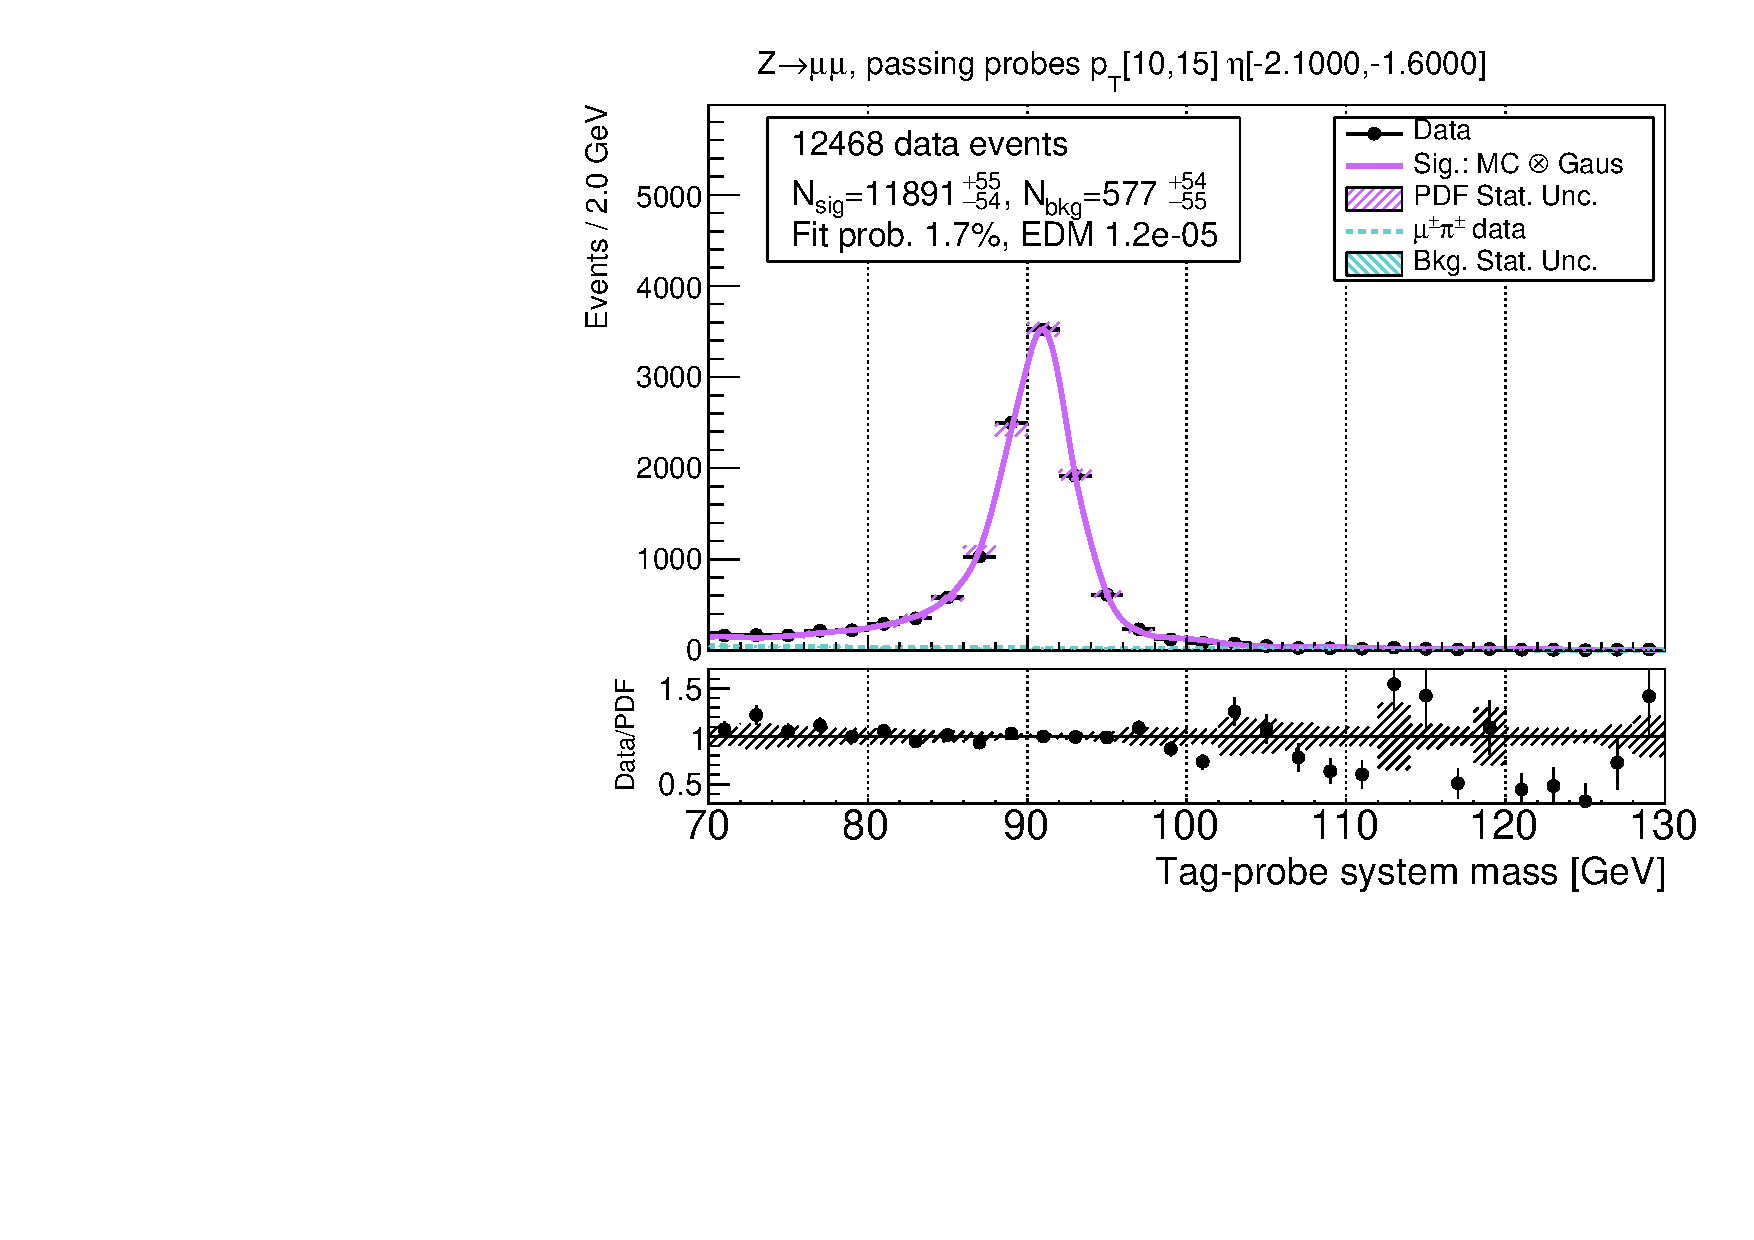
\includegraphics[width=0.49\textwidth]{figures/Zmm_RecoTemplate_BkgLPi_pass_ptBin0_etaBin1.pdf}
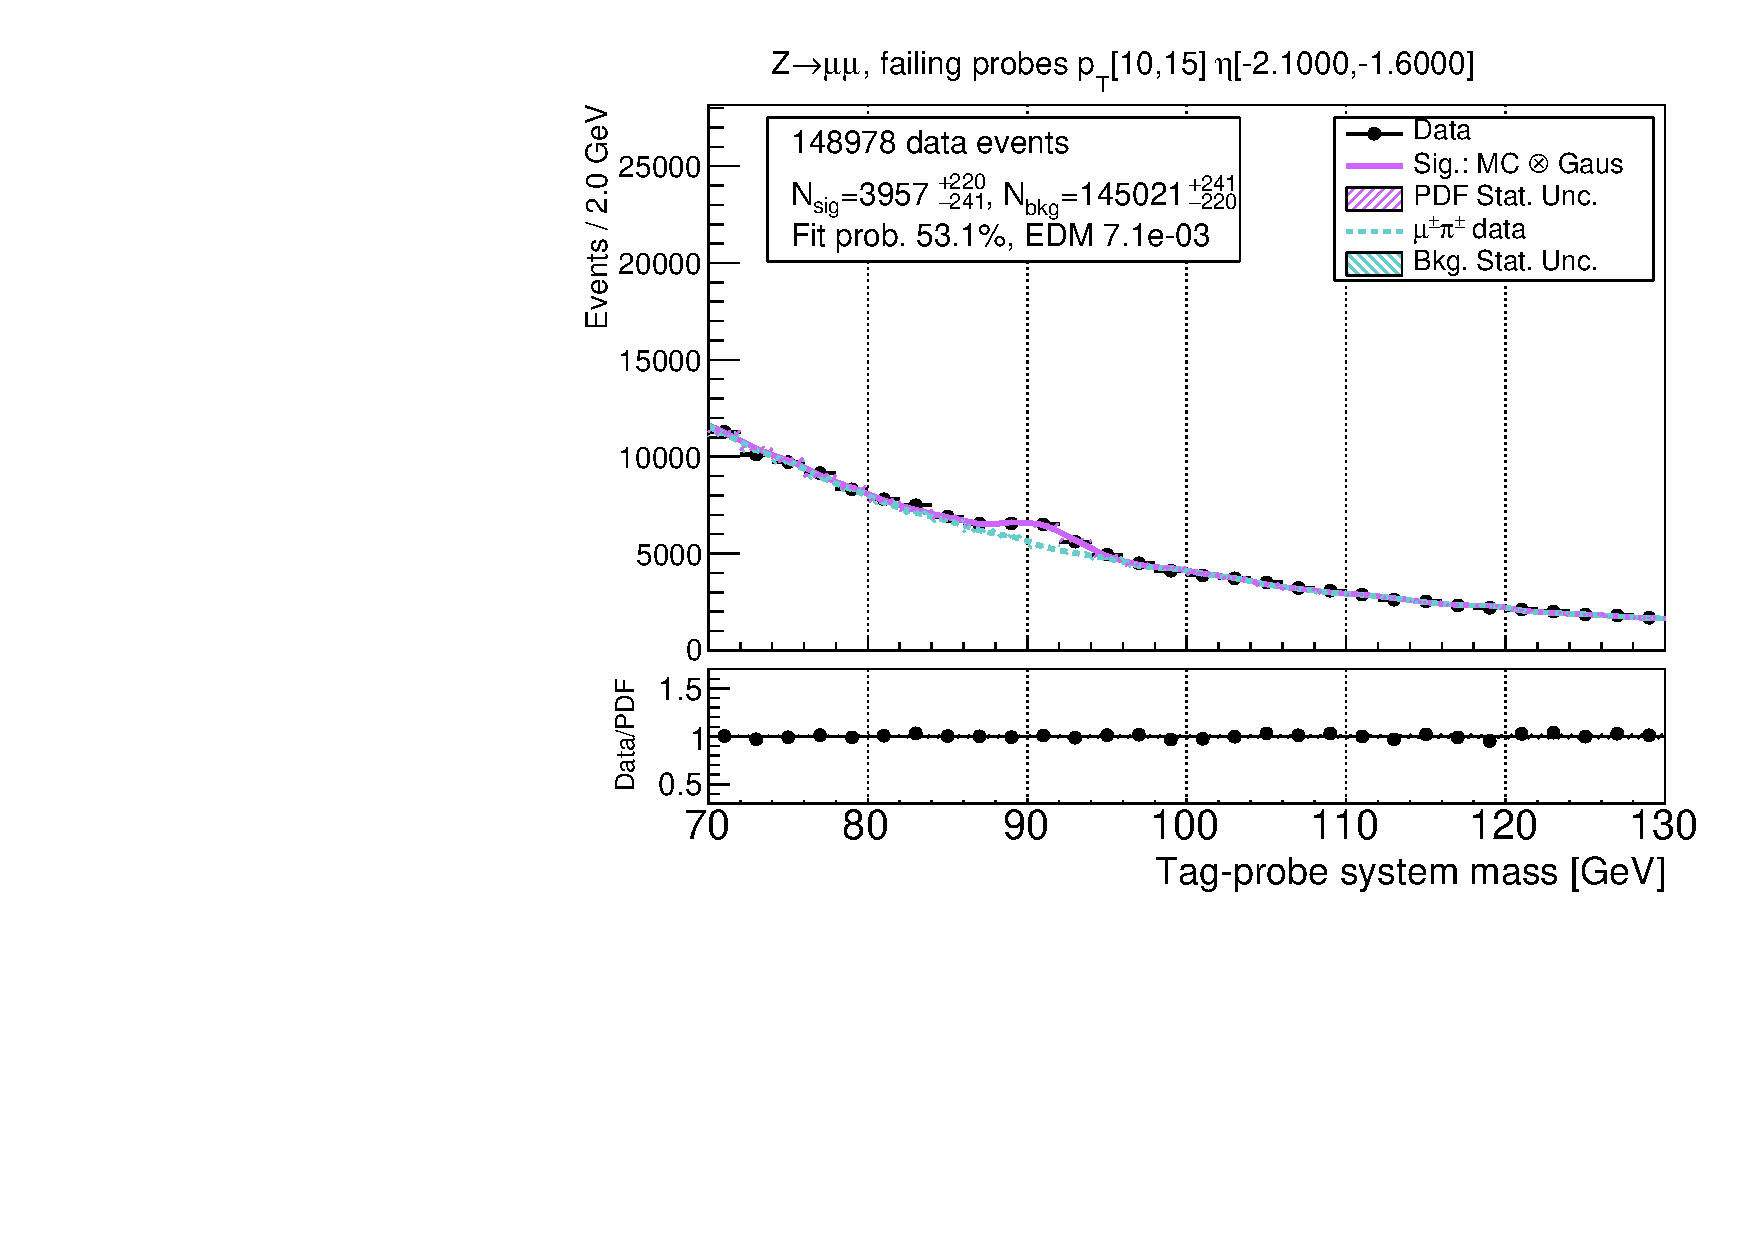
\includegraphics[width=0.49\textwidth]{figures/Zmm_RecoTemplate_BkgLPi_fail_ptBin0_etaBin1.pdf}
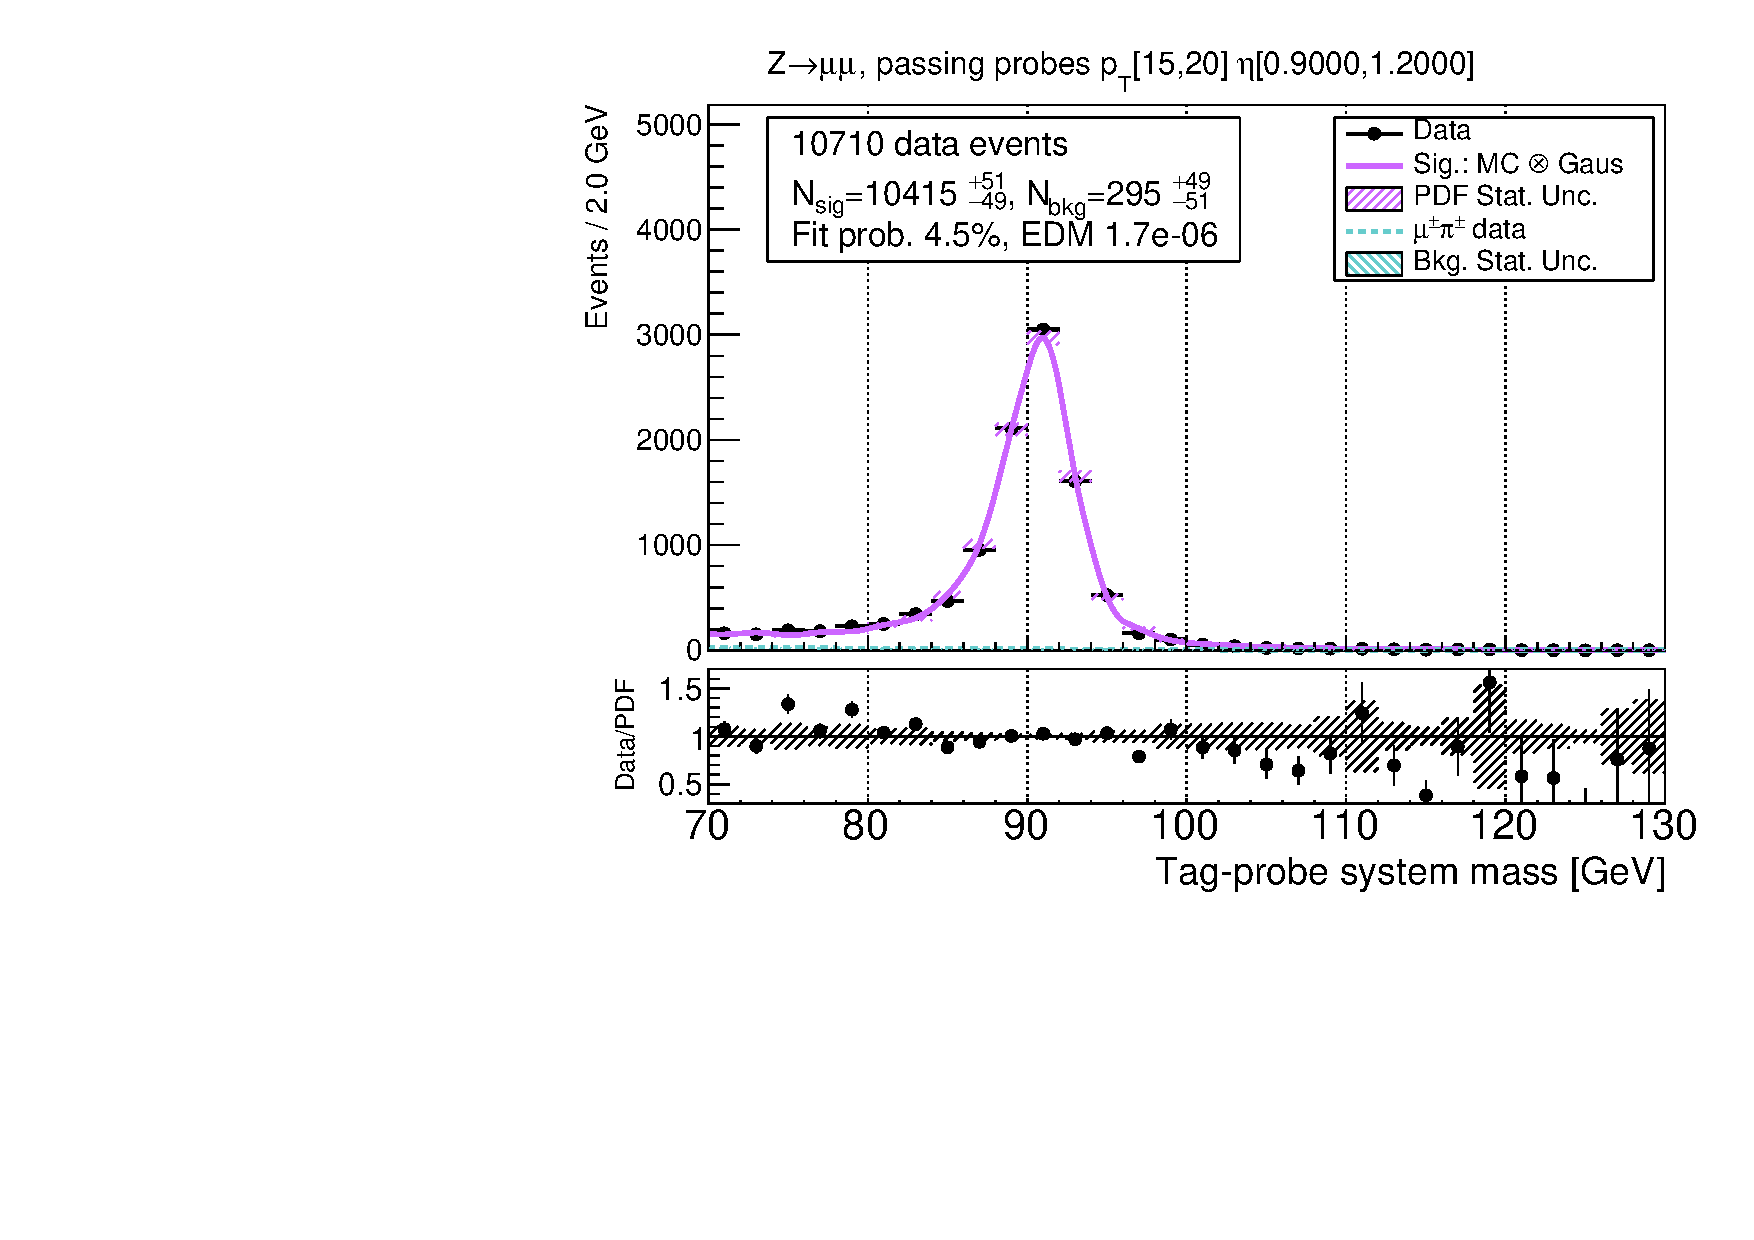
\includegraphics[width=0.49\textwidth]{figures/Zmm_RecoTemplate_BkgLPi_pass_ptBin1_etaBin9.pdf}
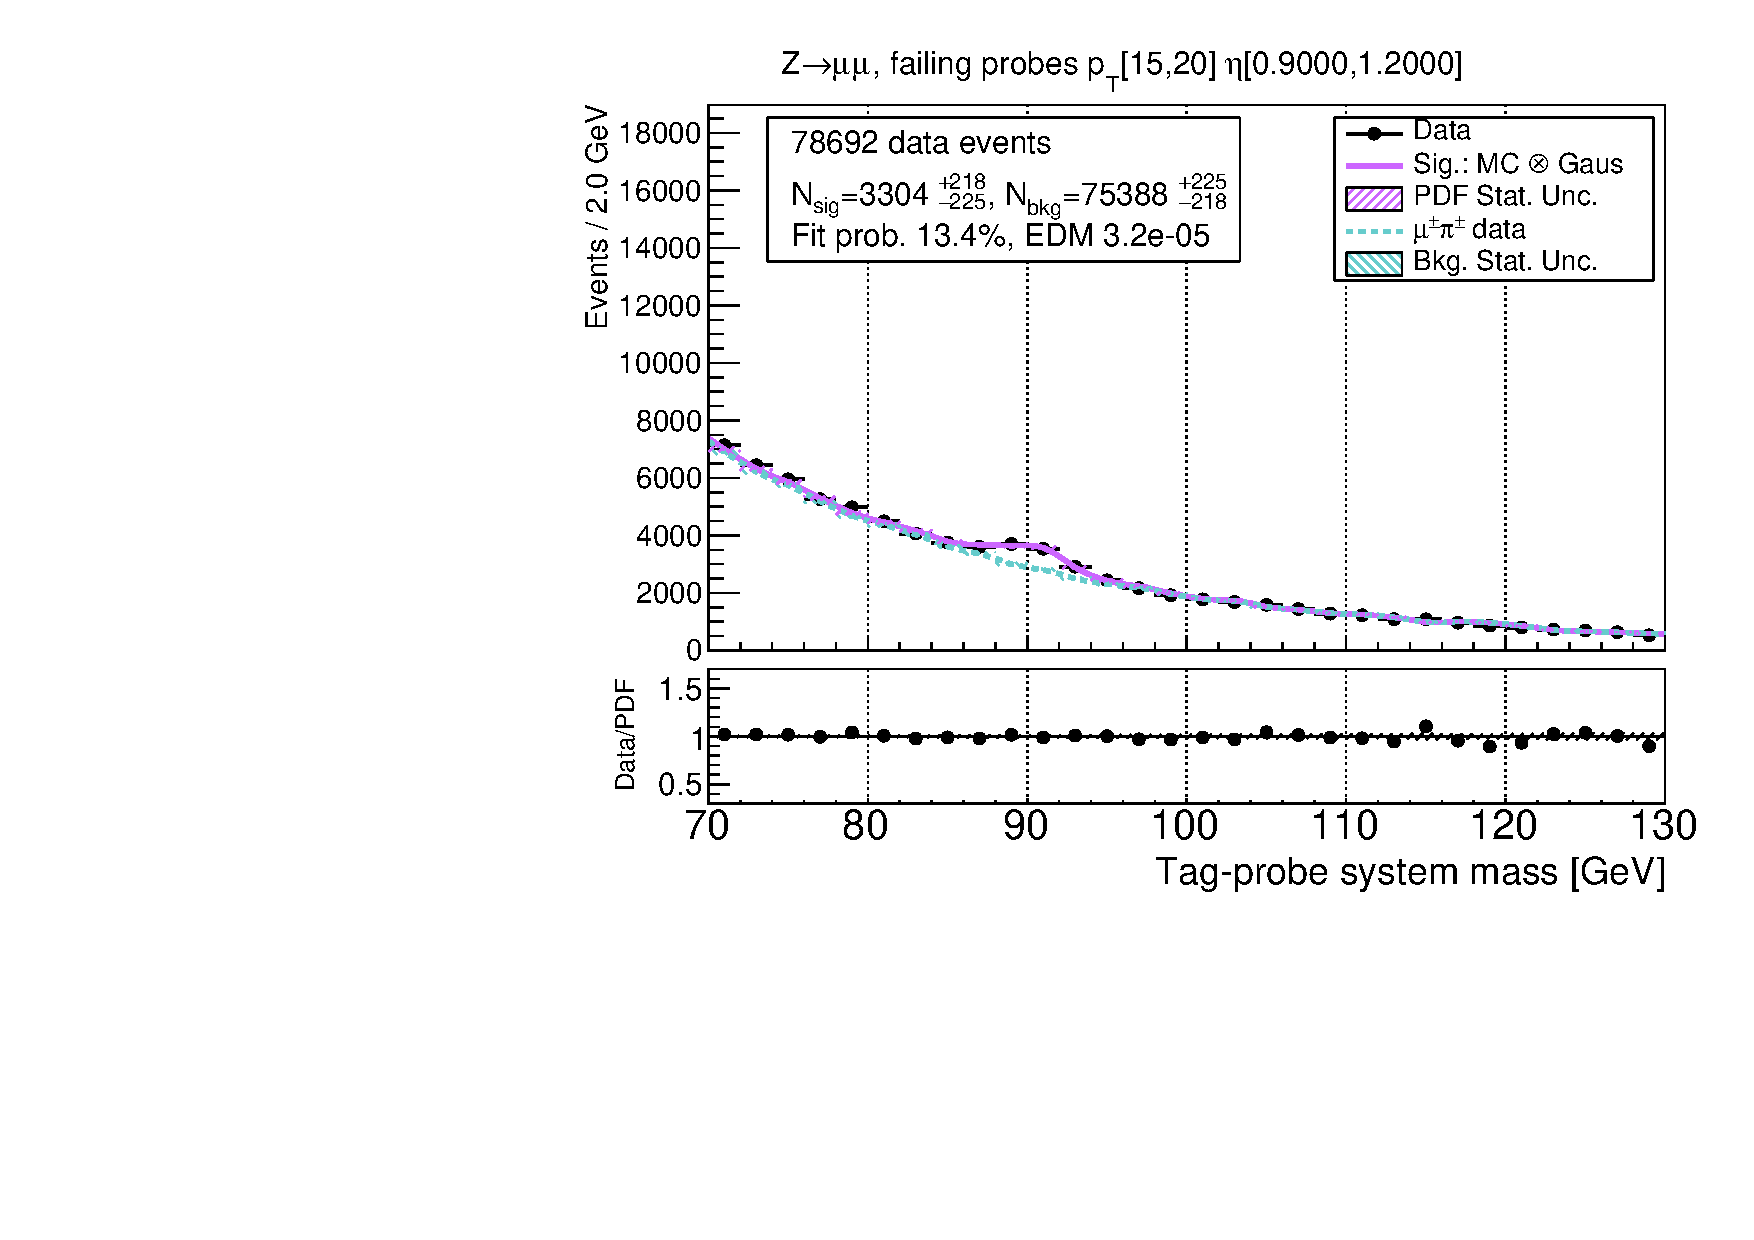
\includegraphics[width=0.49\textwidth]{figures/Zmm_RecoTemplate_BkgLPi_fail_ptBin1_etaBin9.pdf}
\caption{Efficiency extraction fits for the Medium muon working point using the data-driven background shape, at low muon transverse momentum.}
\label{fig:ZmmNominalFits1}
\end{figure}
\begin{figure}
\centering
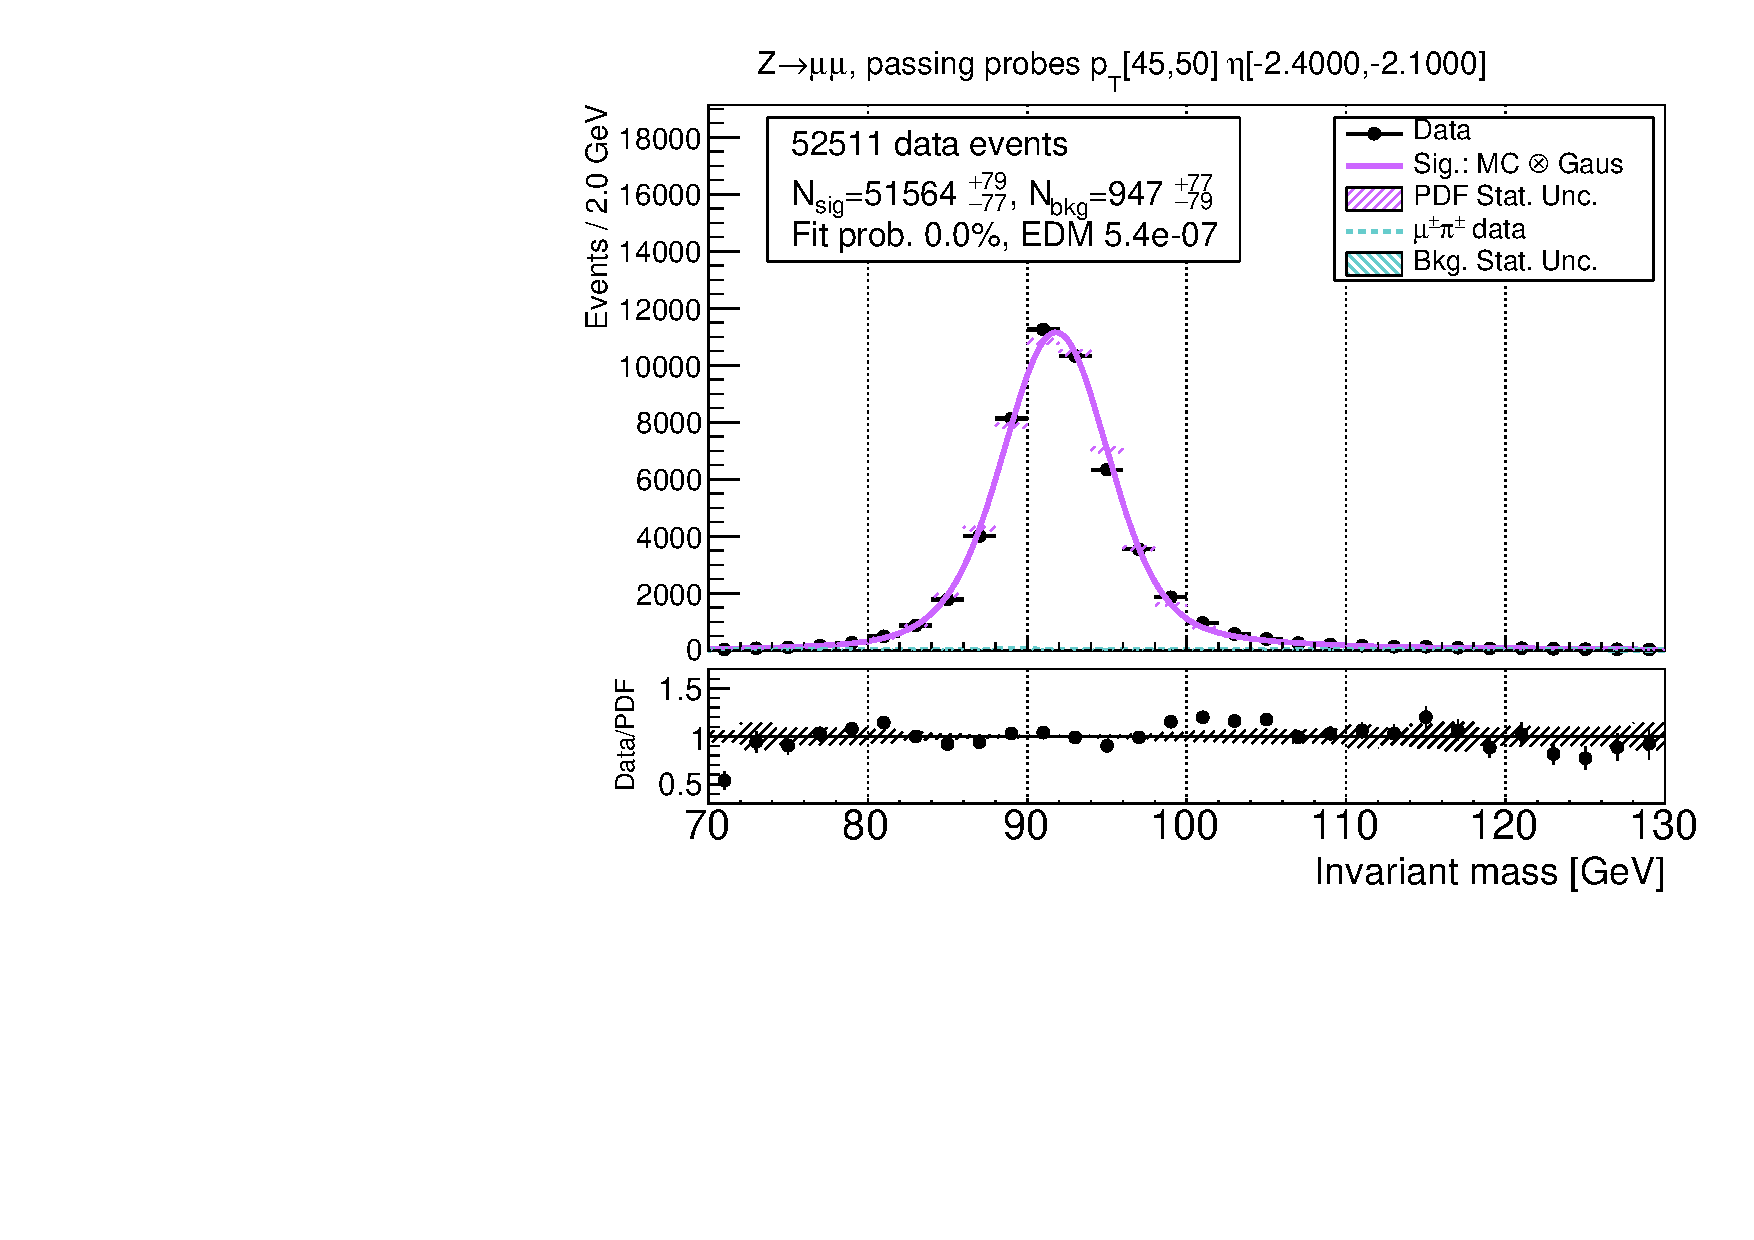
\includegraphics[width=0.49\textwidth]{figures/Zmm_RecoTemplate_BkgLPi_pass_ptBin7_etaBin0.pdf}
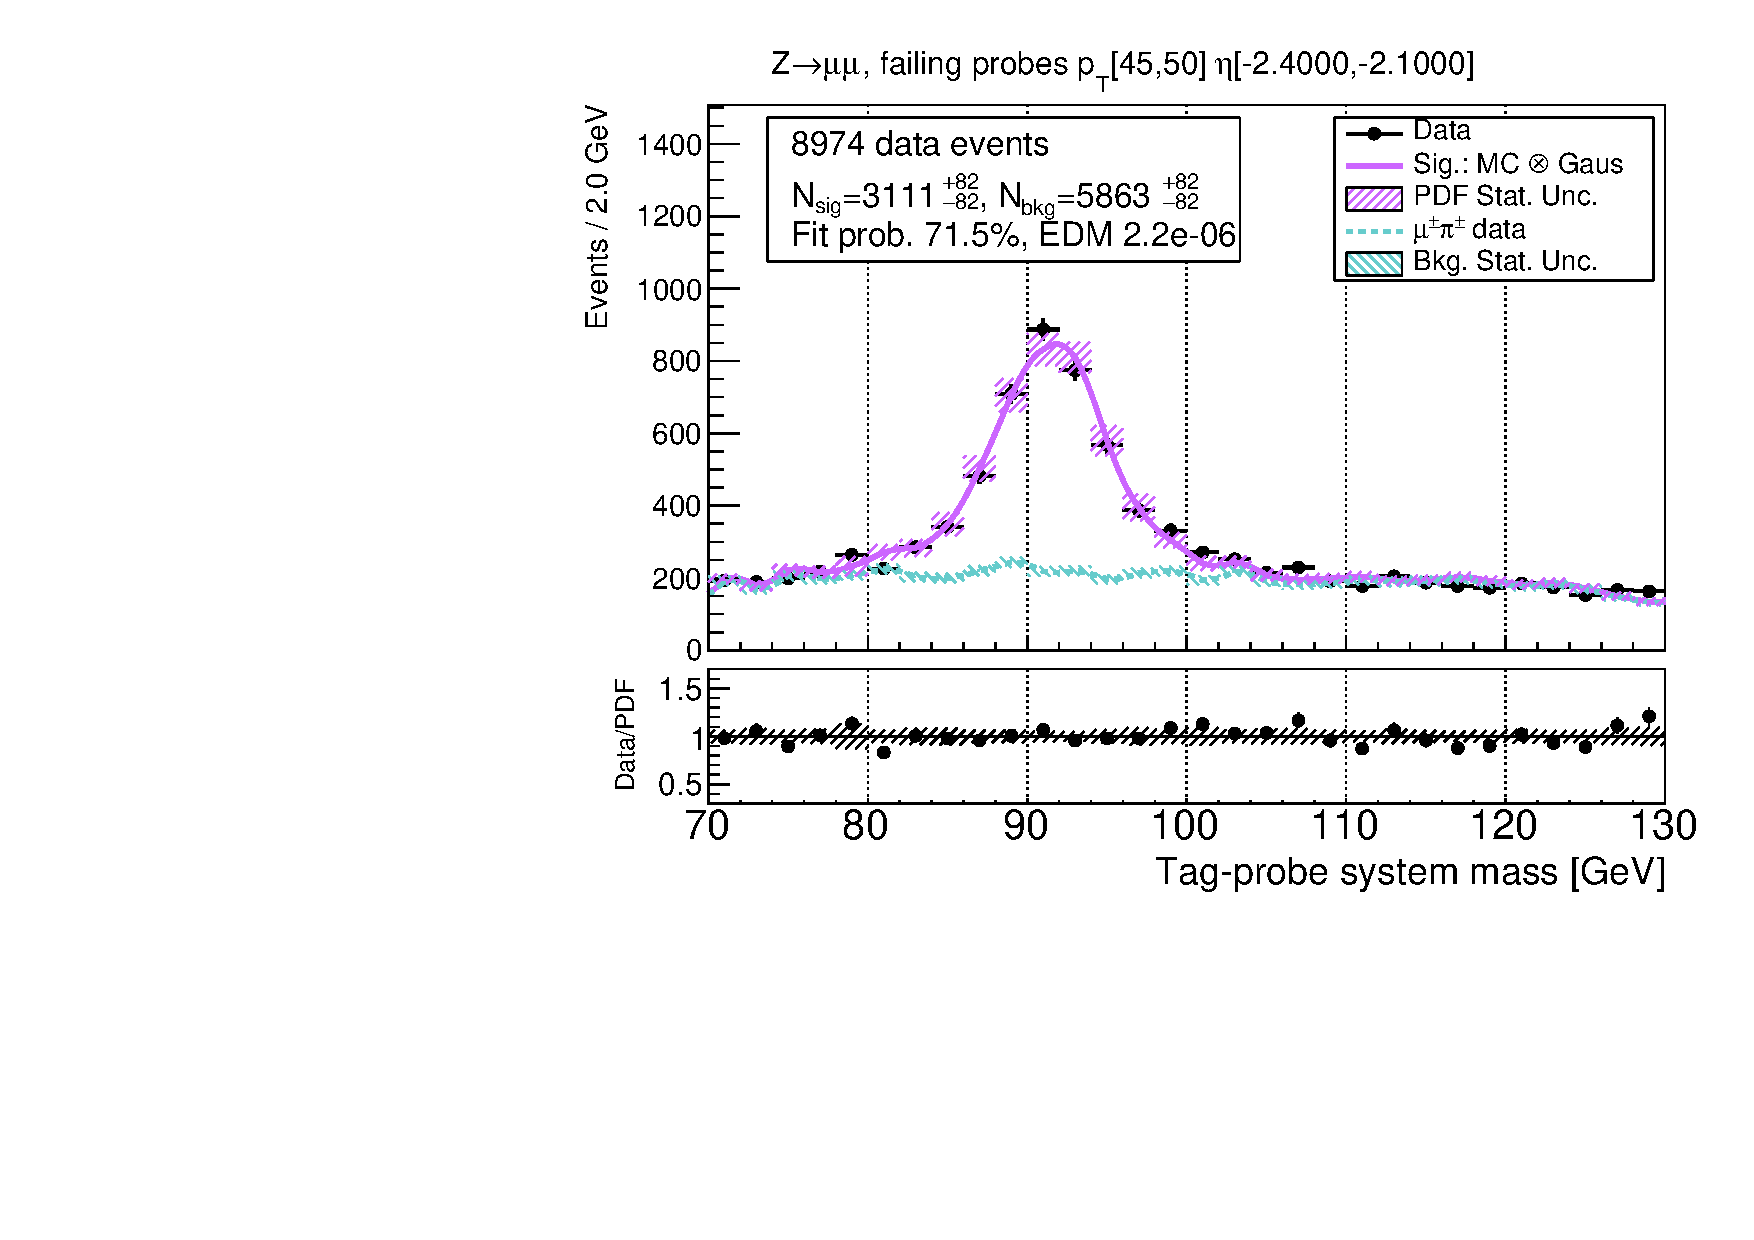
\includegraphics[width=0.49\textwidth]{figures/Zmm_RecoTemplate_BkgLPi_fail_ptBin7_etaBin0.pdf}
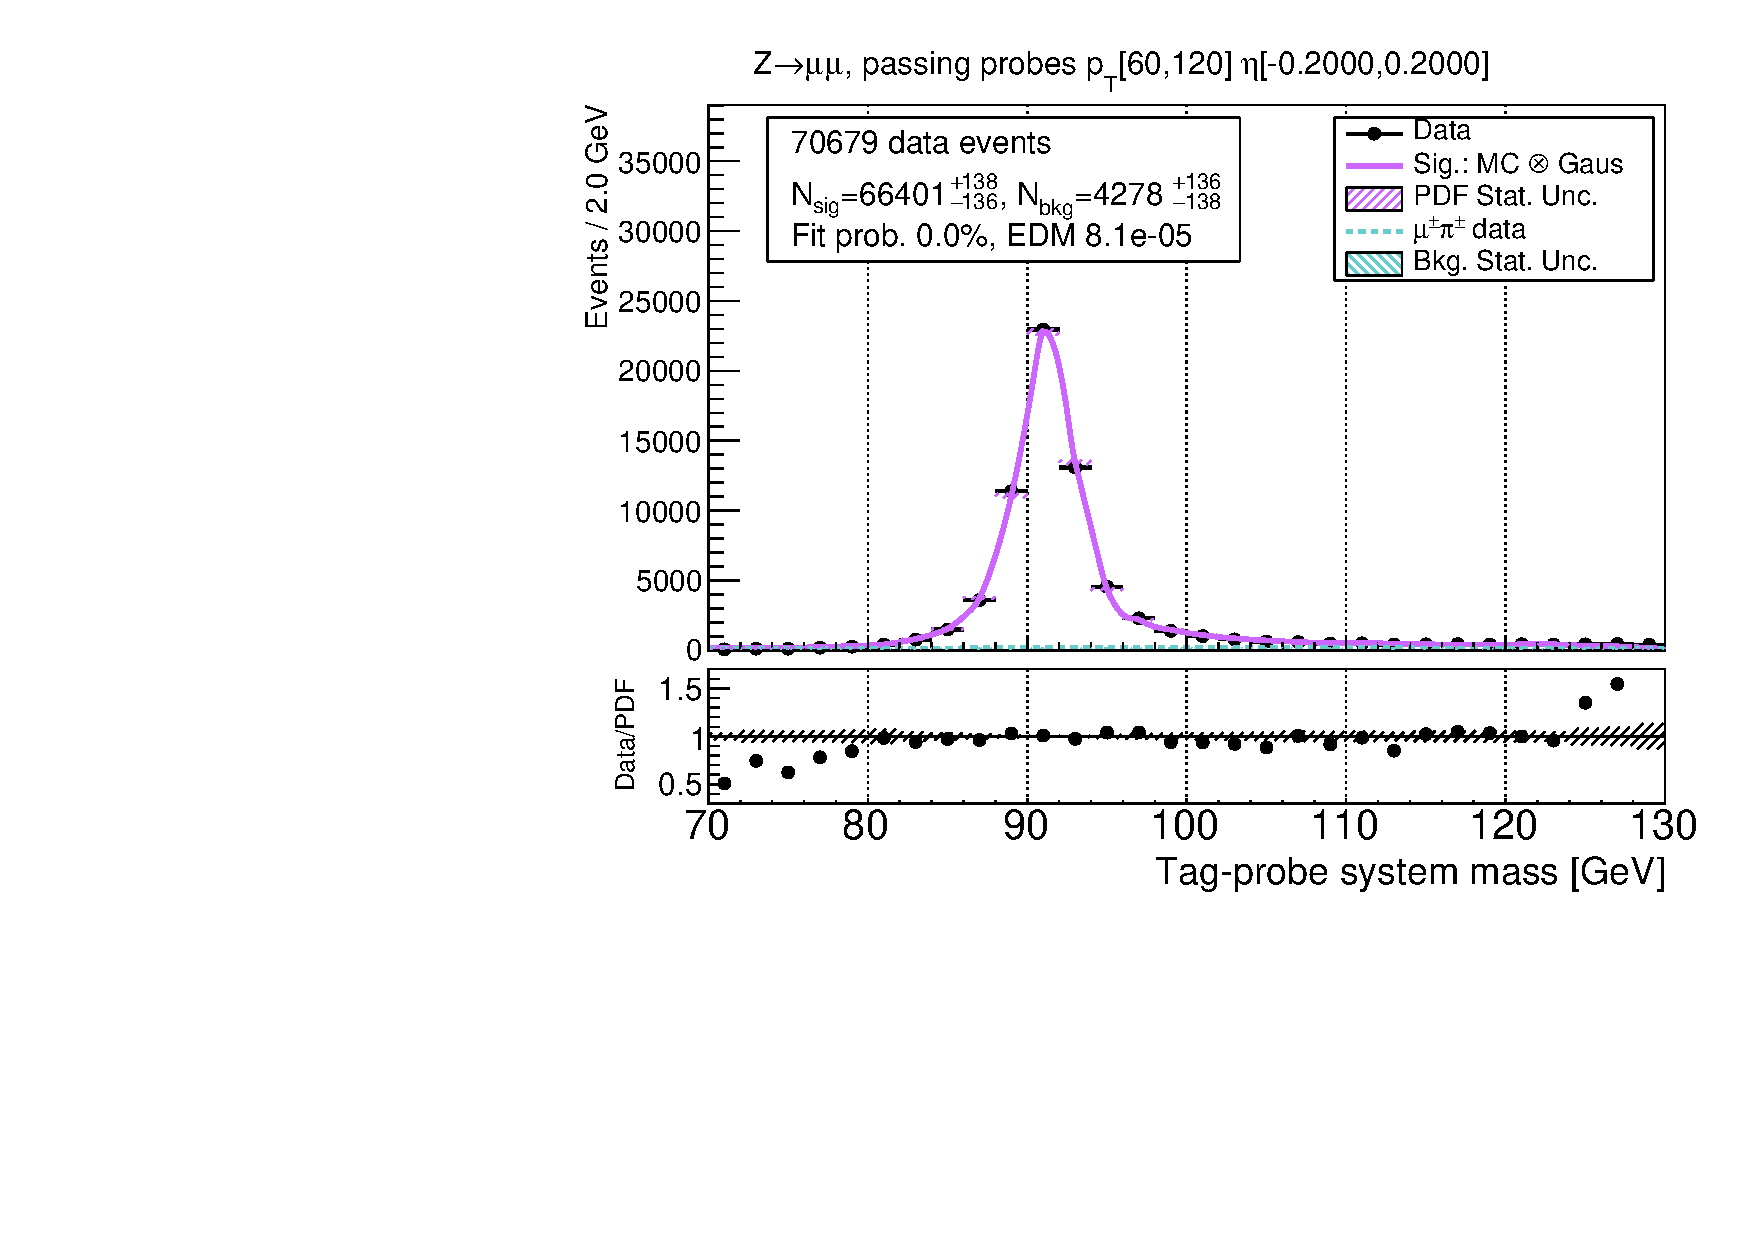
\includegraphics[width=0.49\textwidth]{figures/Zmm_RecoTemplate_BkgLPi_pass_ptBin10_etaBin6.pdf}
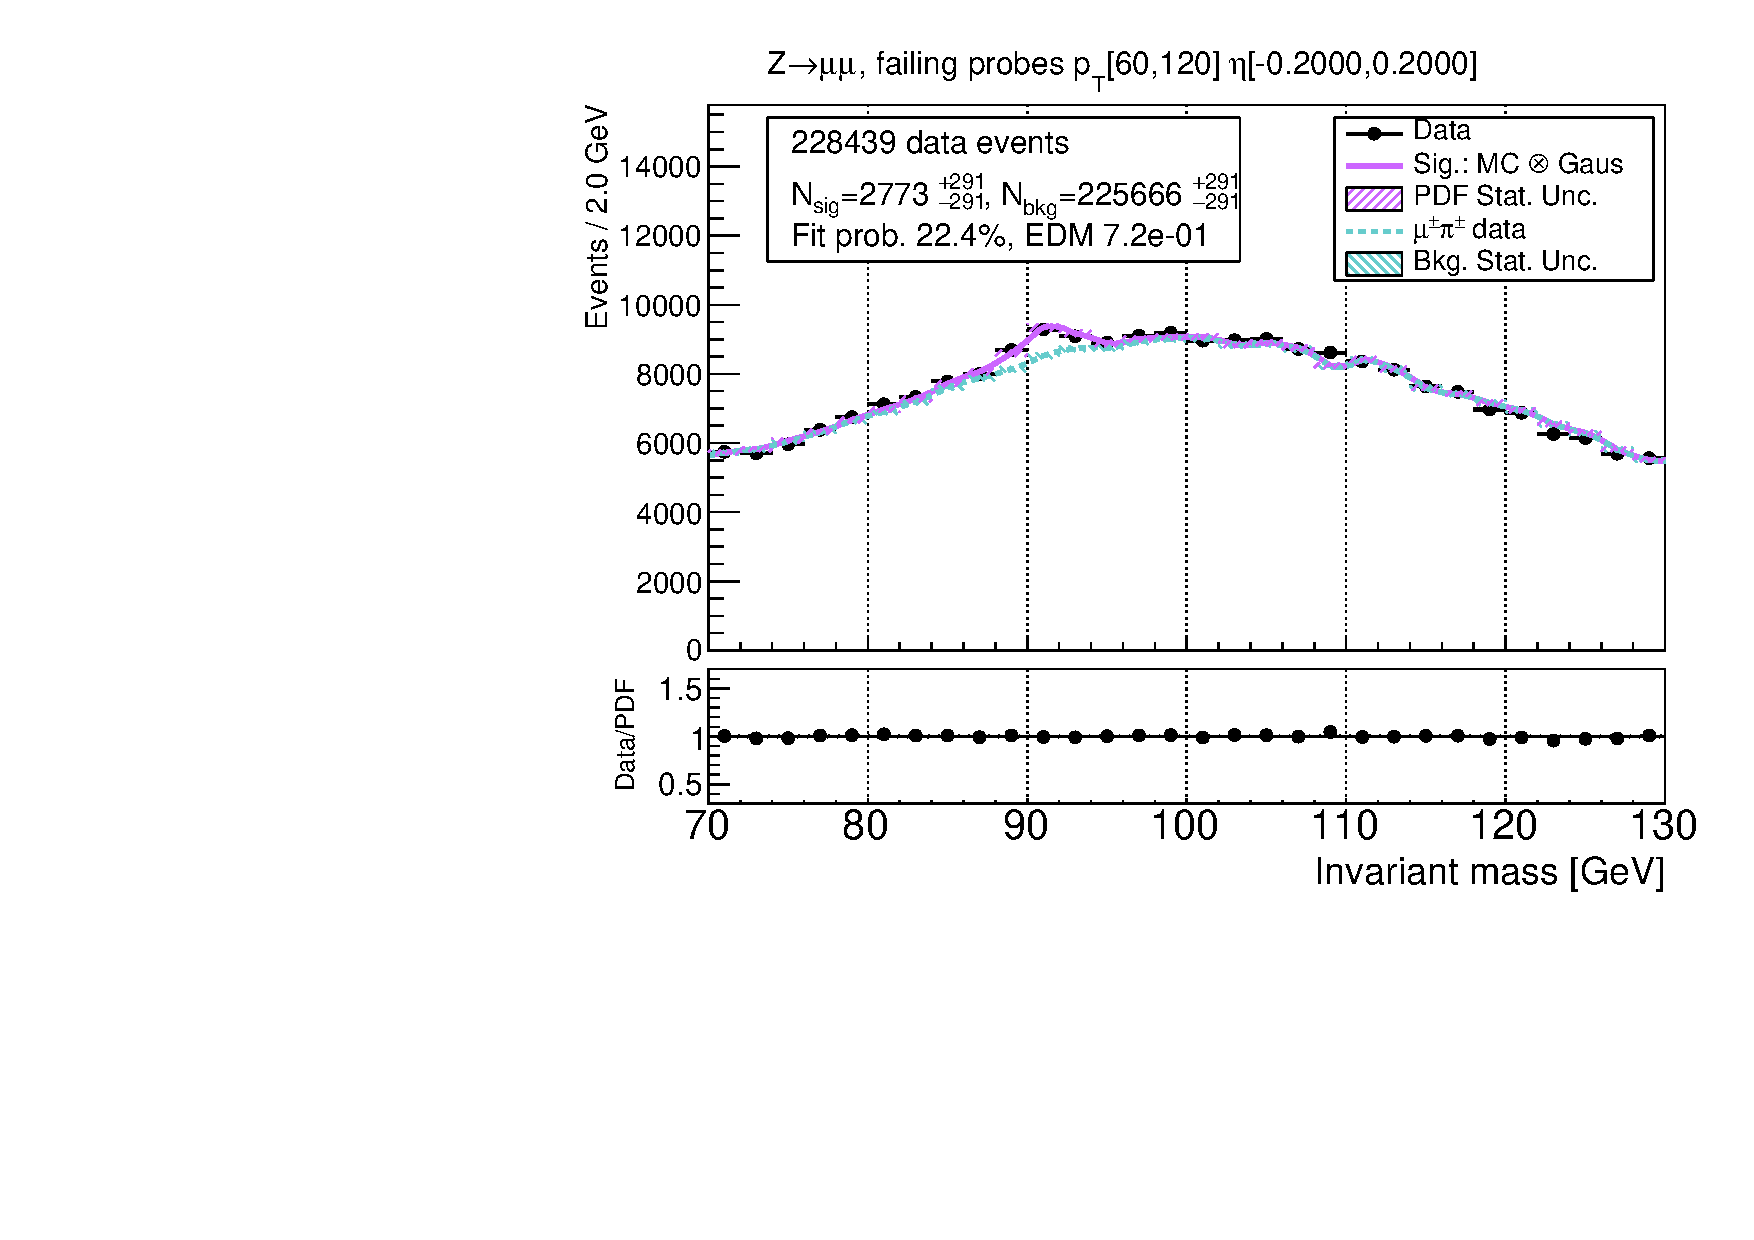
\includegraphics[width=0.49\textwidth]{figures/Zmm_RecoTemplate_BkgLPi_fail_ptBin10_etaBin6.pdf}
\caption{Efficiency extraction fits for the Medium muon working point using the data-driven background shape, at higher values of muon transverse momentum.}
\label{fig:ZmmNominalFits2}
\end{figure}

\begin{figure}
\centering
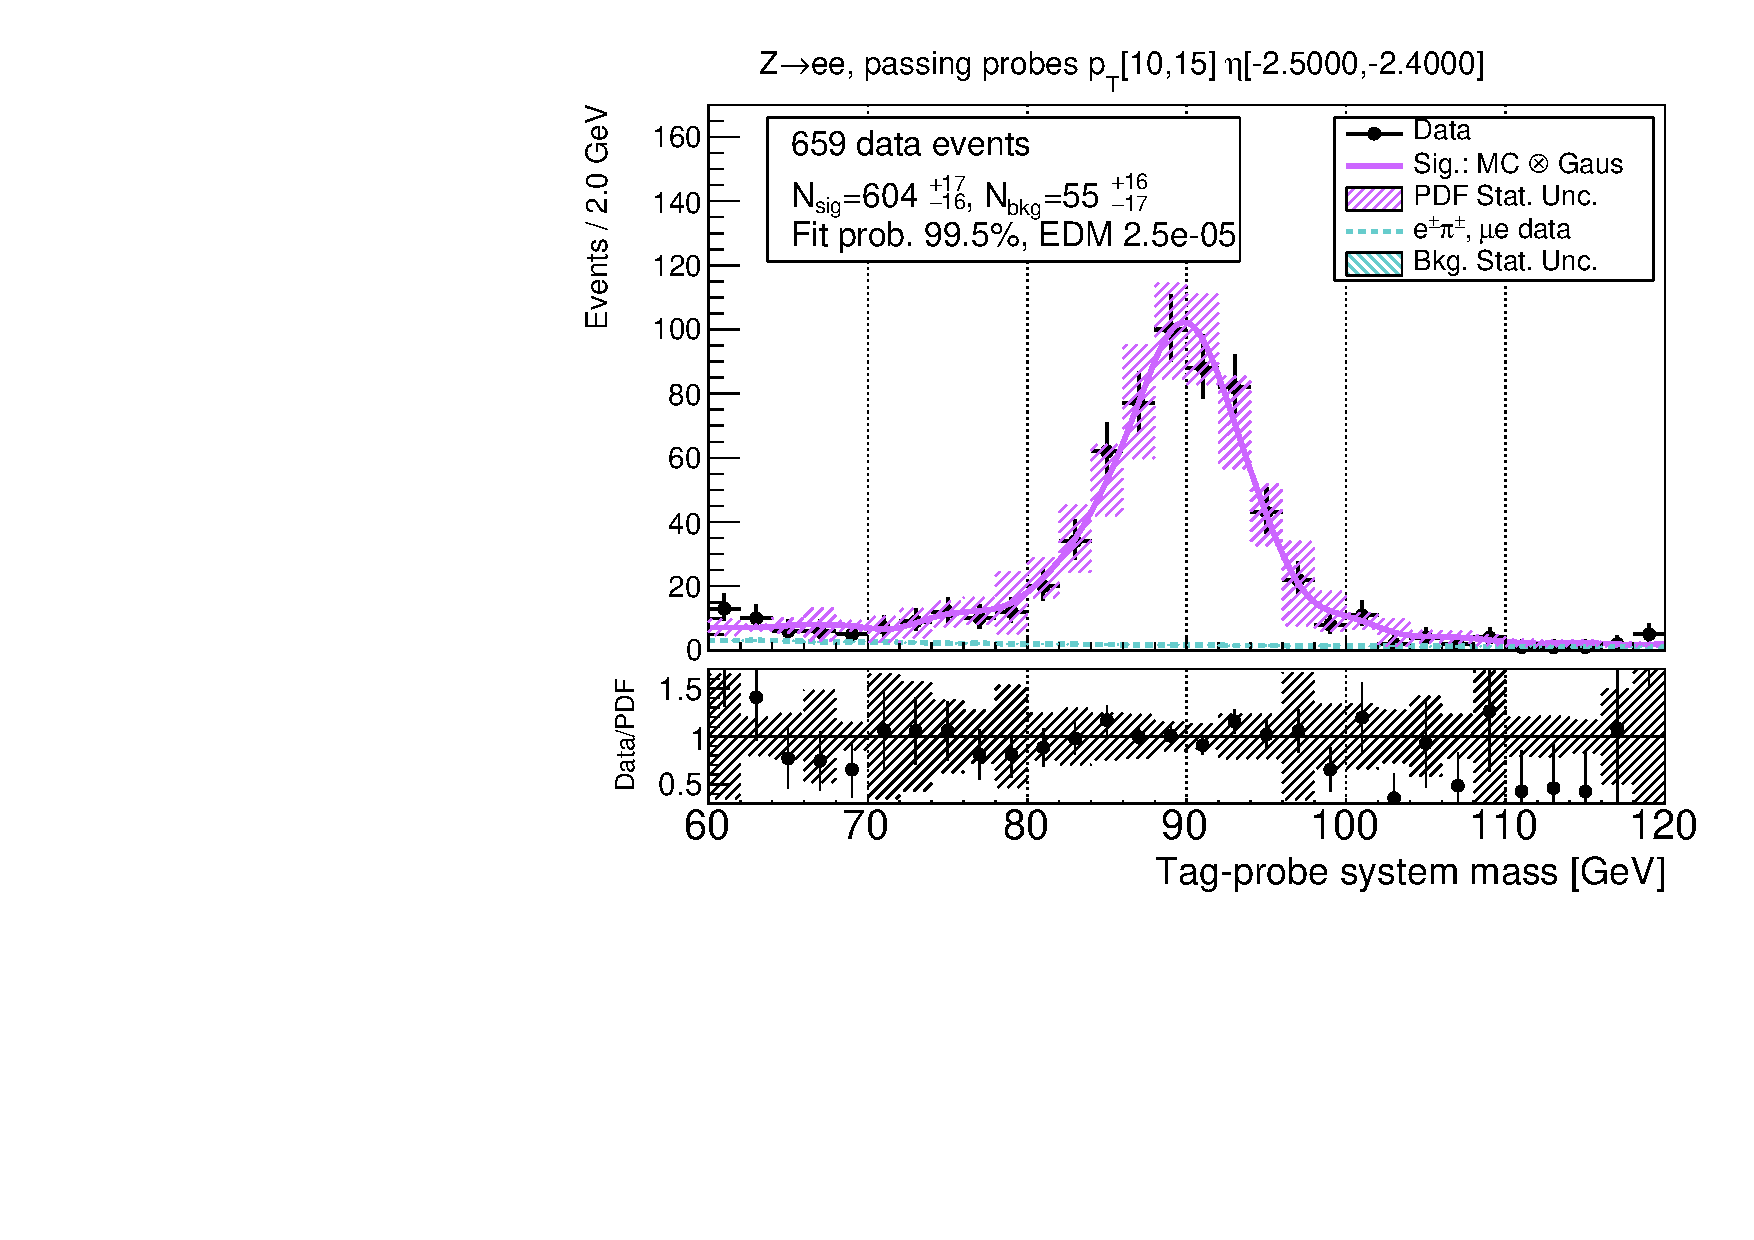
\includegraphics[width=0.49\textwidth]{figures/Zee_RecoTemplate_BkgLPiEMu_pass_ptBin0_etaBin0.pdf}
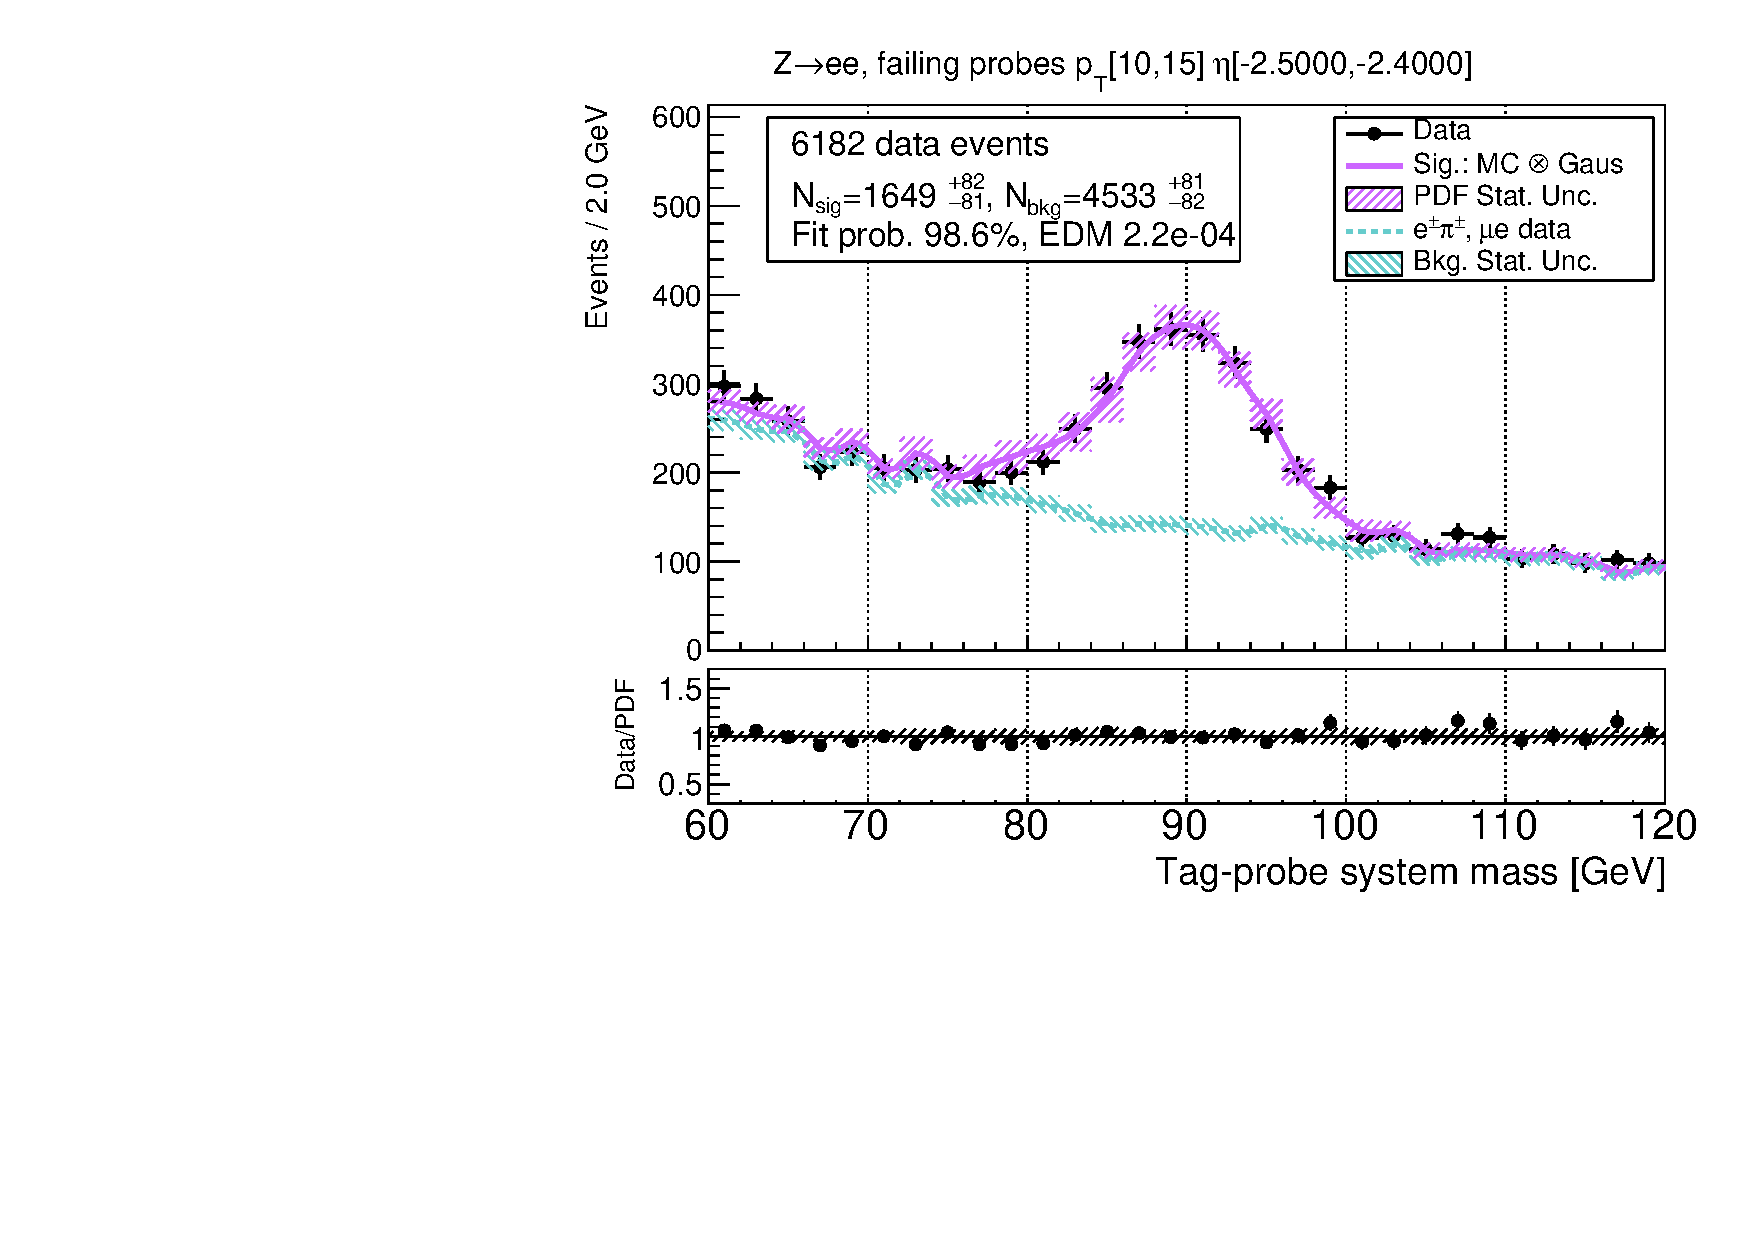
\includegraphics[width=0.49\textwidth]{figures/Zee_RecoTemplate_BkgLPiEMu_fail_ptBin0_etaBin0.pdf}
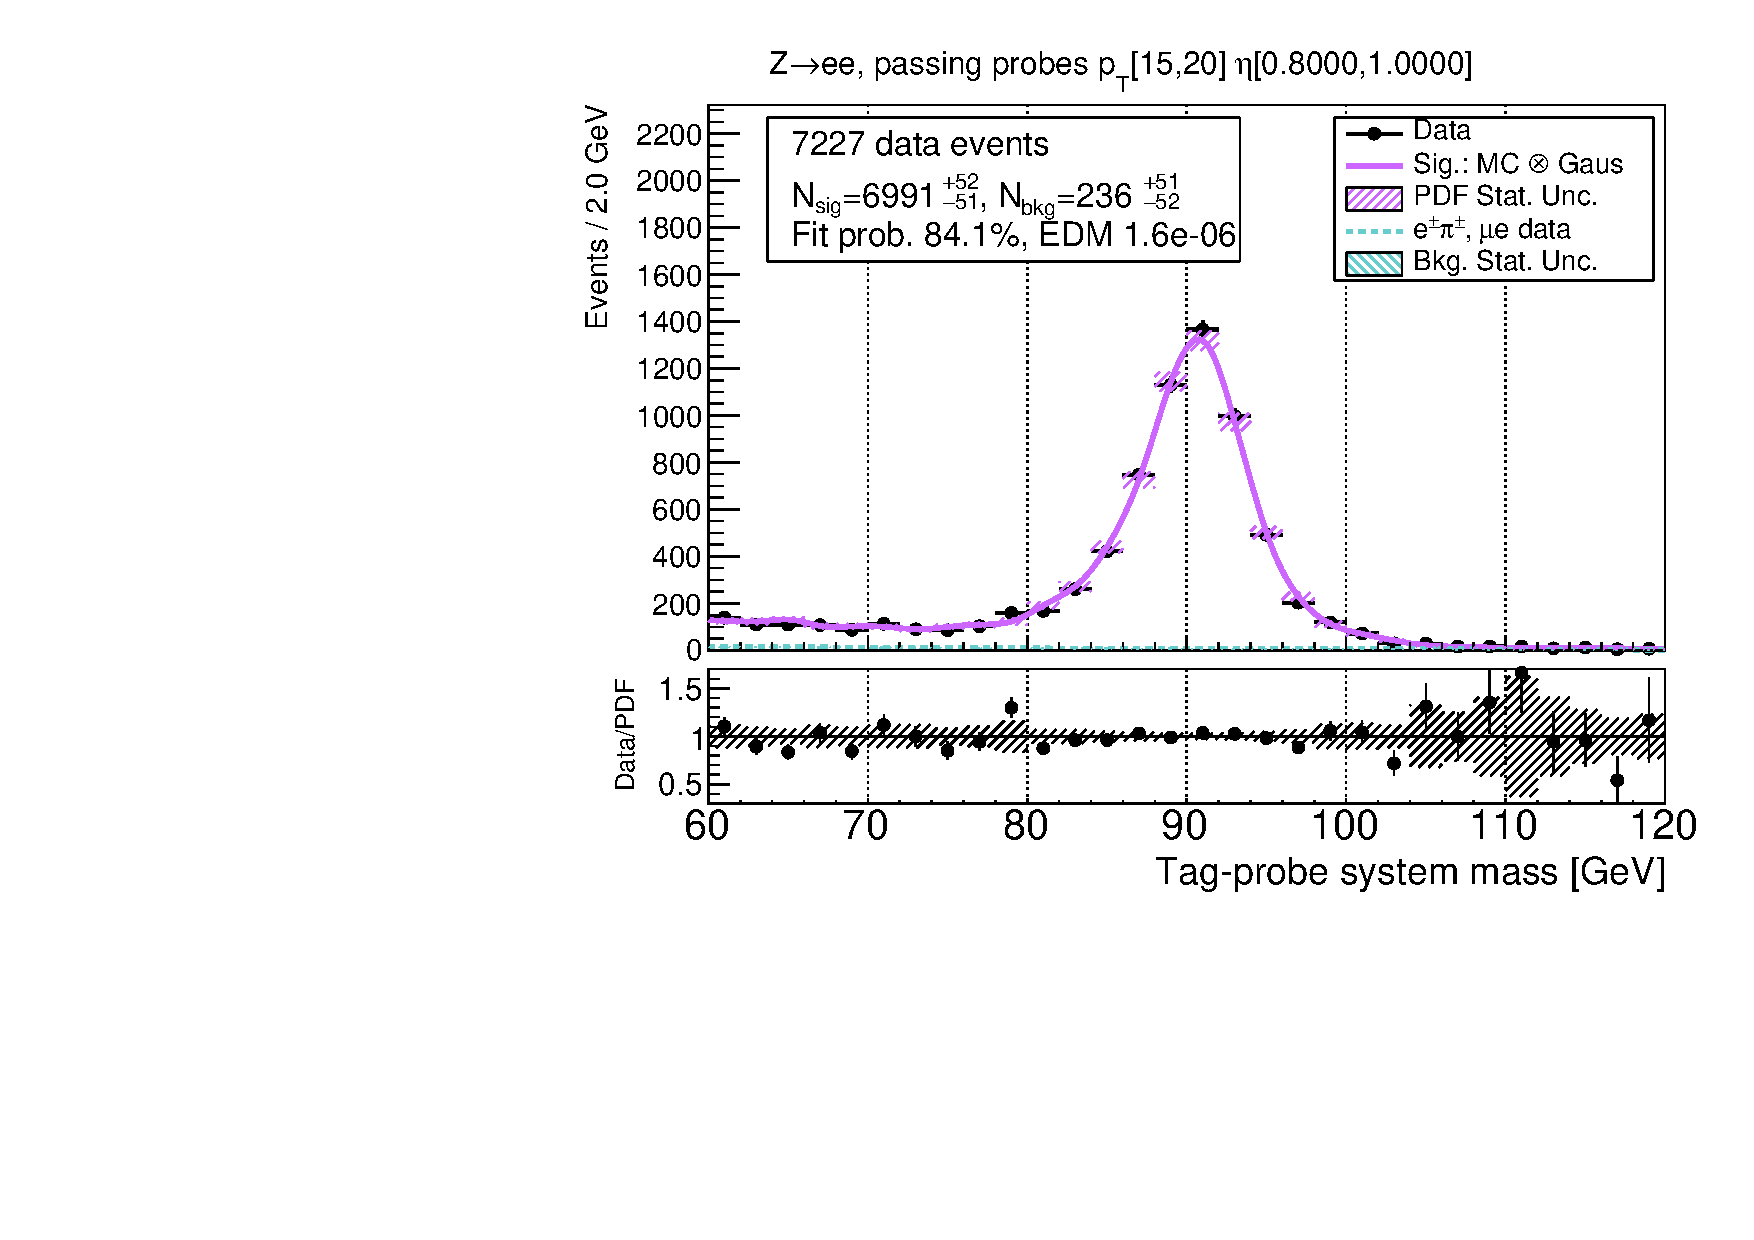
\includegraphics[width=0.49\textwidth]{figures/Zee_RecoTemplate_BkgLPiEMu_pass_ptBin1_etaBin19.pdf}
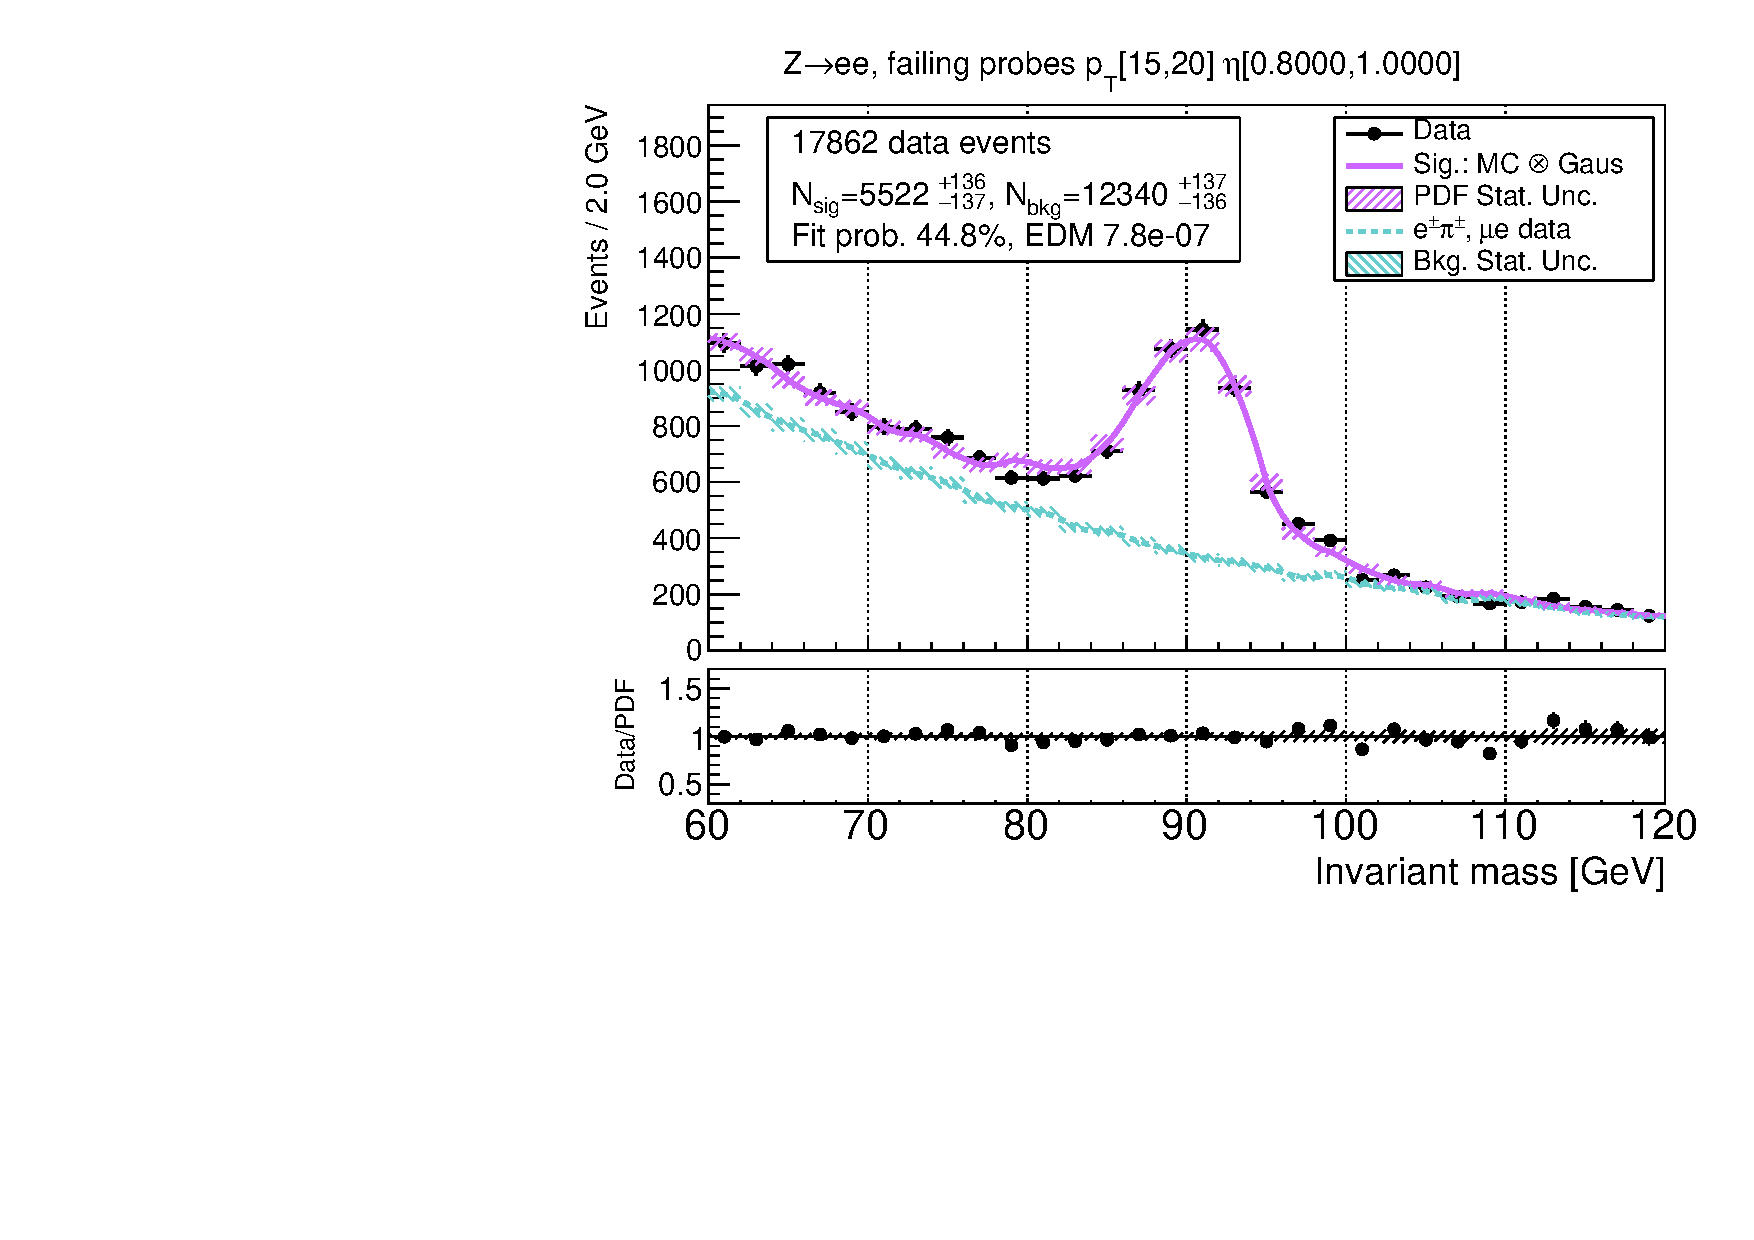
\includegraphics[width=0.49\textwidth]{figures/Zee_RecoTemplate_BkgLPiEMu_fail_ptBin1_etaBin19.pdf}
\caption{Efficiency extraction fits for the Medium electron working point using the data-driven background shape, at low electron transverse momentum.}
\label{fig:ZeeNominalFits1}
\end{figure}
\begin{figure}
\centering
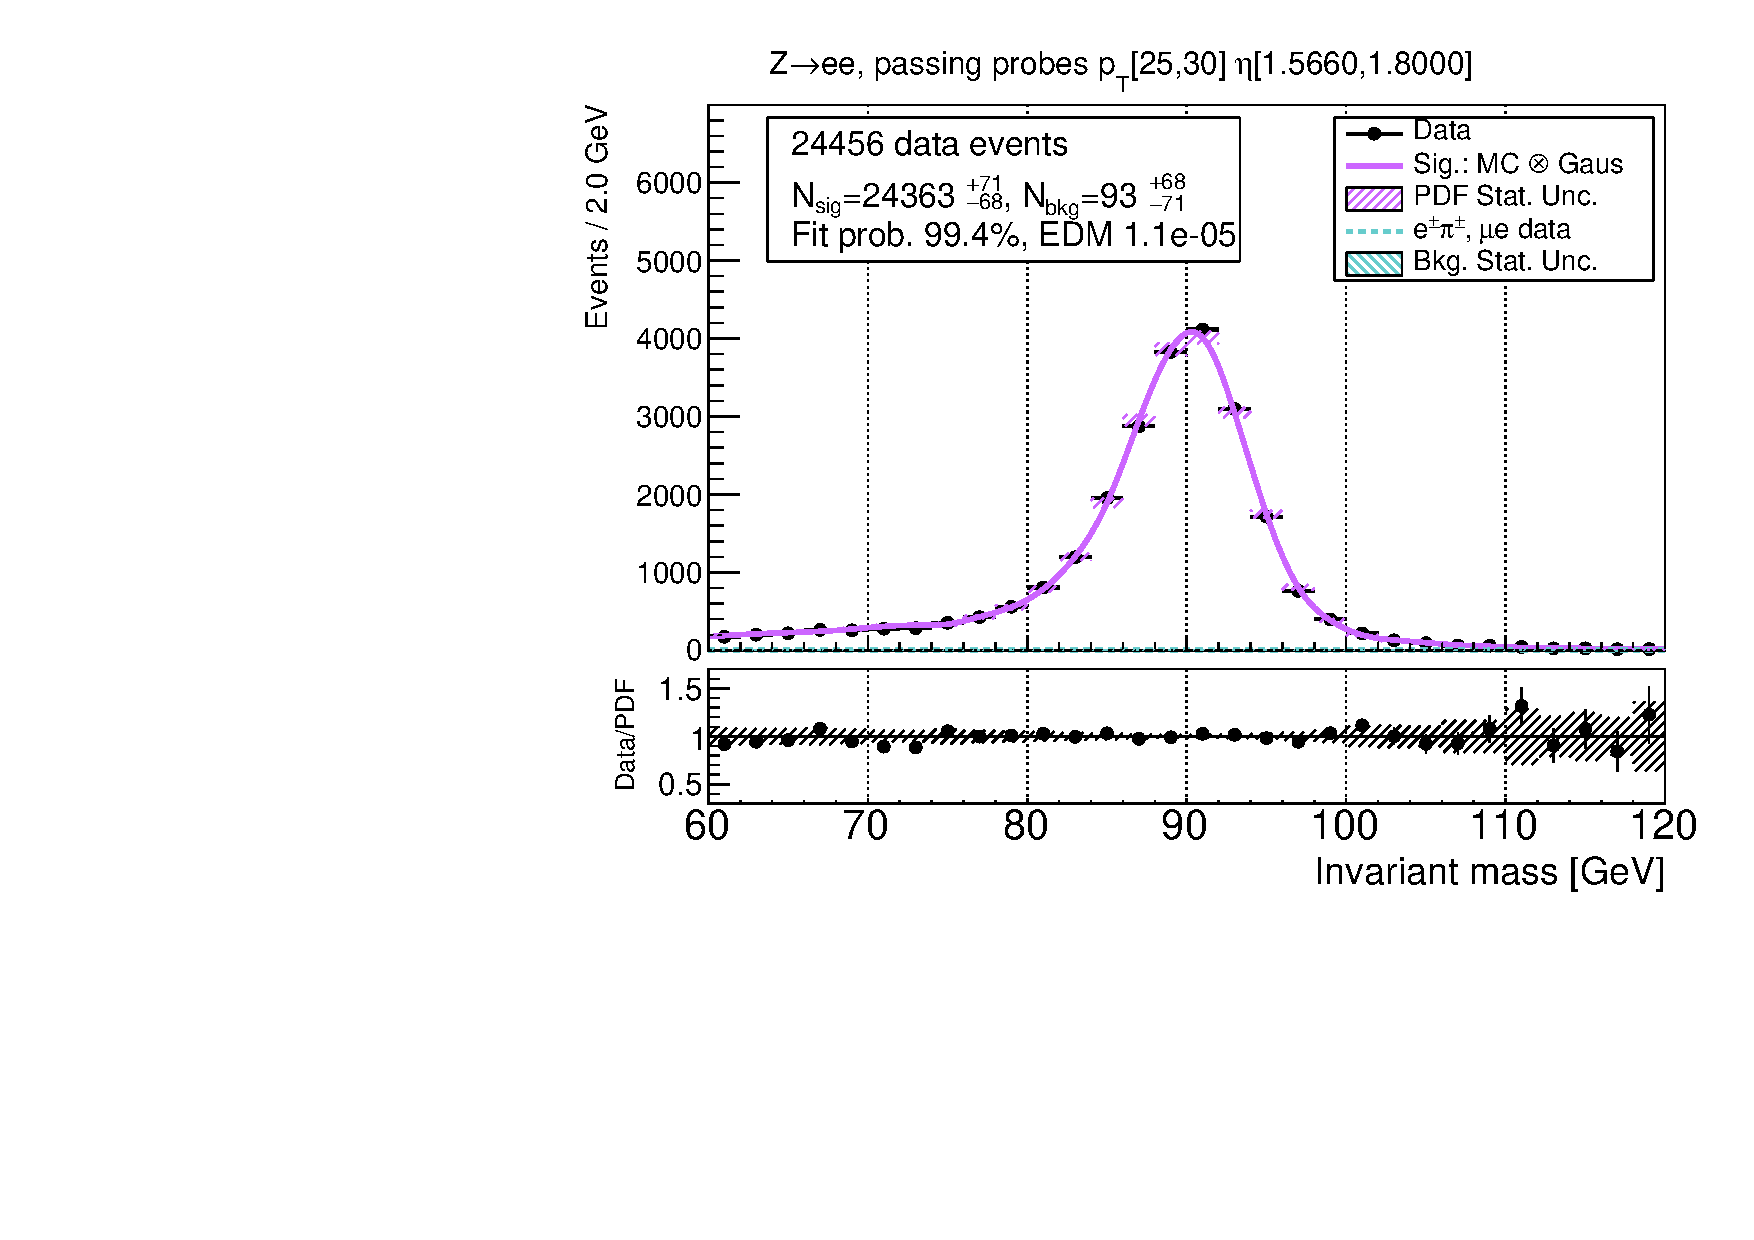
\includegraphics[width=0.49\textwidth]{figures/Zee_RecoTemplate_BkgLPiEMu_pass_ptBin3_etaBin23.pdf}
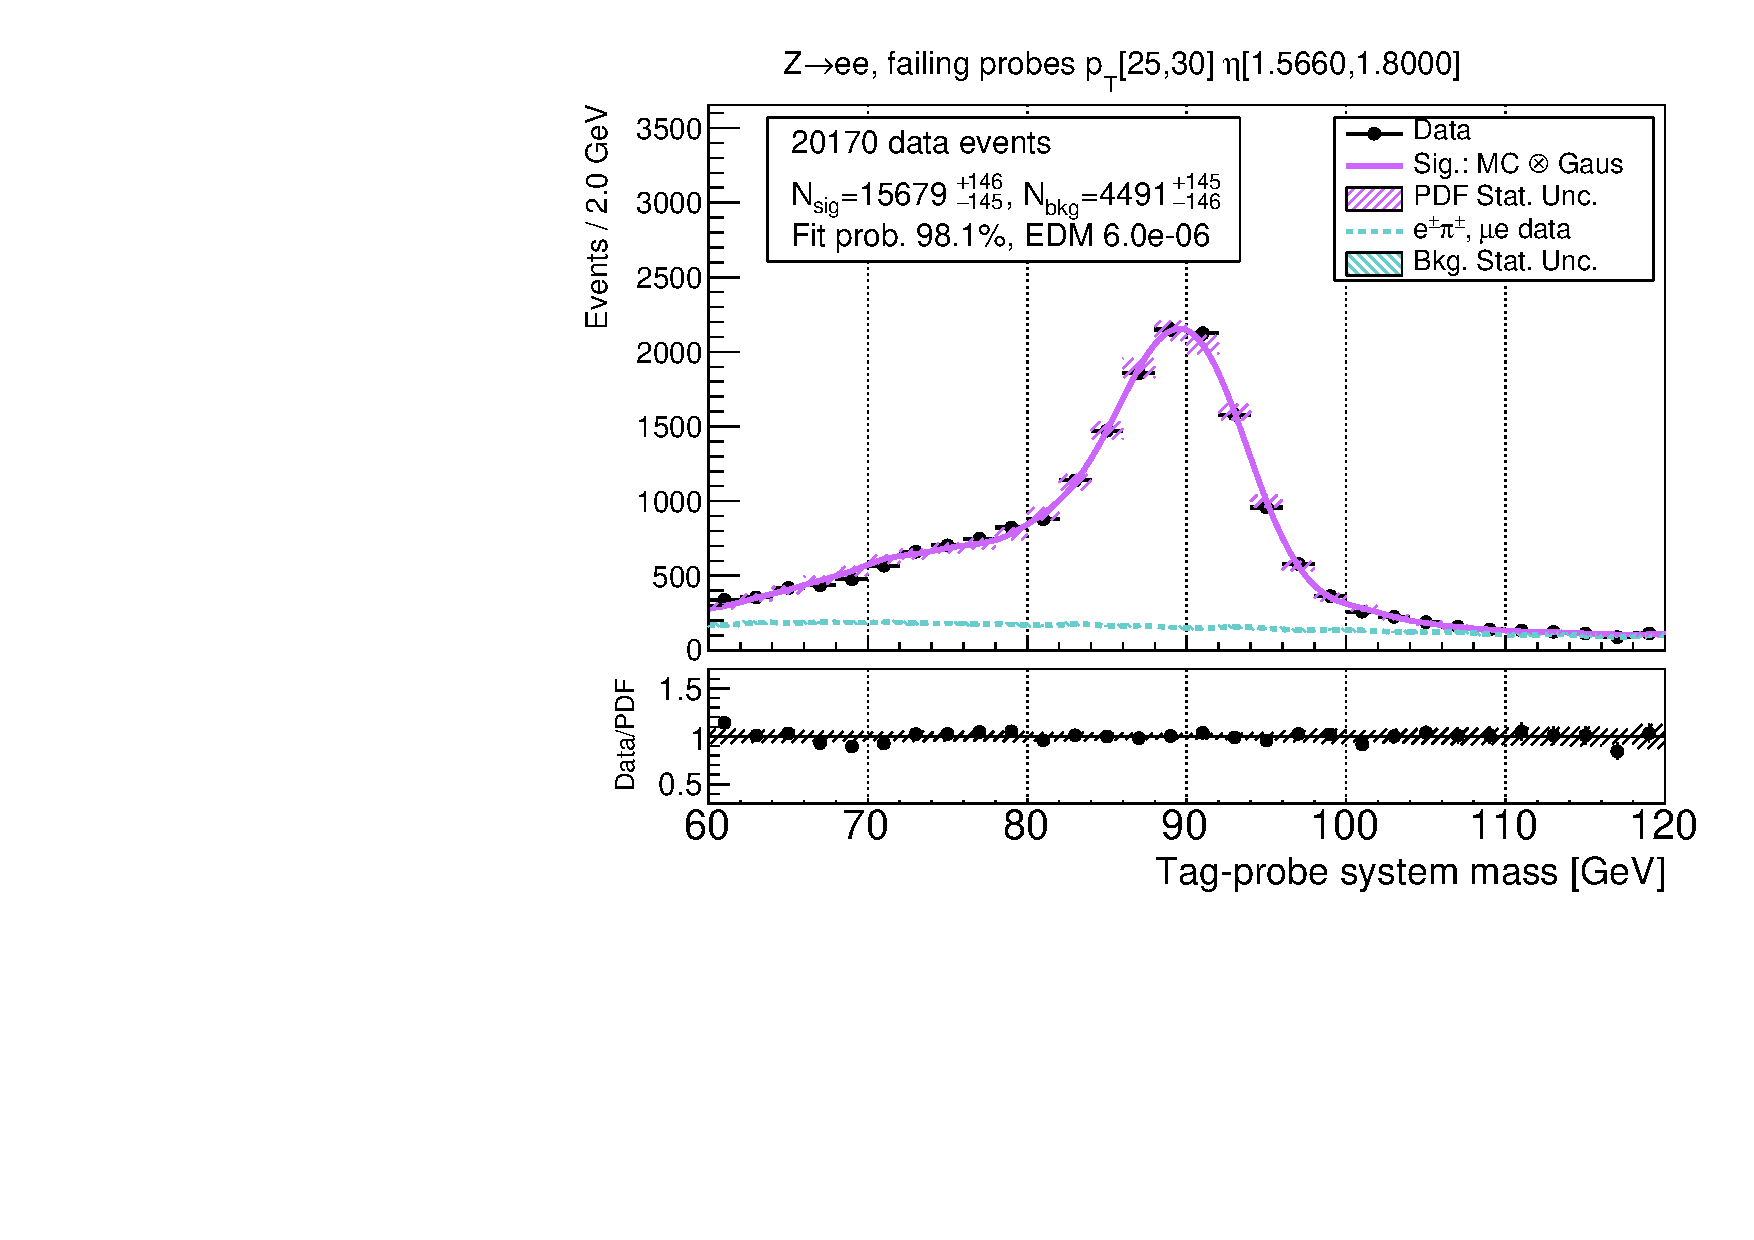
\includegraphics[width=0.49\textwidth]{figures/Zee_RecoTemplate_BkgLPiEMu_fail_ptBin3_etaBin23.pdf}
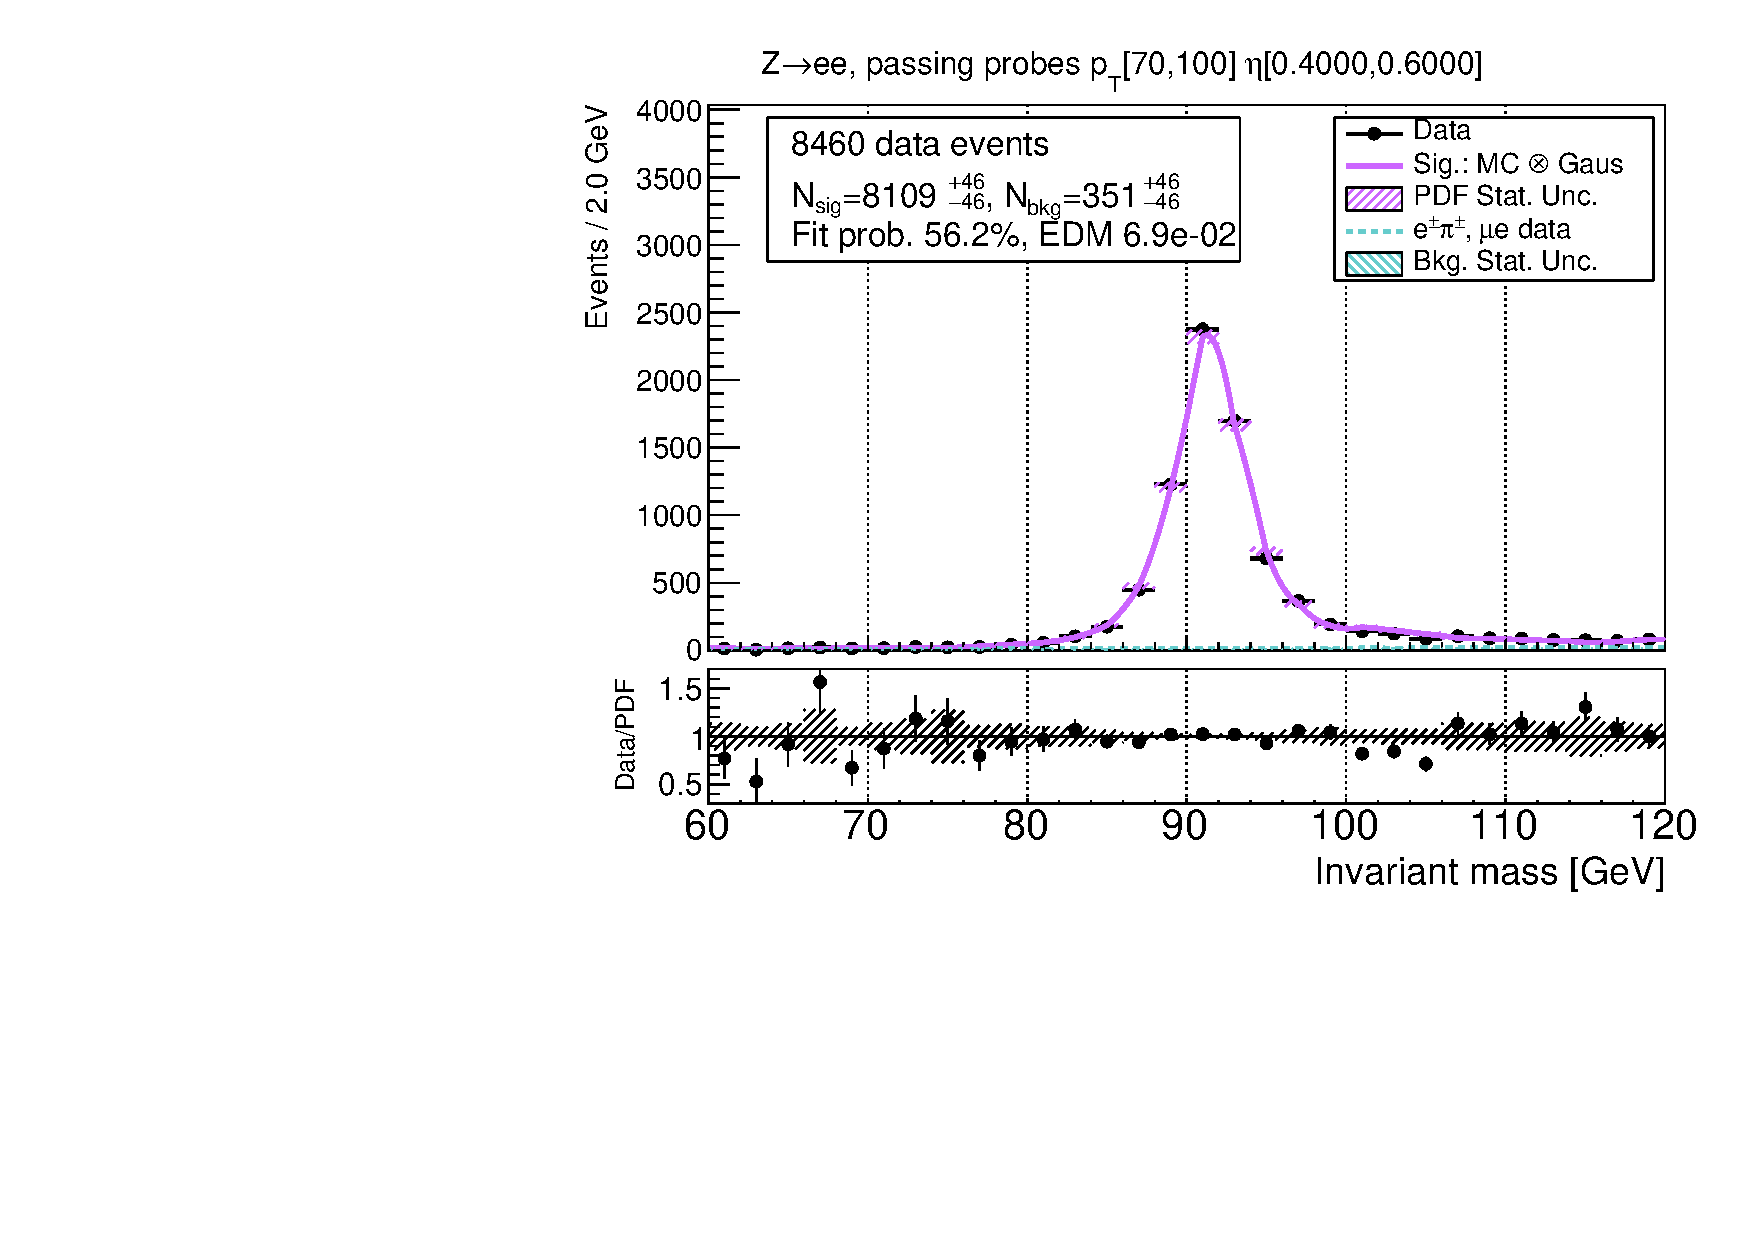
\includegraphics[width=0.49\textwidth]{figures/Zee_RecoTemplate_BkgLPiEMu_pass_ptBin14_etaBin17.pdf}
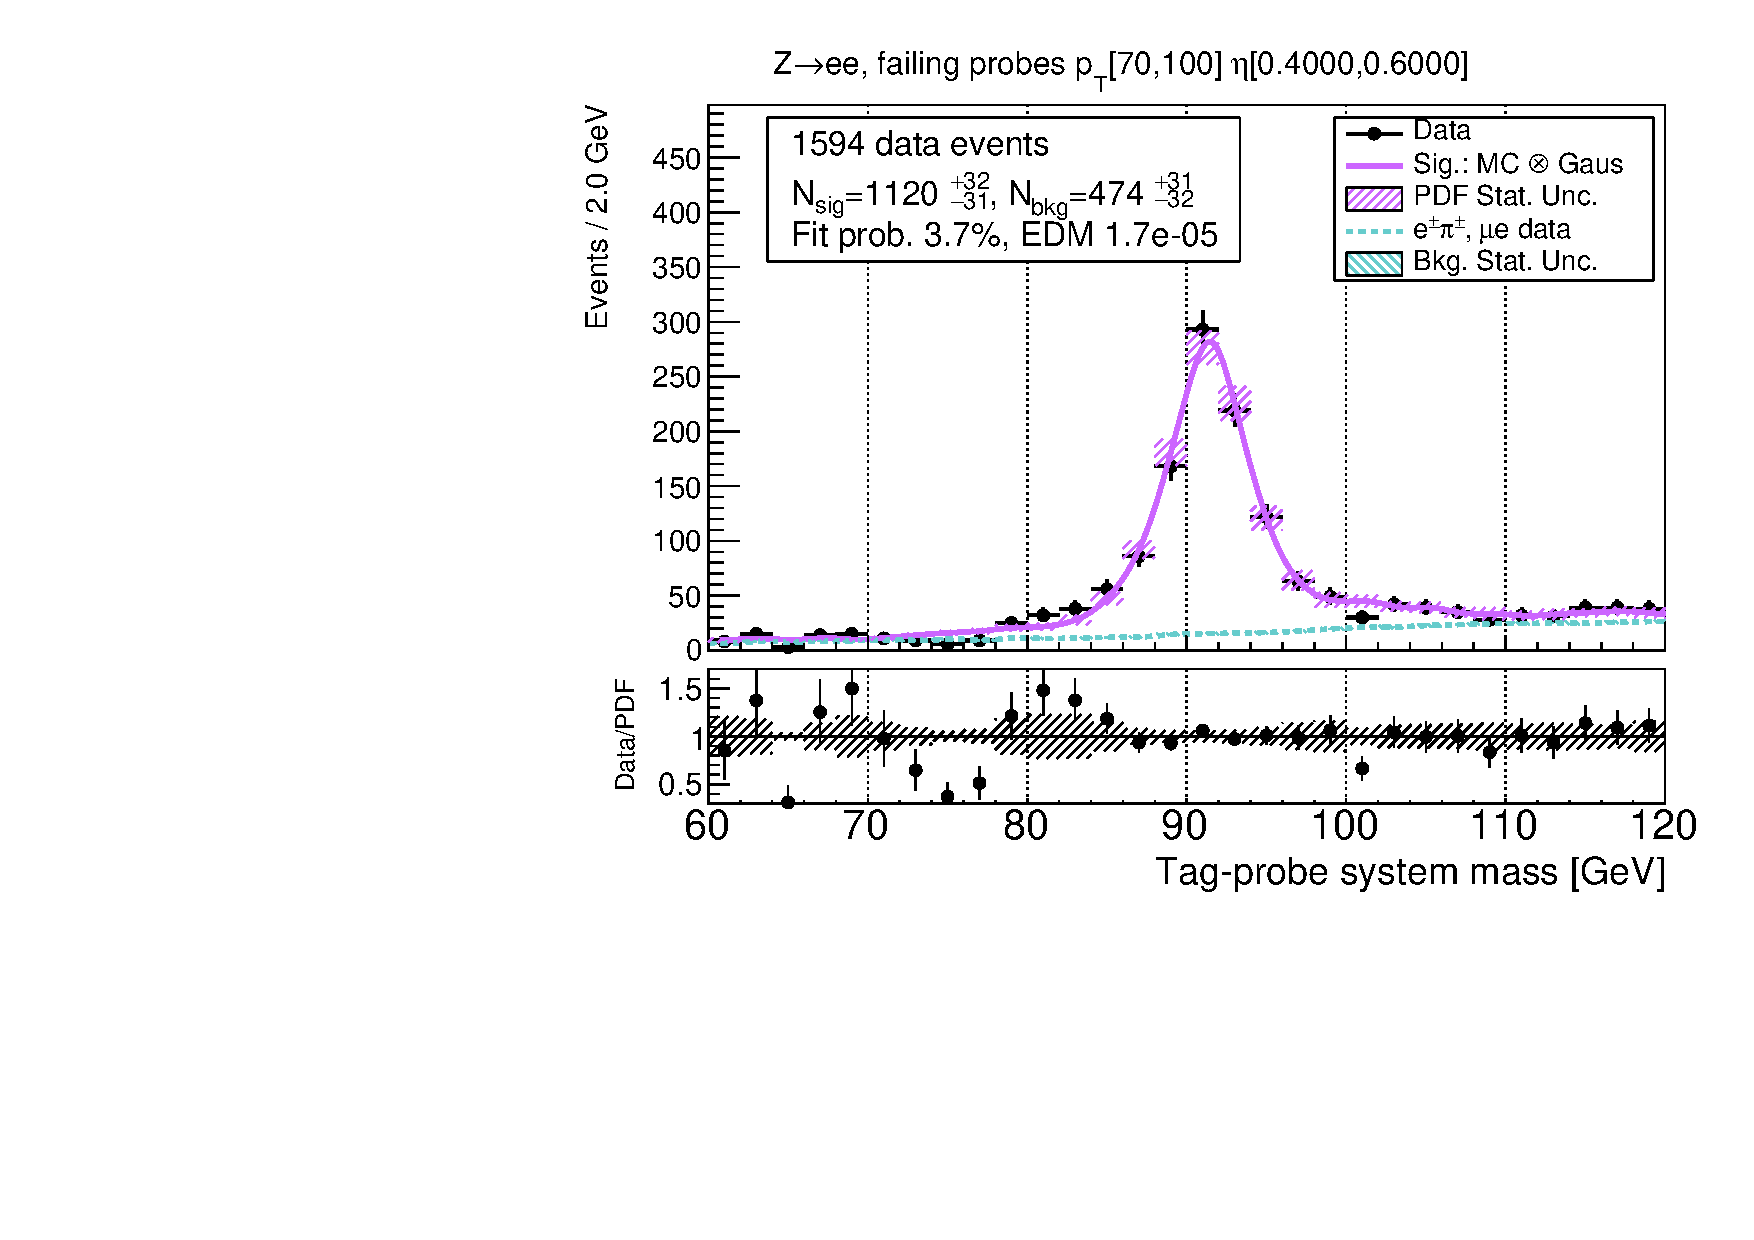
\includegraphics[width=0.49\textwidth]{figures/Zee_RecoTemplate_BkgLPiEMu_fail_ptBin14_etaBin17.pdf}
\caption{Efficiency extraction fits for the Medium electron working point using the data-driven background shape, at higher values of electron transverse momentum.}
\label{fig:ZeeNominalFits2}
\end{figure}

\section{Assessment of systematic uncertainty}
\label{sec:tnpsyst}
In this section, we quantify the systematic uncertainty arising from five distinct sources related to our ignorance
of the true signal and background shapes, the generator-related uncertainty, and possible selection bias.
In each case, the absolute difference between two alternative methods is taken as the systematic uncertainty.

\subsection{Background shape modeling}
To quantify the uncertainty in deriving the background shape from the data-driven method,
we use an analytic function as an alternative background shape.
The function chosen is a linear combination of: a decaying exponential to model low-energy fakes,
and a wide Gaussian with exponential tails to represent the peaking structure
sculpted by applying energy cuts to a falling combinatorial background mass distribution.
Previously, an error function multiplied with a decaying exponential was used, but this function
has problems related to fit convergence due to poor parameterization.

Examples of fits for 2016 run eras B to F with the analytic background are shown for dimuons in
Figures ~\ref{fig:ZmmAltBkgFits1} and~\ref{fig:ZmmAltBkgFits2}, 
and for dielectrons in Figures~\ref{fig:ZeeAltBkgFits1} and~\ref{fig:ZeeAltBkgFits2}.
These may be compared with the fits using the data-driven background shape 
in section \ref{sec:tnpfits}.
The difference in the Data/MC scale factors derived using the two methods is taken as a systematic; 
see Figures~\ref{fig:ZmmSystBkgModel} and~\ref{fig:ZeeSystBkgModel}.

\begin{figure}
\centering
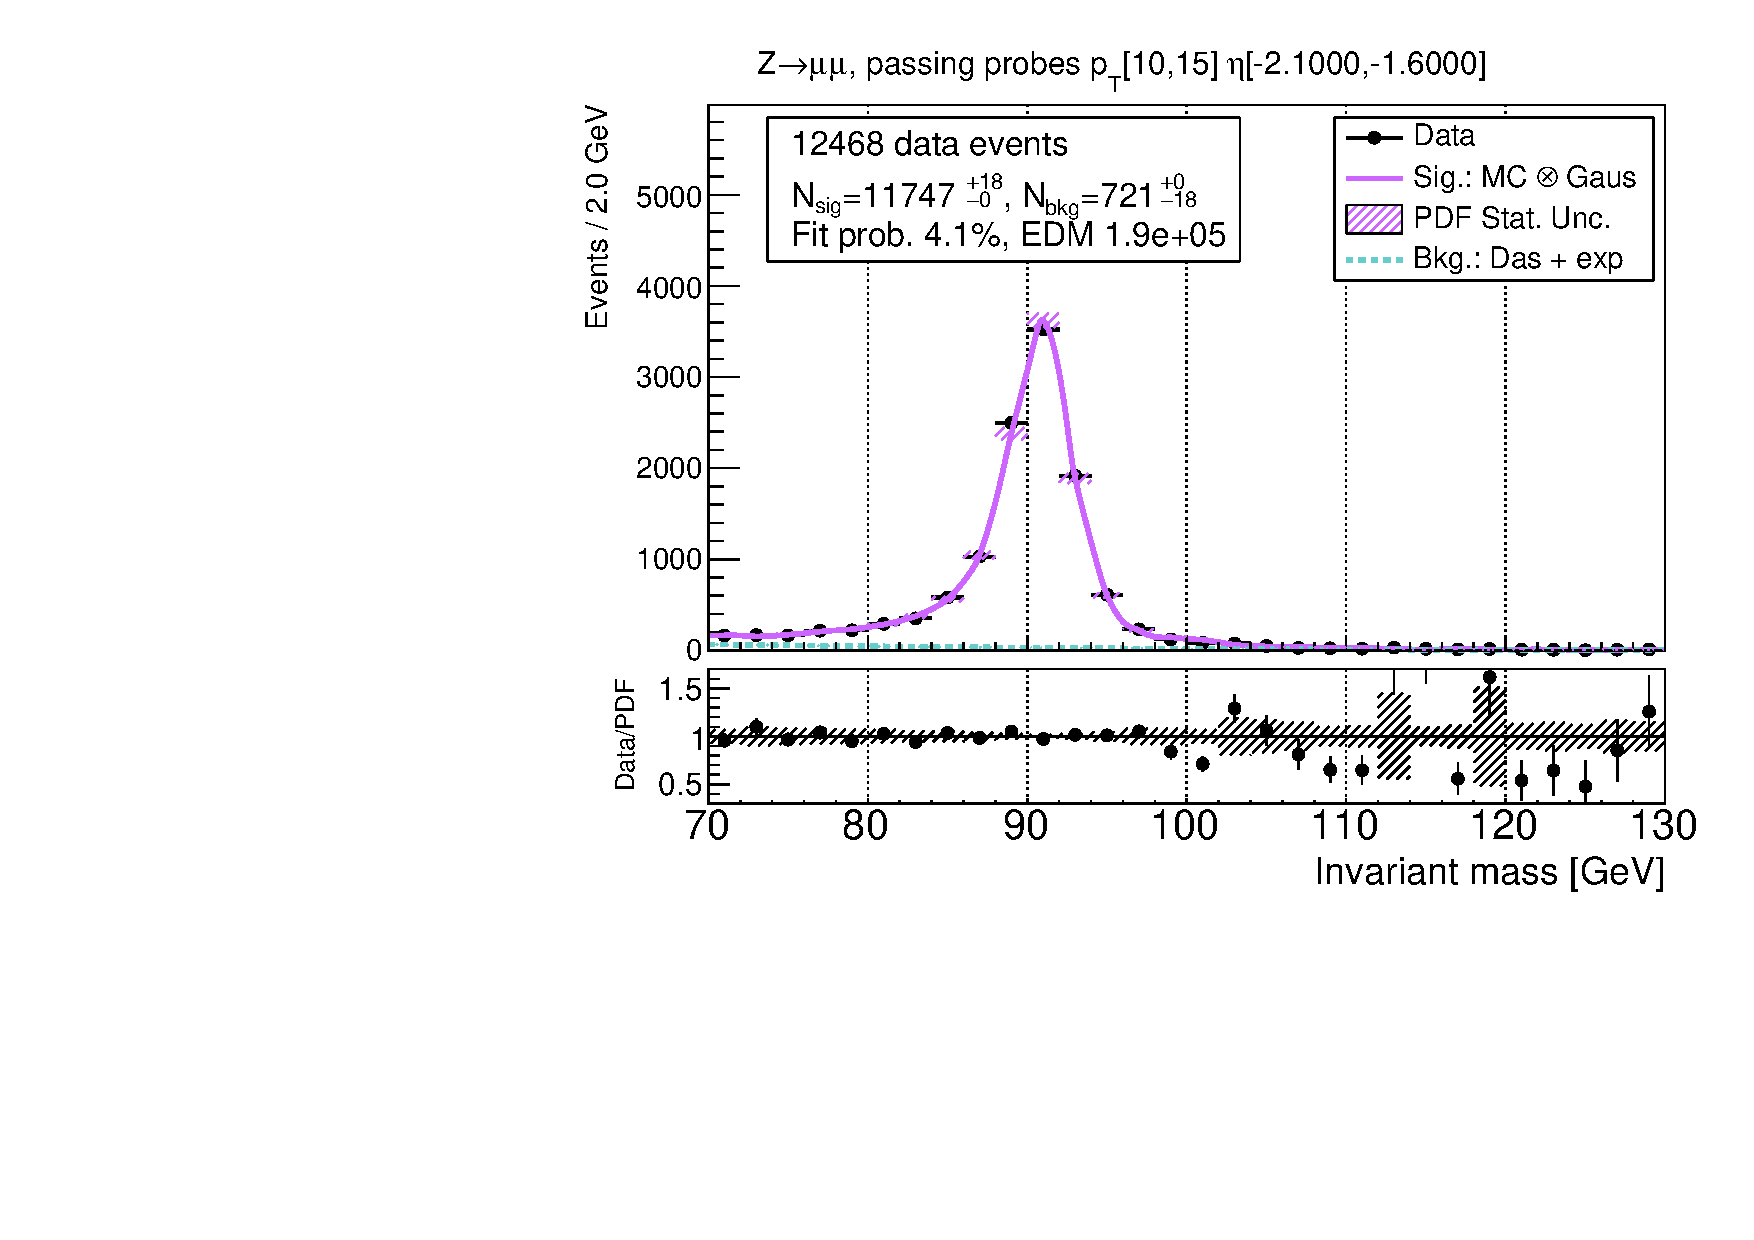
\includegraphics[width=0.49\textwidth]{figures/Zmm_RecoTemplate_BkgAnalytic_pass_ptBin0_etaBin1.pdf}
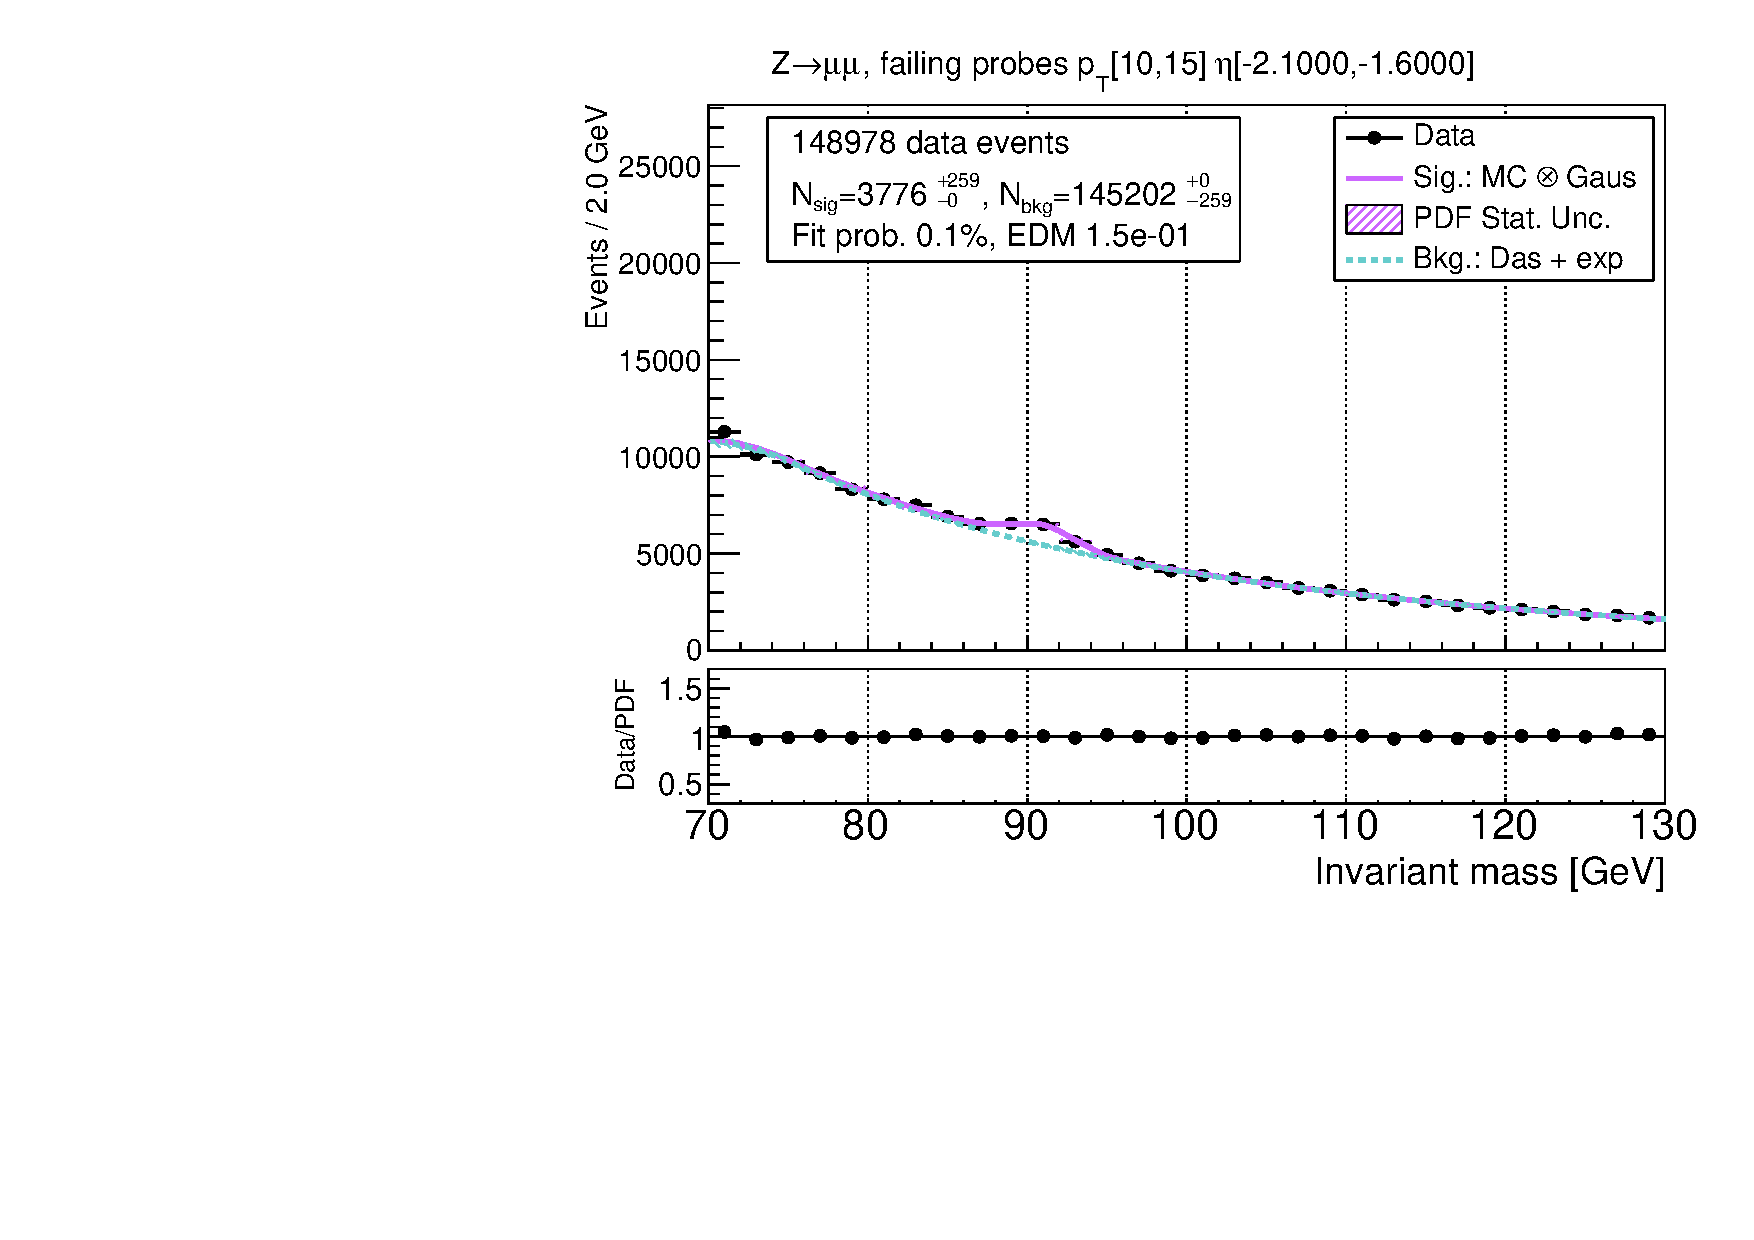
\includegraphics[width=0.49\textwidth]{figures/Zmm_RecoTemplate_BkgAnalytic_fail_ptBin0_etaBin1.pdf}
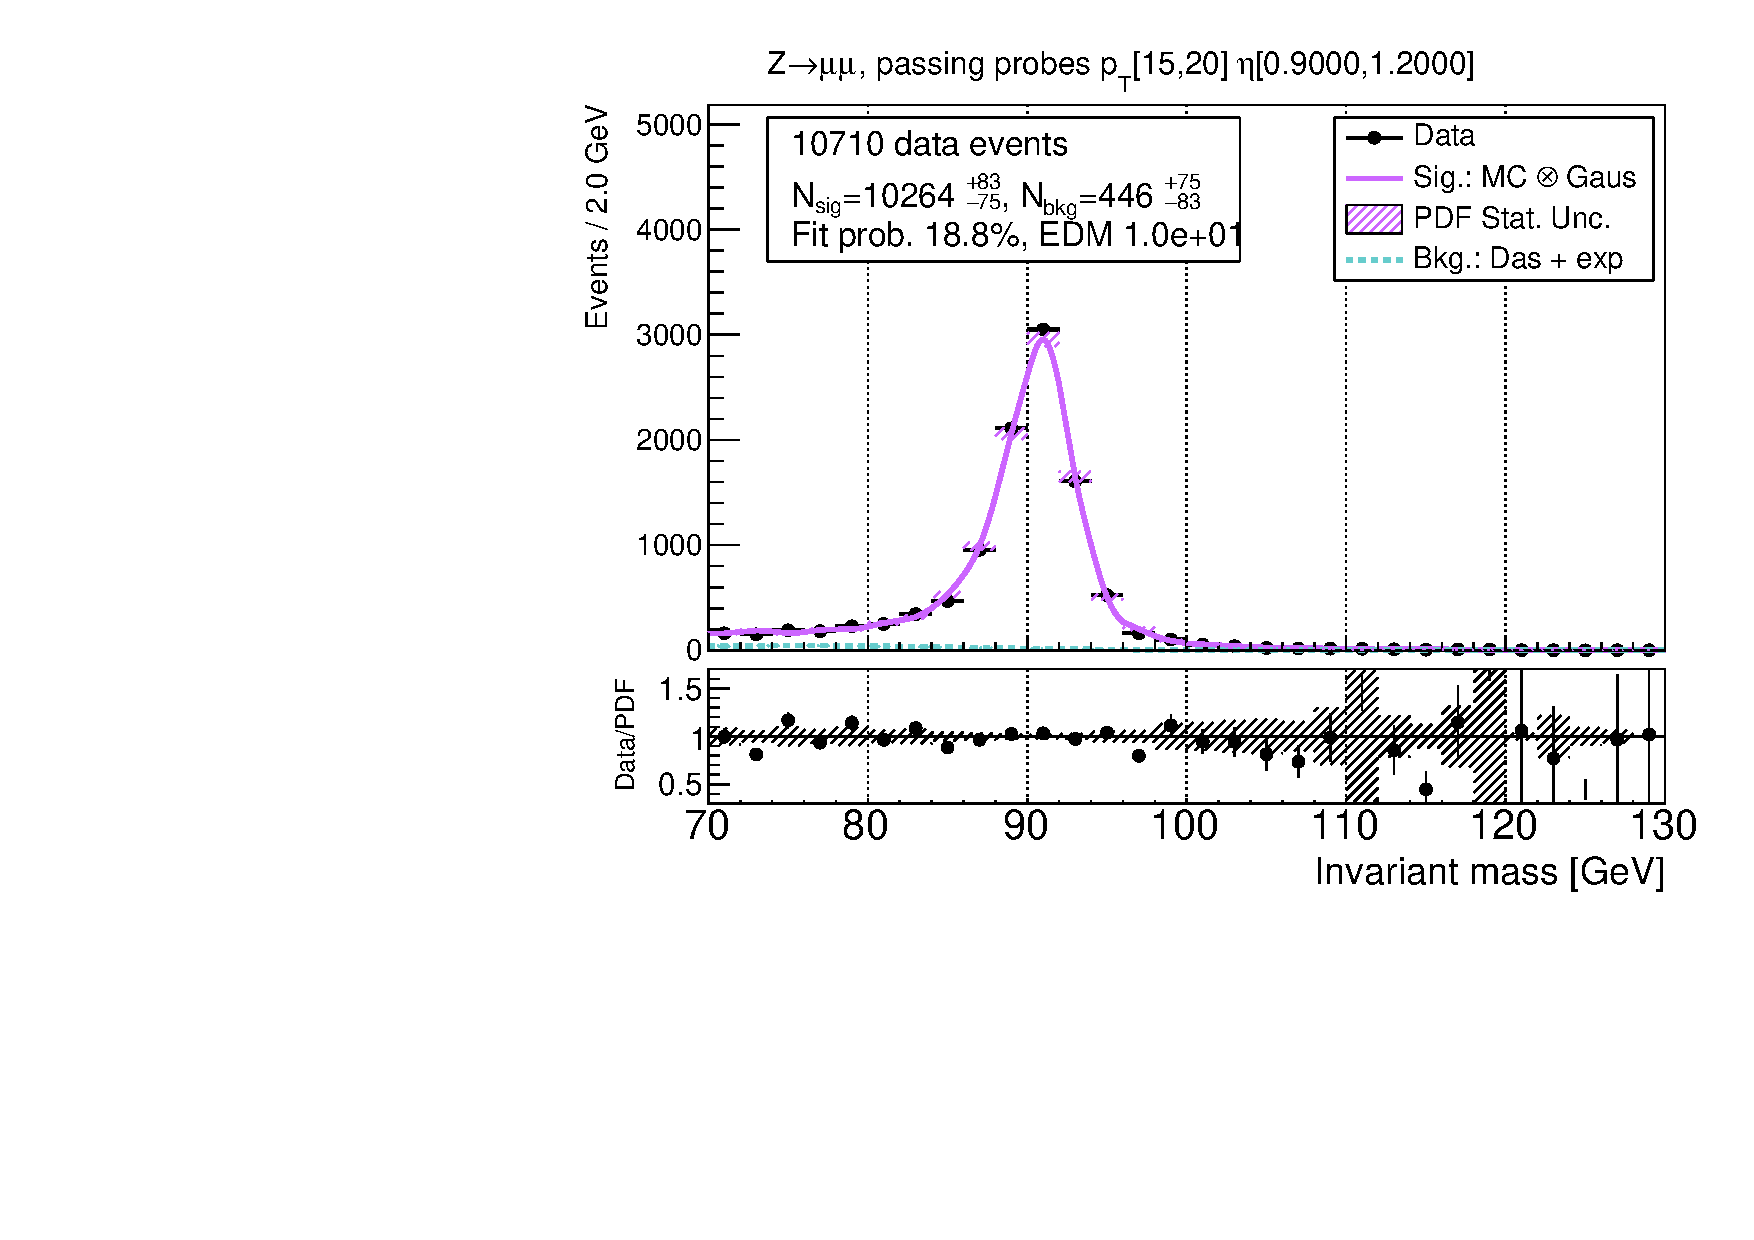
\includegraphics[width=0.49\textwidth]{figures/Zmm_RecoTemplate_BkgAnalytic_pass_ptBin1_etaBin9.pdf}
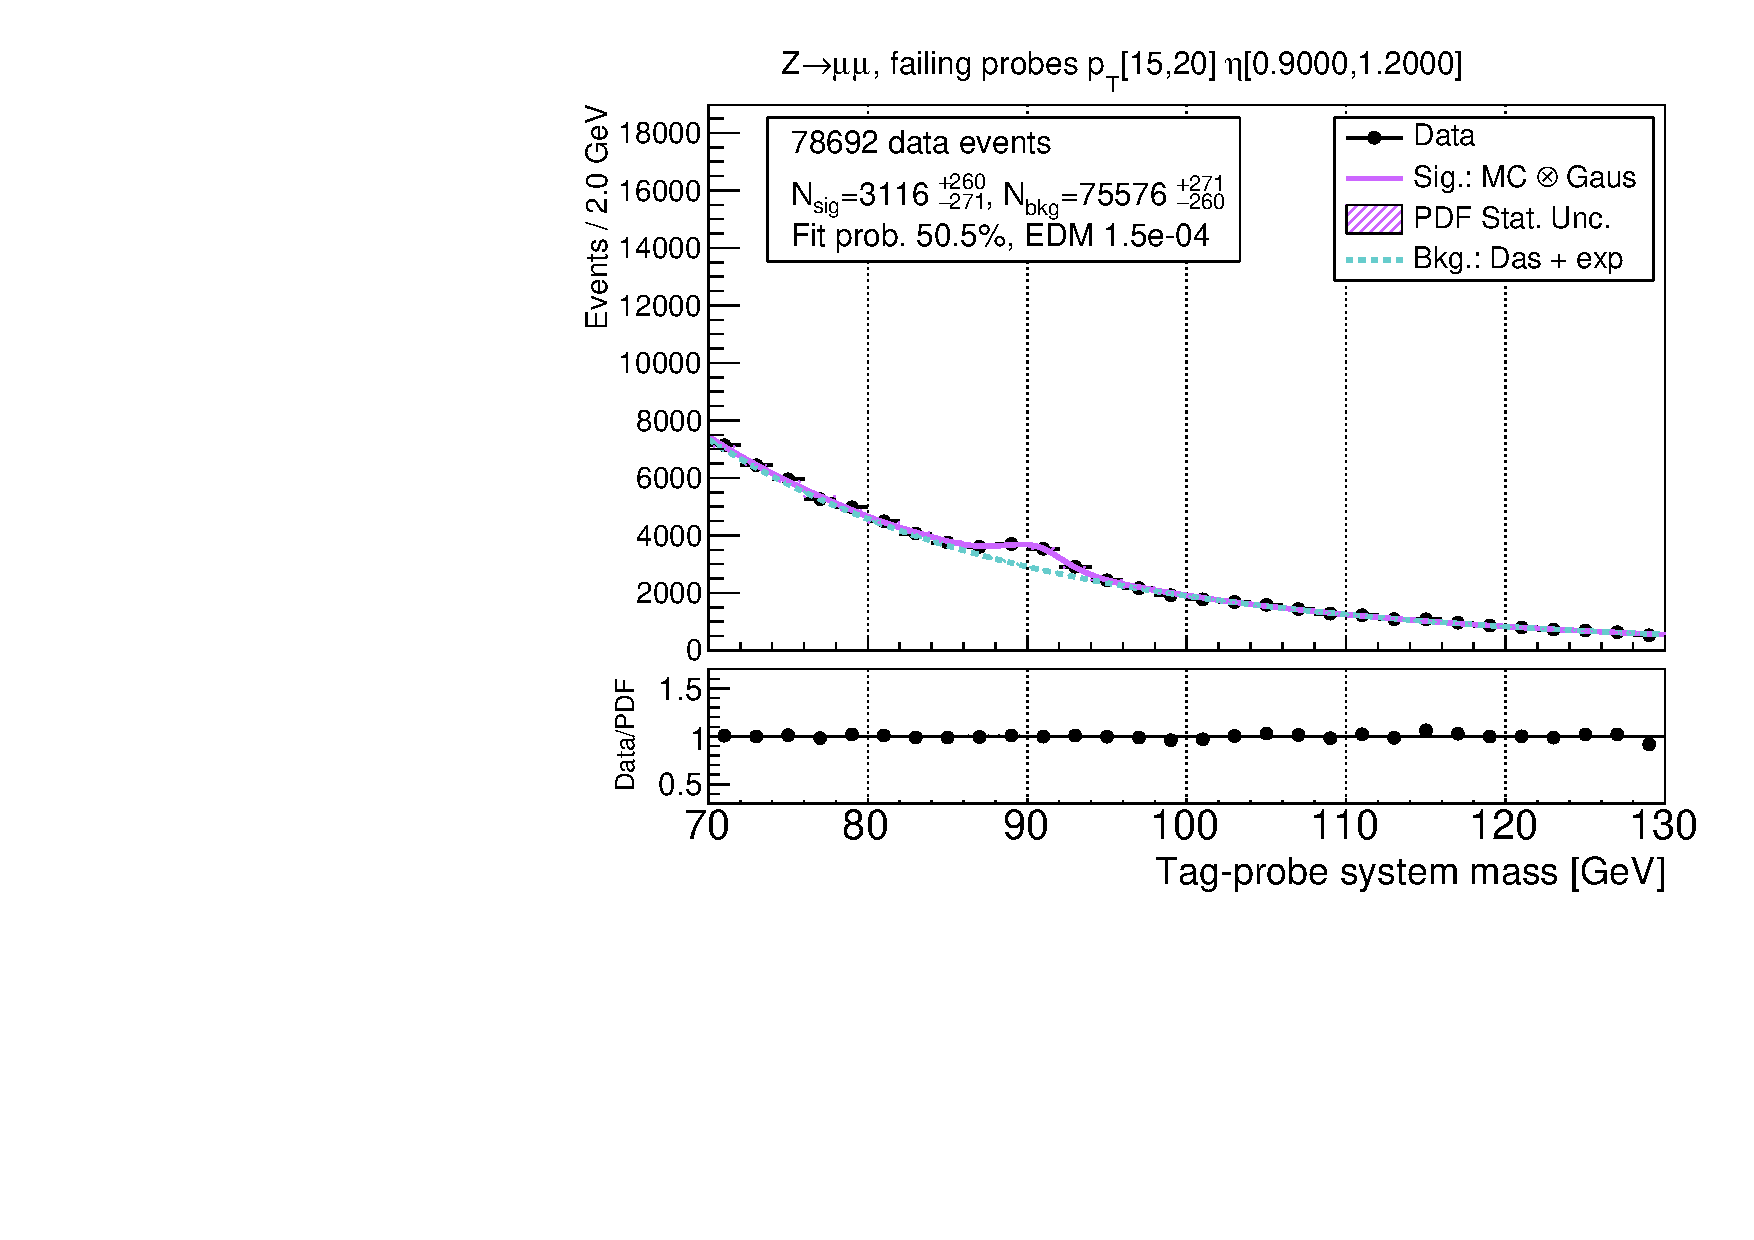
\includegraphics[width=0.49\textwidth]{figures/Zmm_RecoTemplate_BkgAnalytic_fail_ptBin1_etaBin9.pdf}
\caption{Efficiency extraction fits for the Medium muon working point using the alternative analytic background shape, at low muon transverse momentum.}
\label{fig:ZmmAltBkgFits1}
\end{figure}

\begin{figure}
\centering
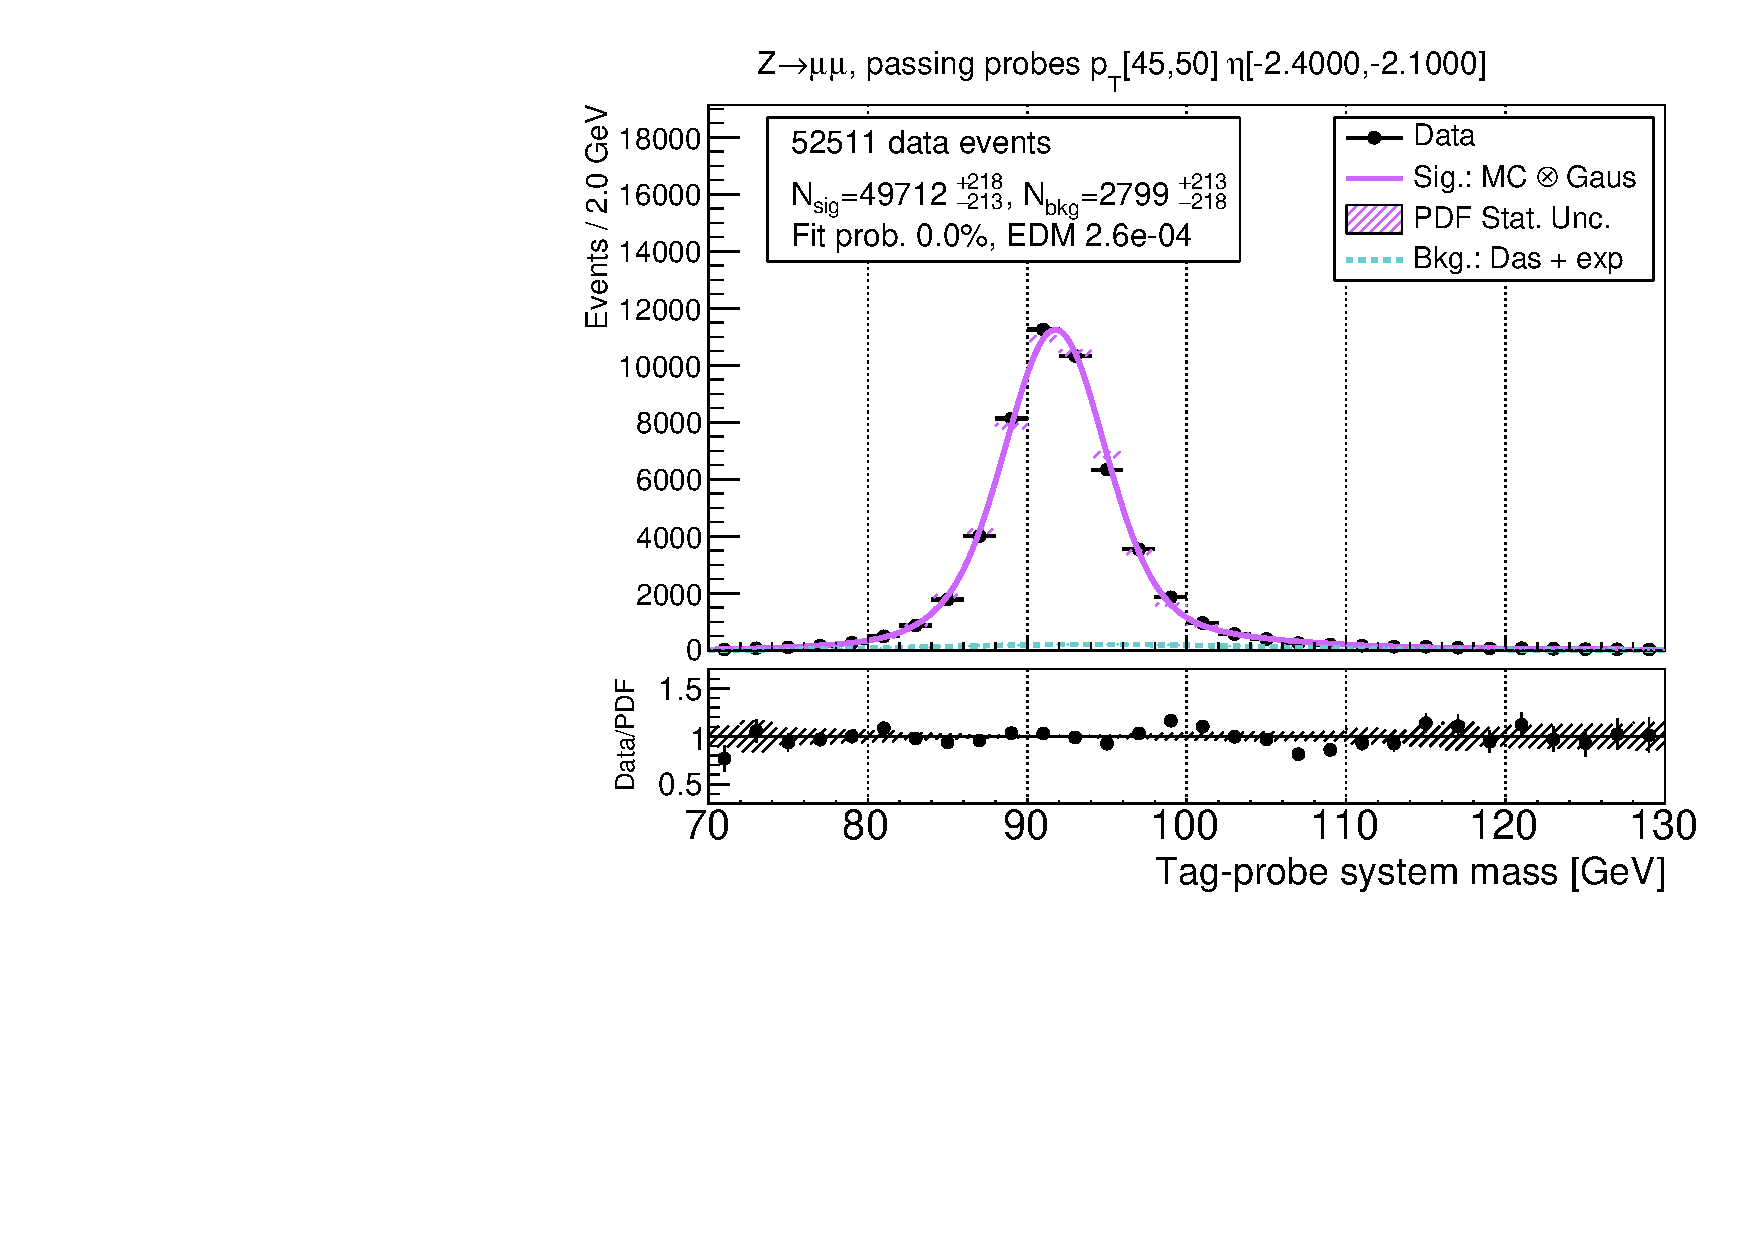
\includegraphics[width=0.49\textwidth]{figures/Zmm_RecoTemplate_BkgAnalytic_pass_ptBin7_etaBin0.pdf}
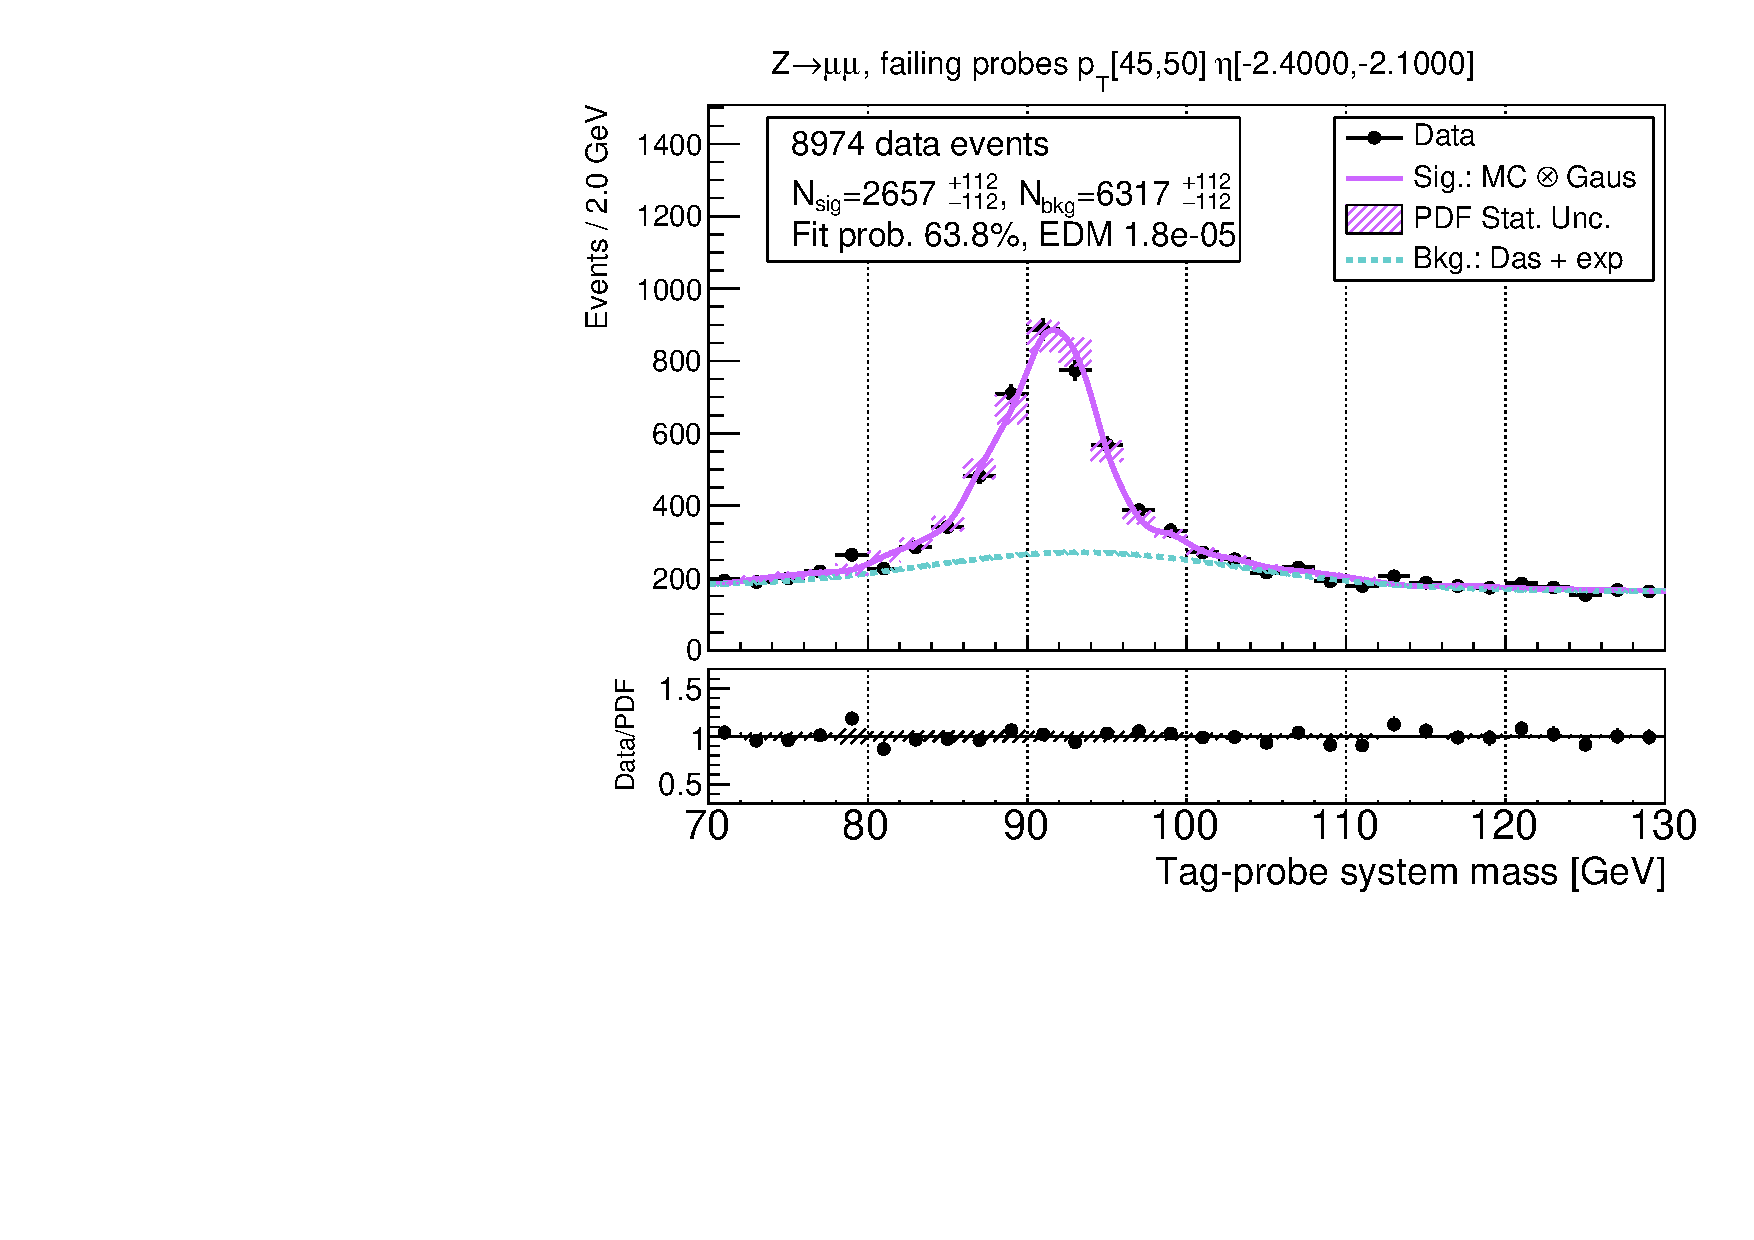
\includegraphics[width=0.49\textwidth]{figures/Zmm_RecoTemplate_BkgAnalytic_fail_ptBin7_etaBin0.pdf}
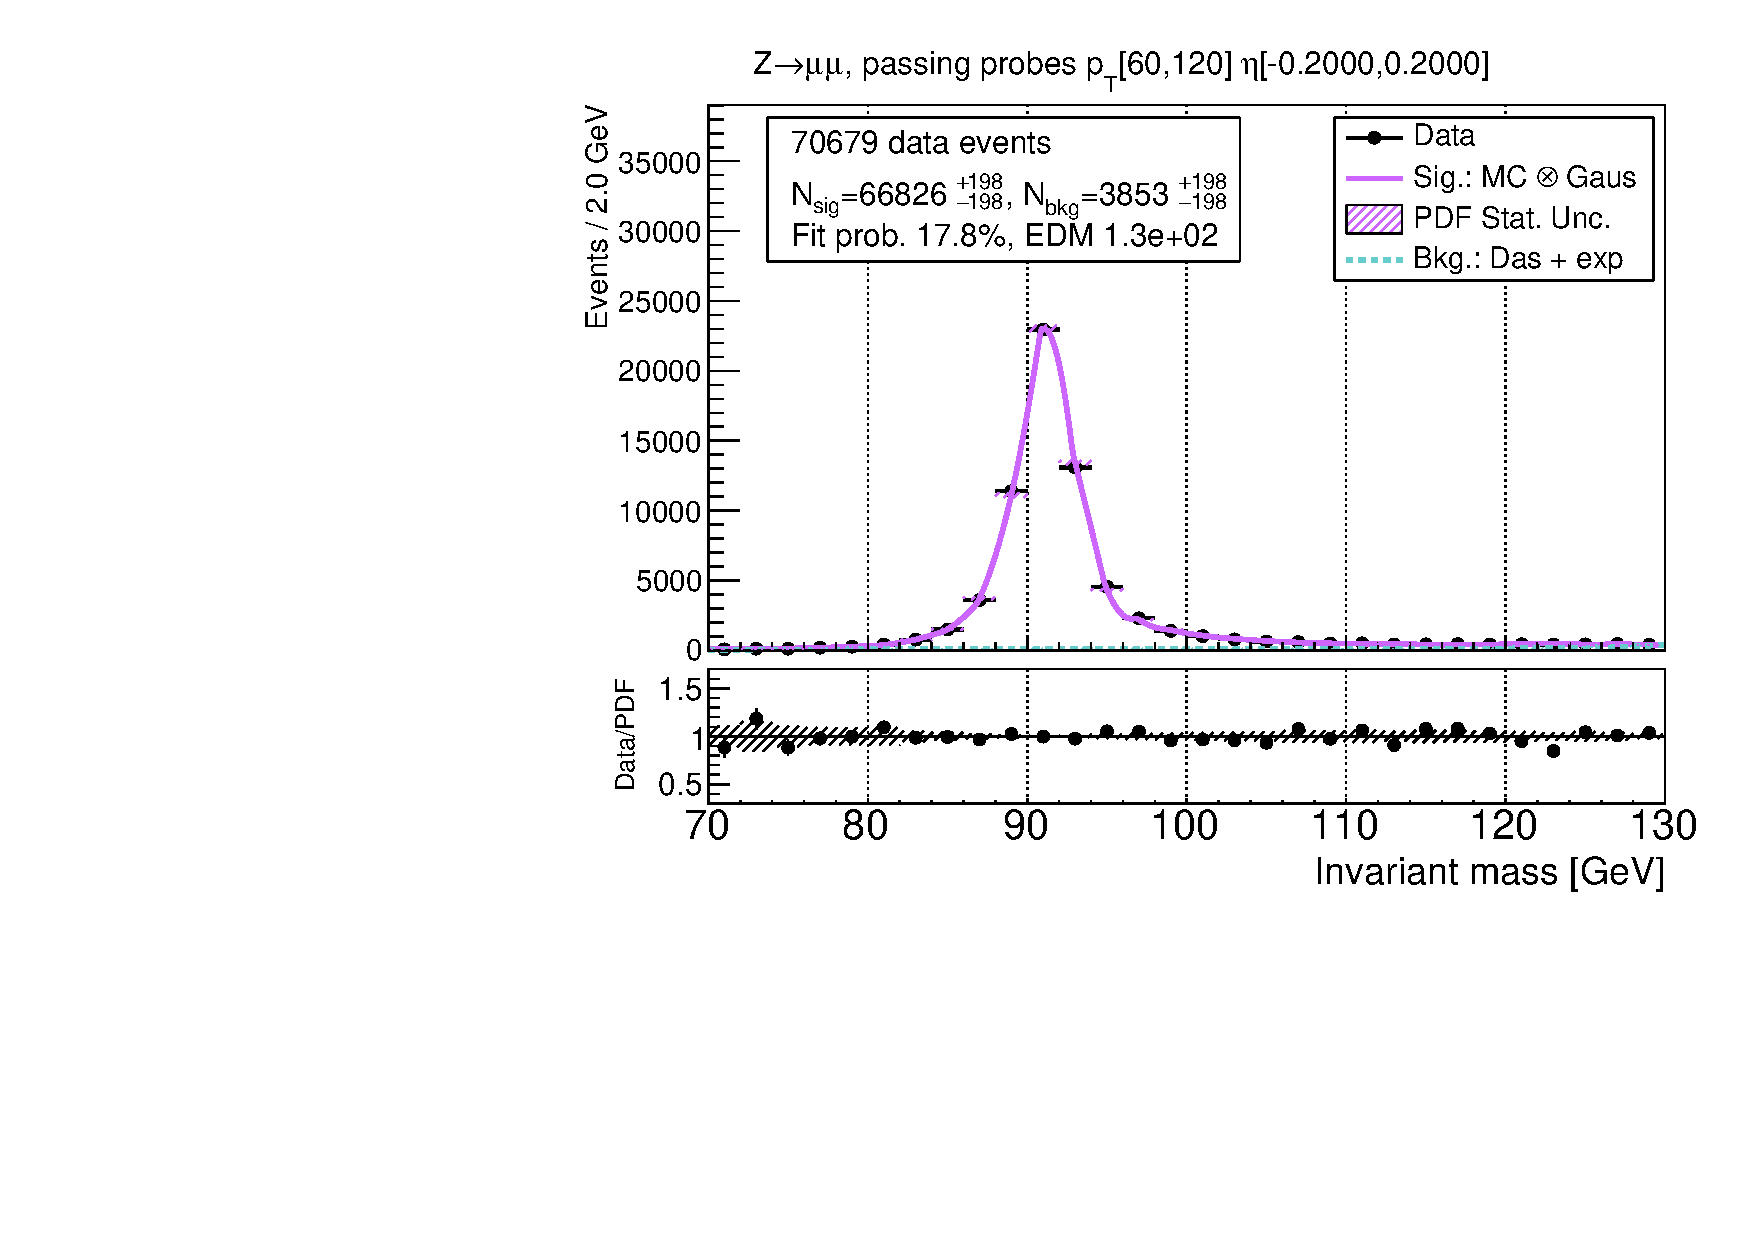
\includegraphics[width=0.49\textwidth]{figures/Zmm_RecoTemplate_BkgAnalytic_pass_ptBin10_etaBin6.pdf}
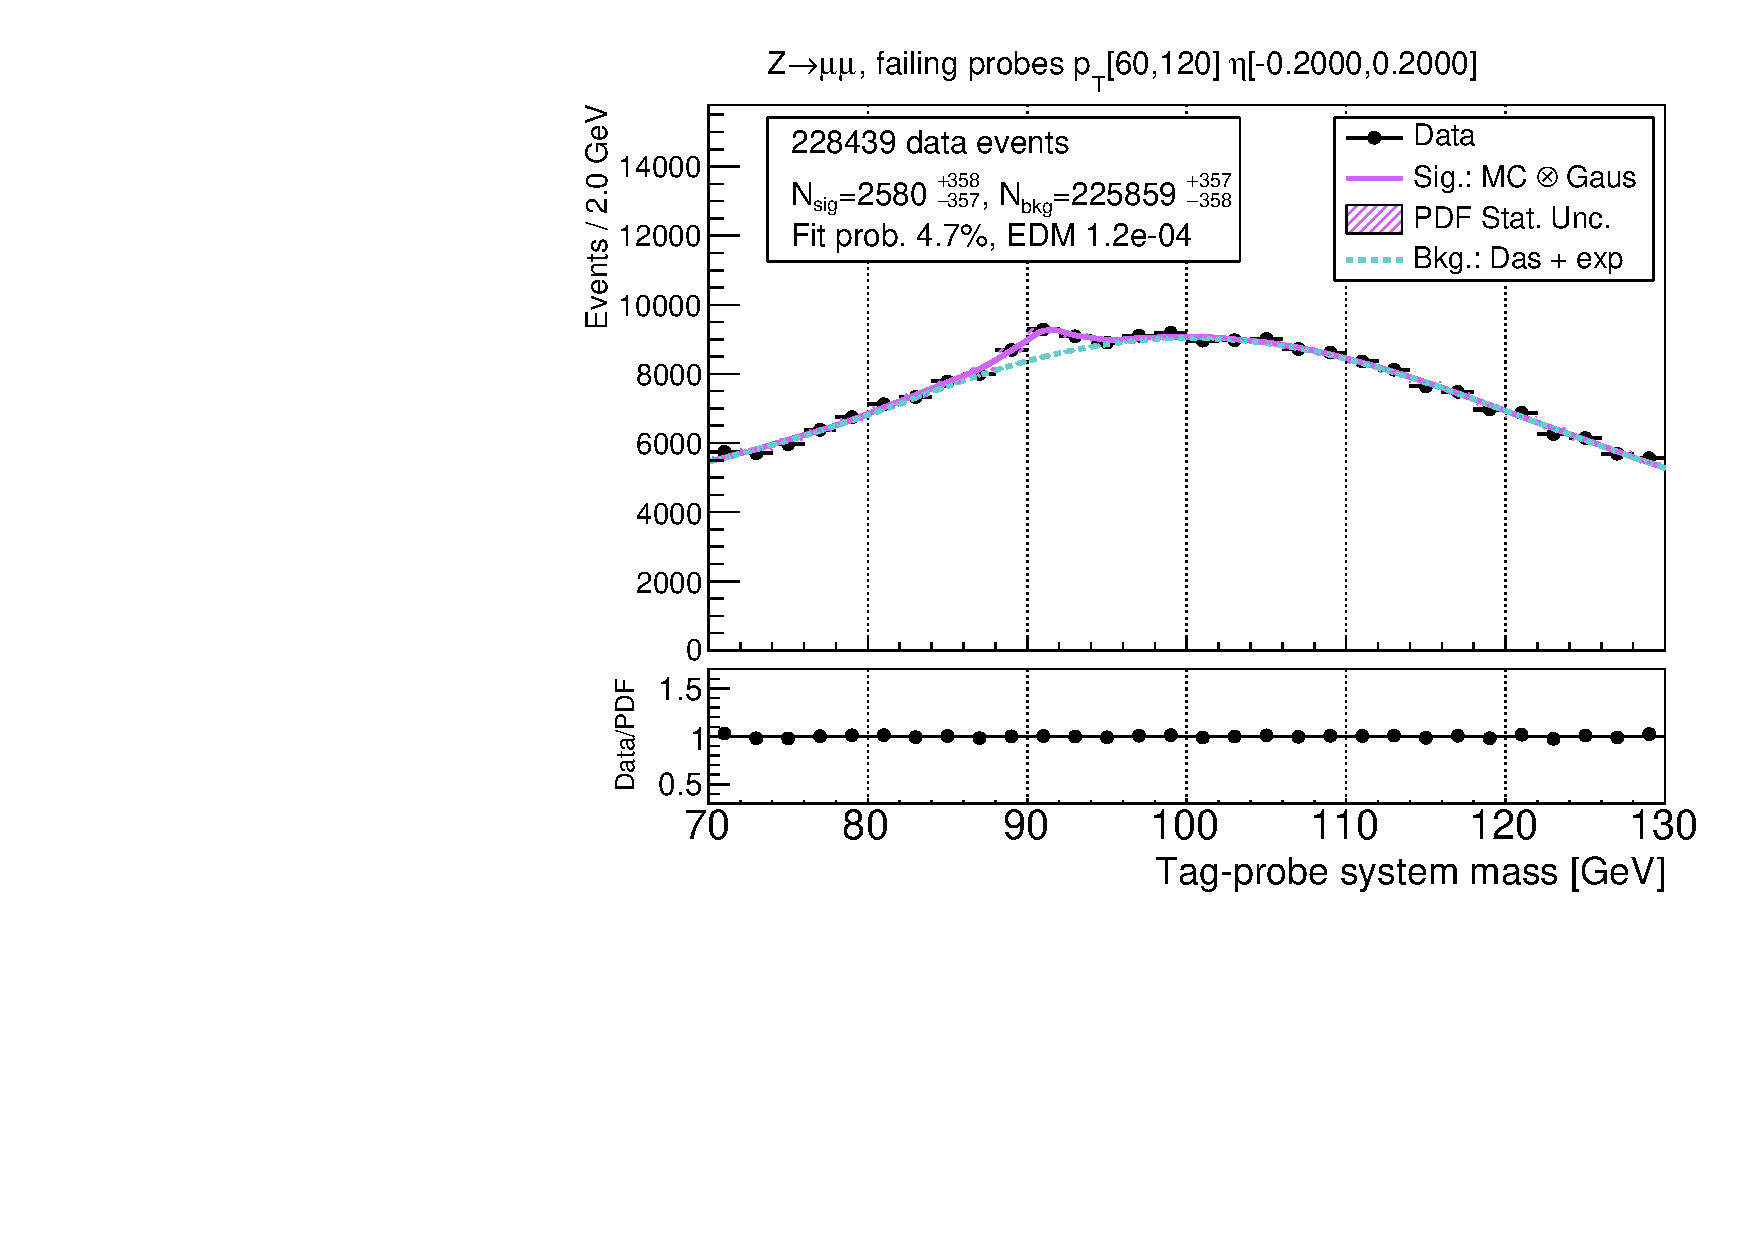
\includegraphics[width=0.49\textwidth]{figures/Zmm_RecoTemplate_BkgAnalytic_fail_ptBin10_etaBin6.pdf}
\caption{Efficiency extraction fits for the Medium muon working point using the alternative analytic background shape, at higher values of muon transverse momentum.}
\label{fig:ZmmAltBkgFits2}
\end{figure}

\begin{figure}
\centering
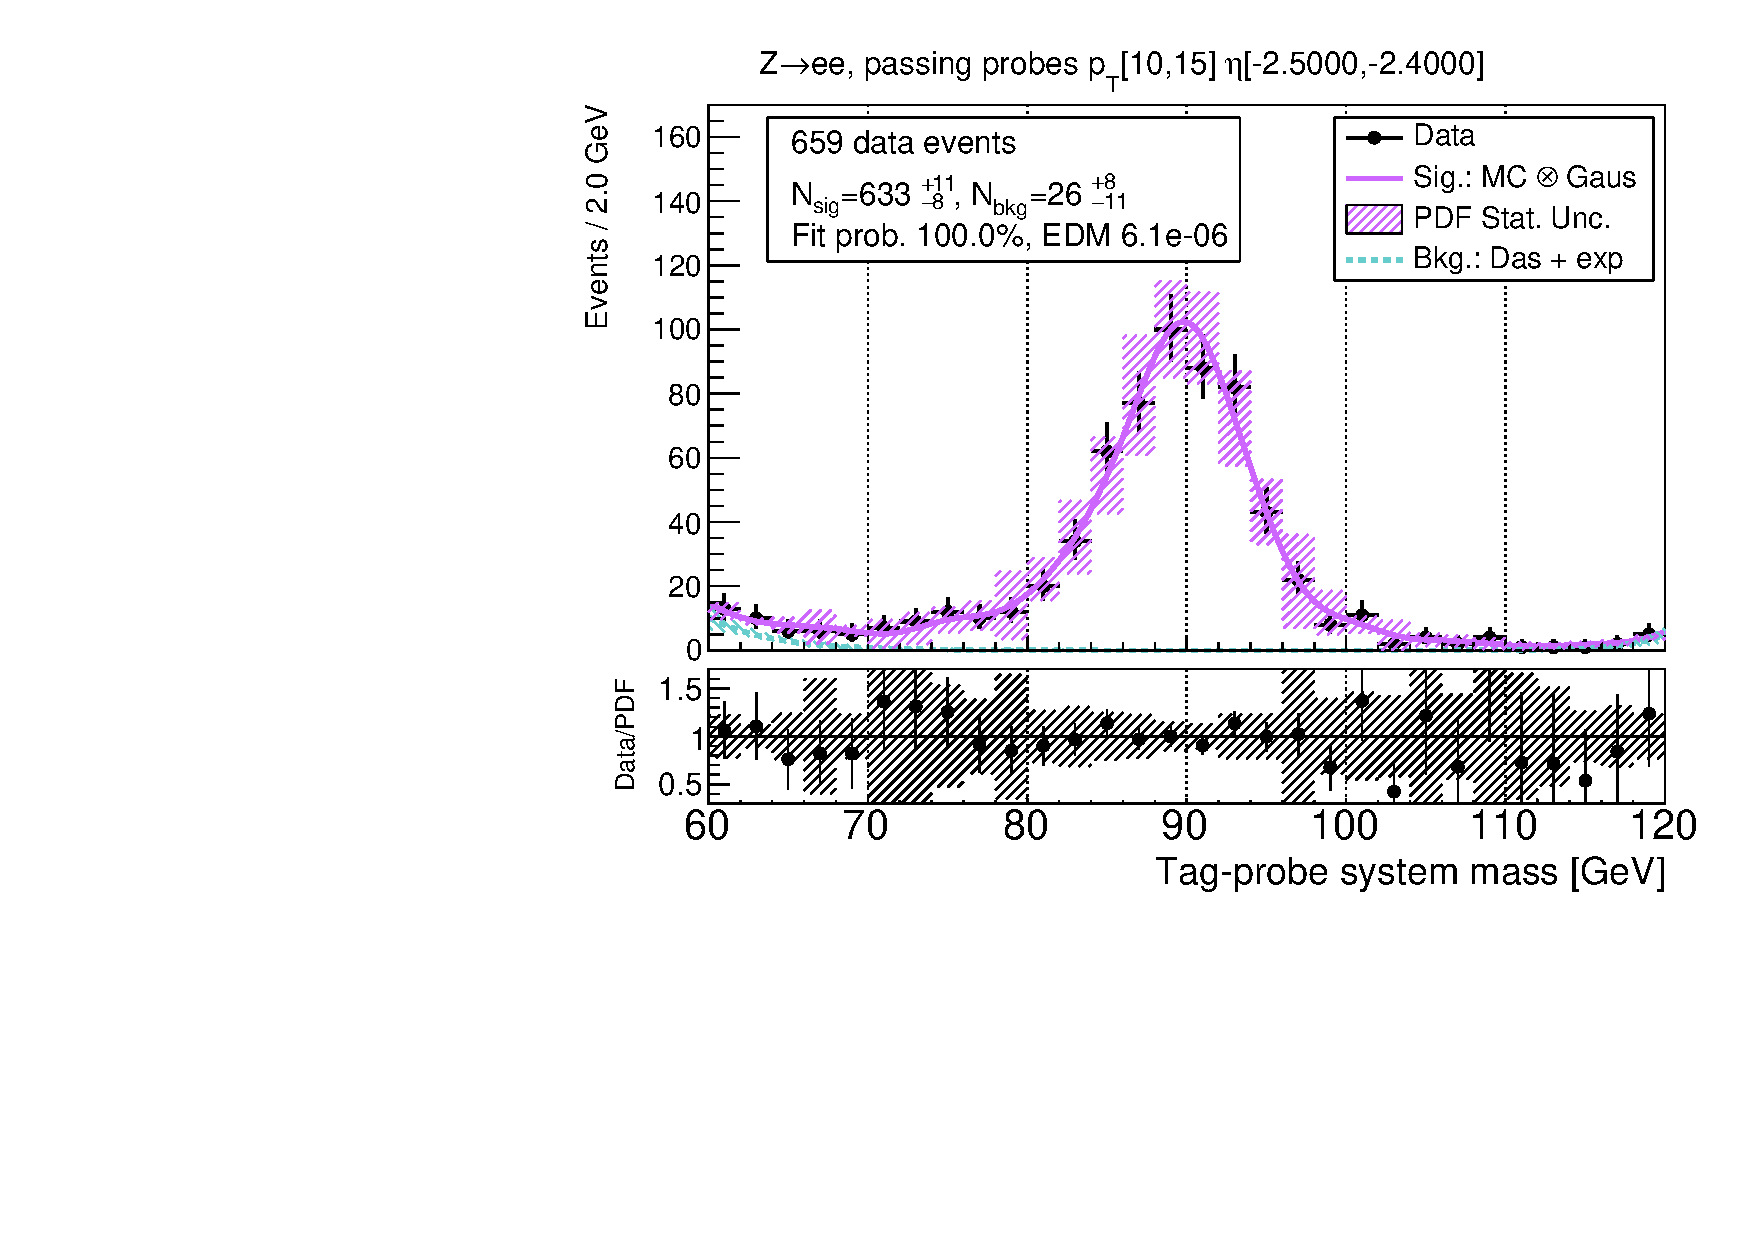
\includegraphics[width=0.49\textwidth]{figures/Zee_RecoTemplate_BkgAnalytic_pass_ptBin0_etaBin0.pdf}
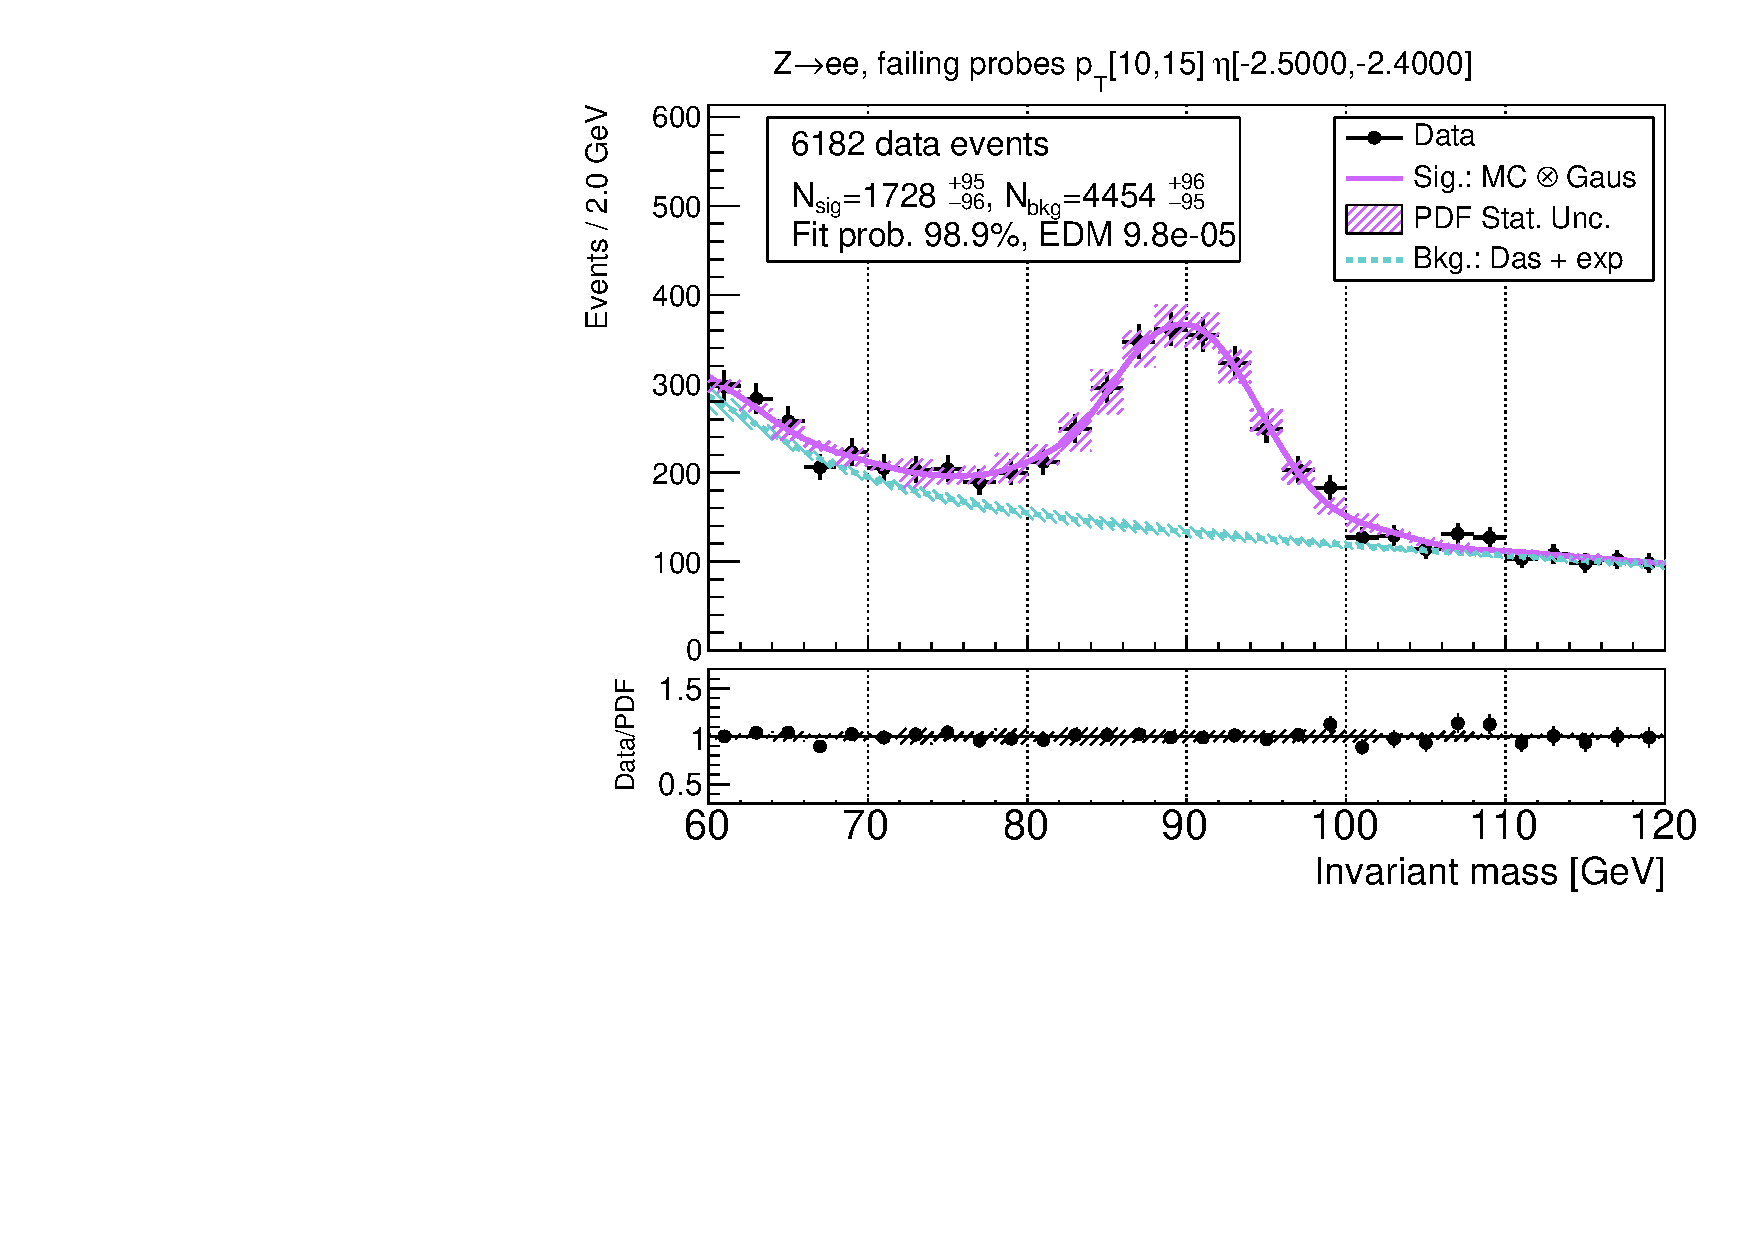
\includegraphics[width=0.49\textwidth]{figures/Zee_RecoTemplate_BkgAnalytic_fail_ptBin0_etaBin0.pdf}
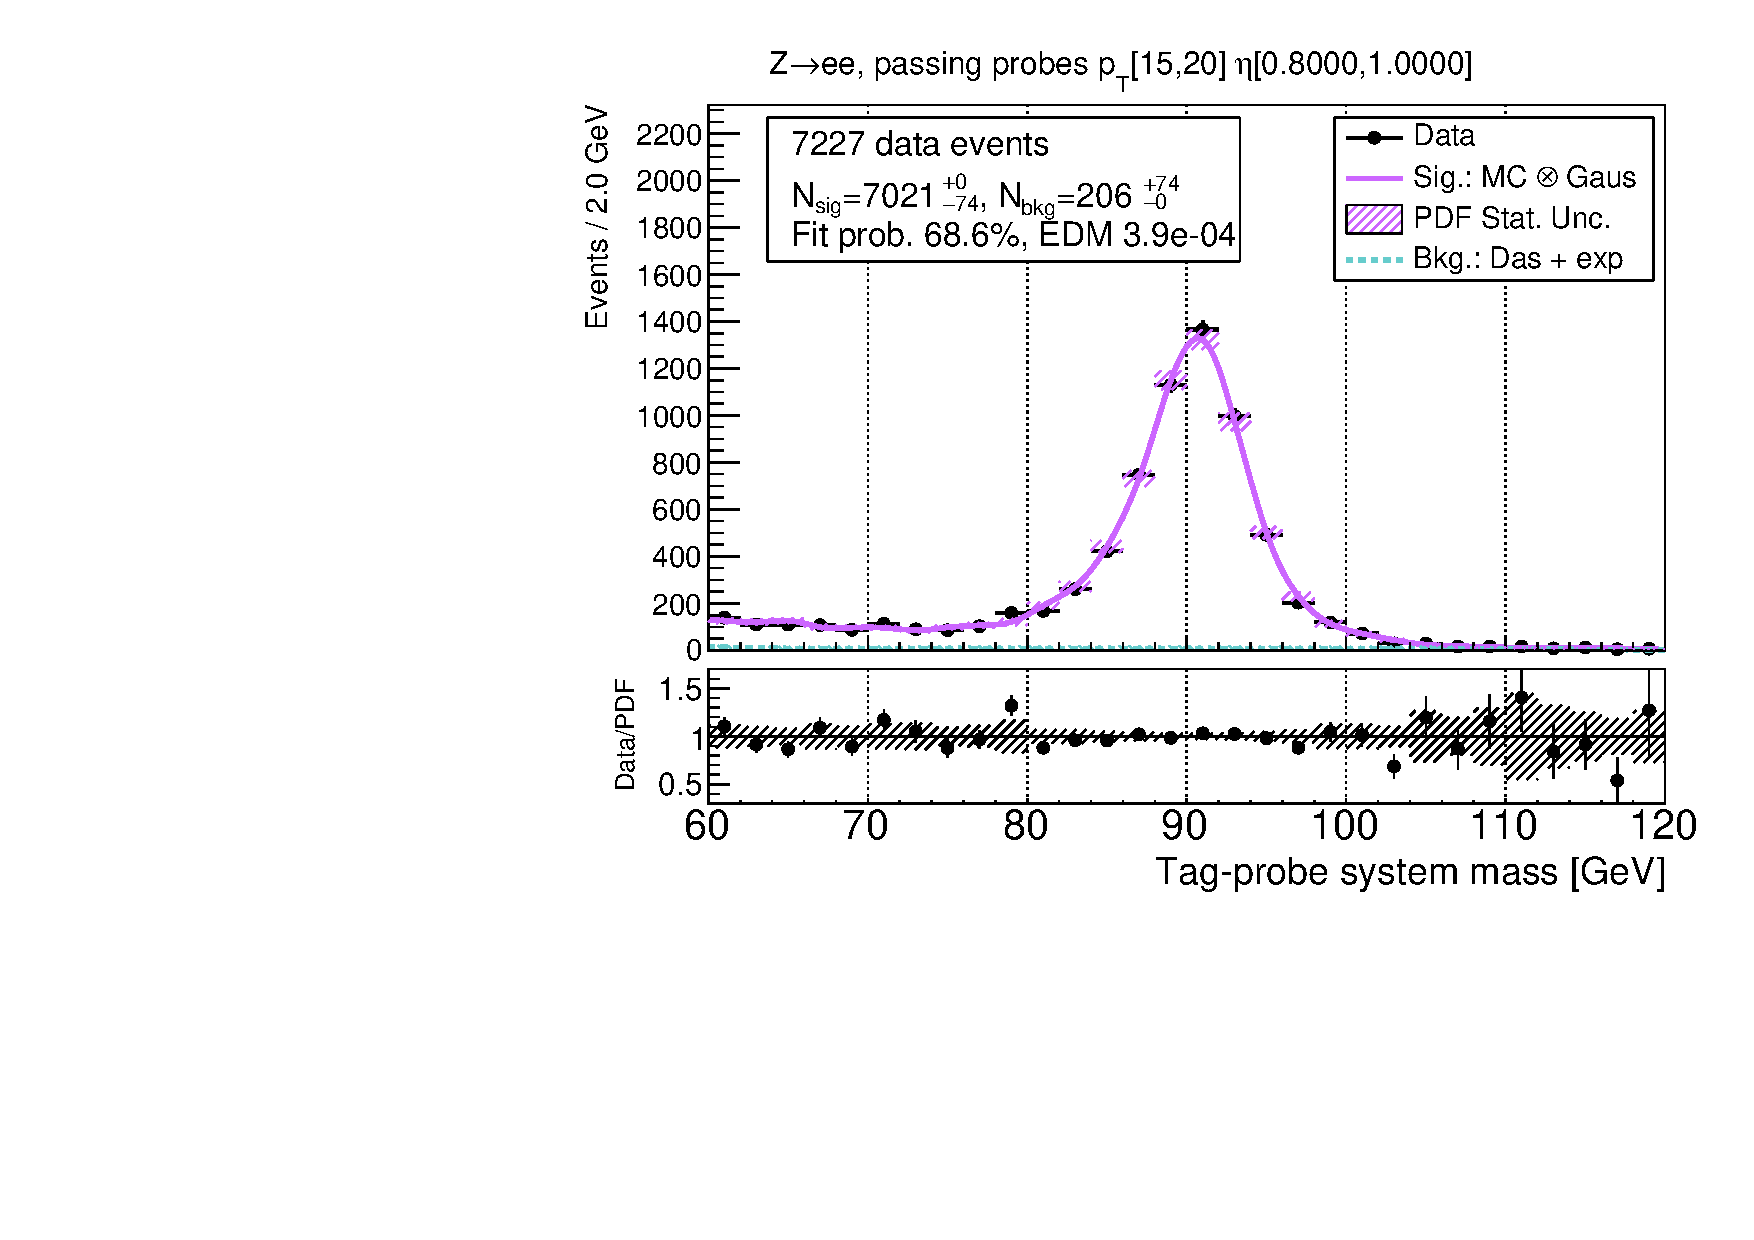
\includegraphics[width=0.49\textwidth]{figures/Zee_RecoTemplate_BkgAnalytic_pass_ptBin1_etaBin19.pdf}
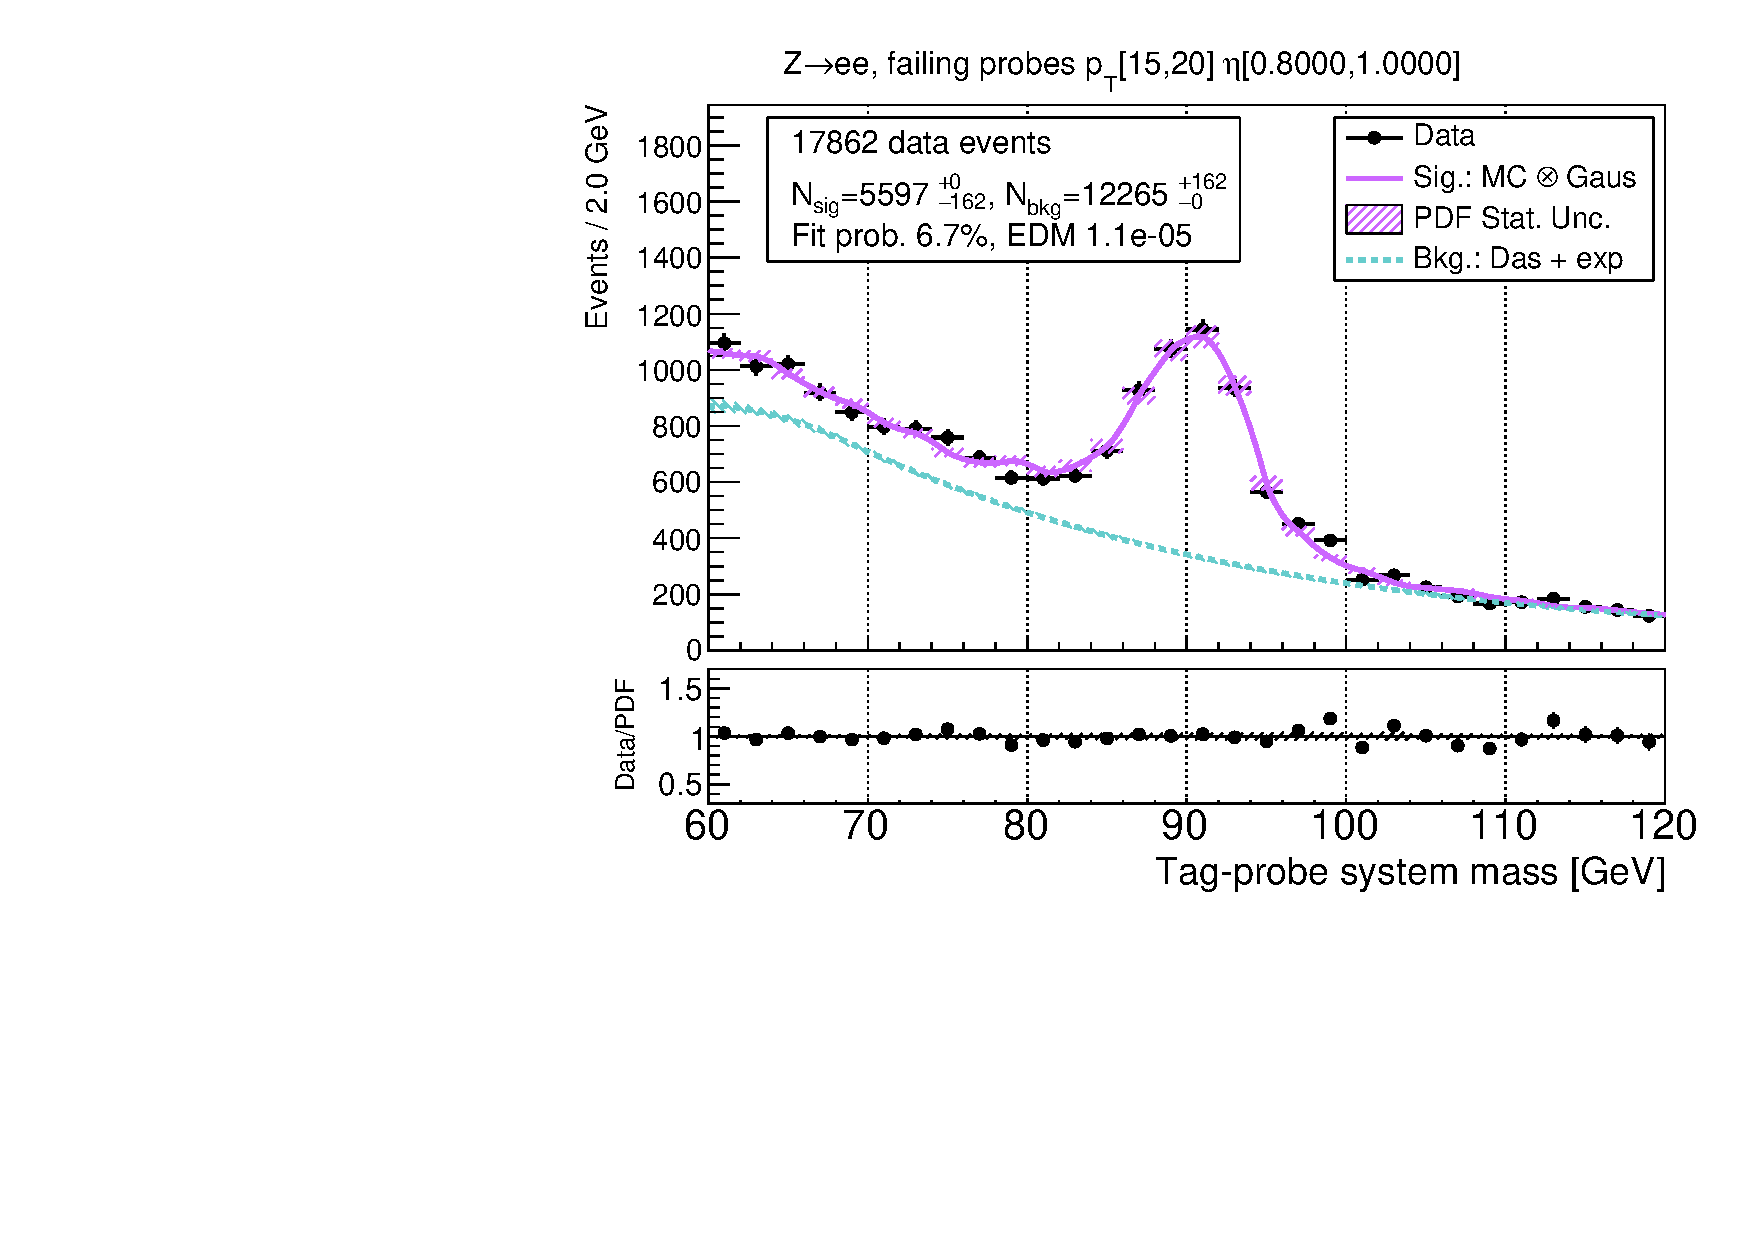
\includegraphics[width=0.49\textwidth]{figures/Zee_RecoTemplate_BkgAnalytic_fail_ptBin1_etaBin19.pdf}
\caption{Efficiency extraction fits for the Medium electron working point using the alternative analytic background shape, at low electron transverse momentum.}
\label{fig:ZeeAltBkgFits1}
\end{figure}

\begin{figure}
\centering
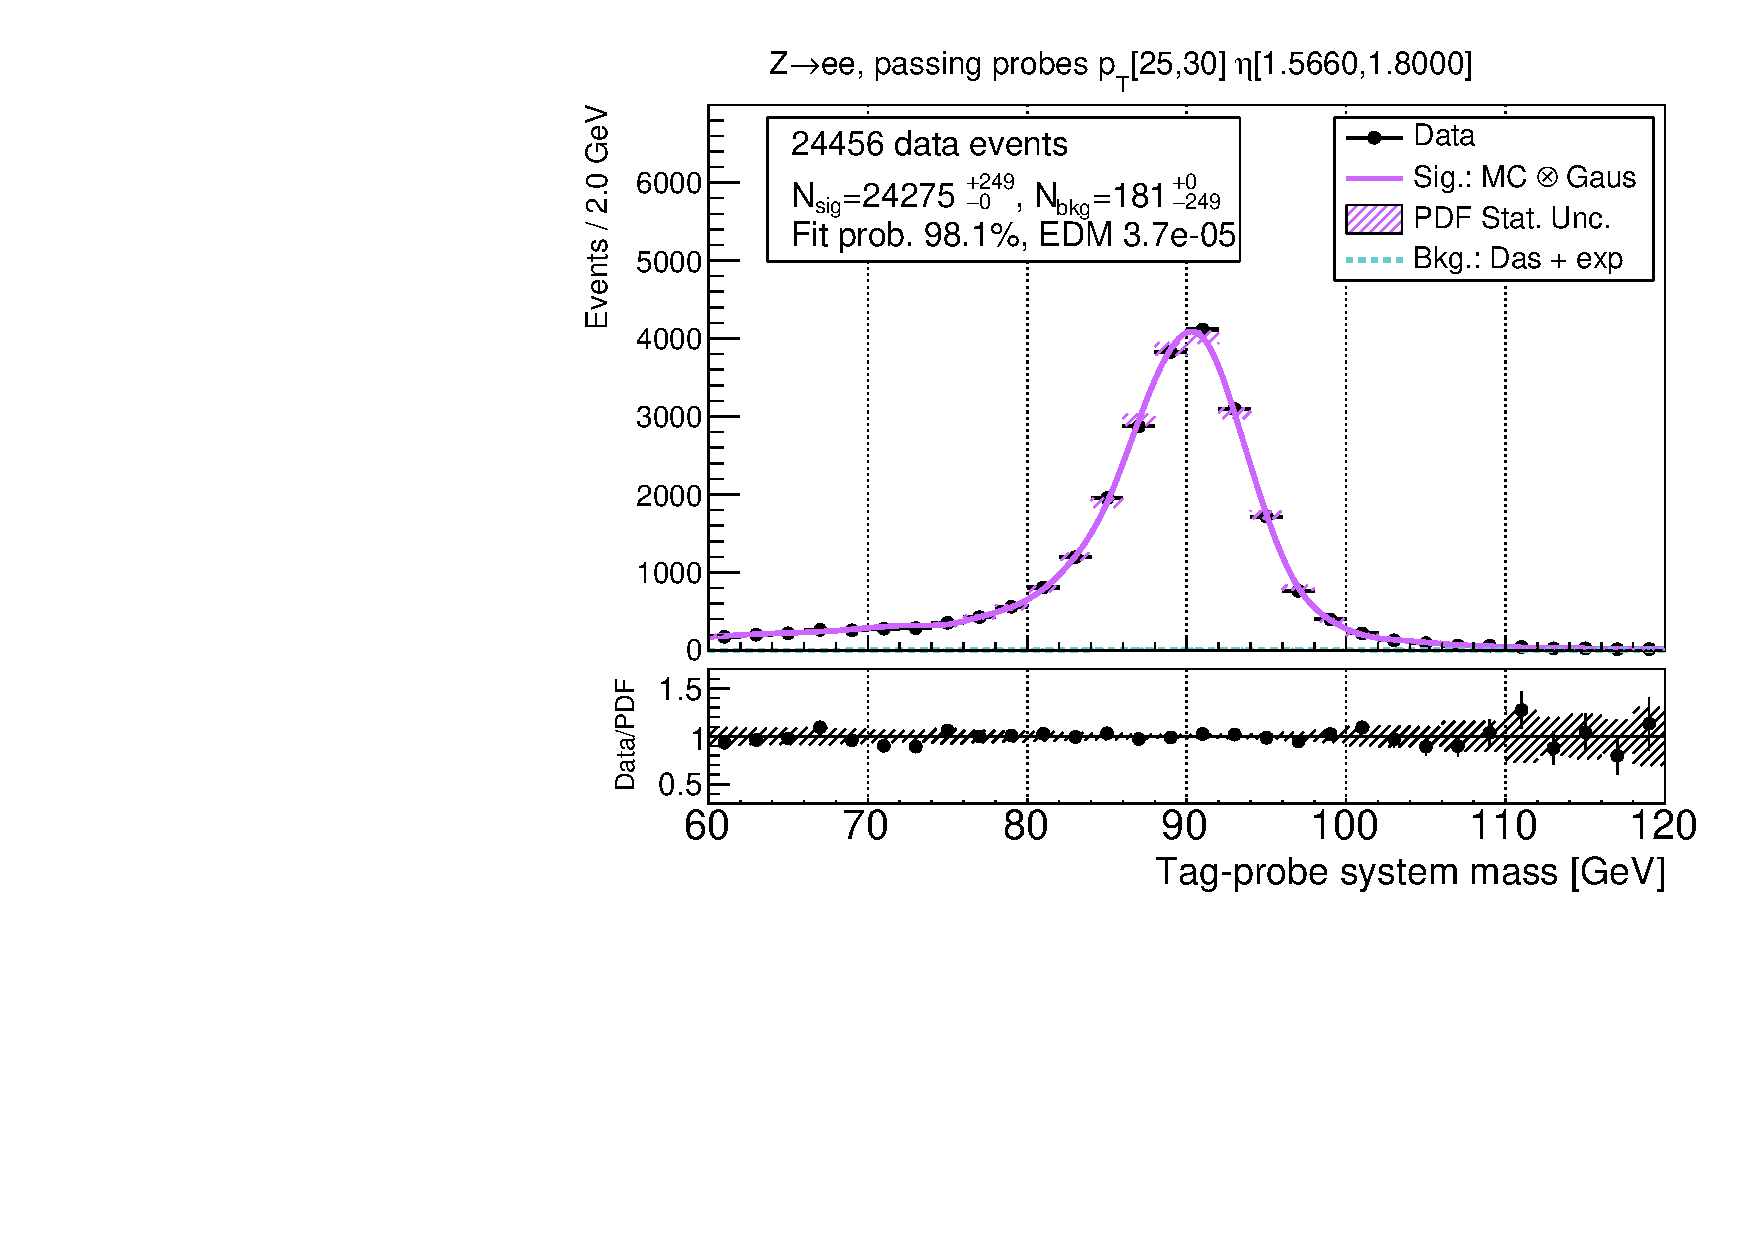
\includegraphics[width=0.49\textwidth]{figures/Zee_RecoTemplate_BkgAnalytic_pass_ptBin3_etaBin23.pdf}
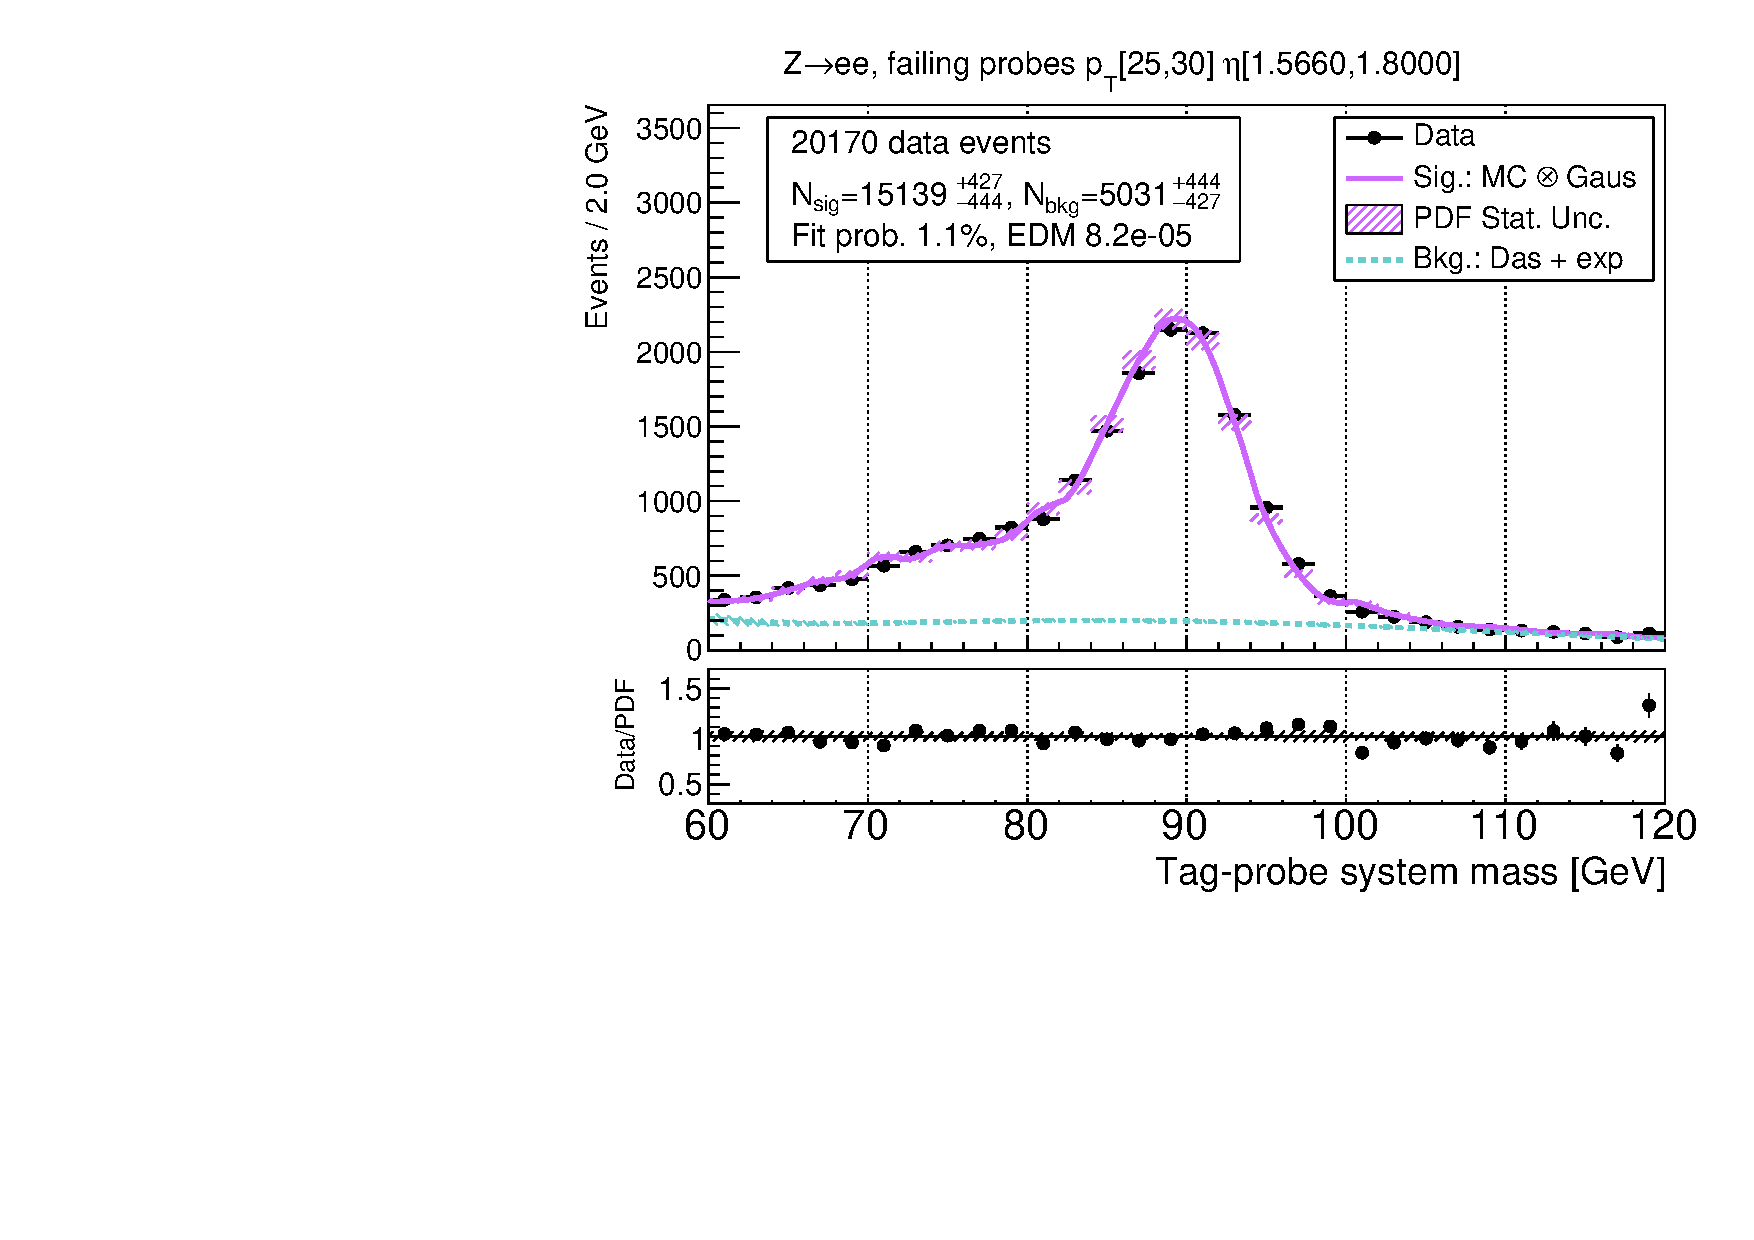
\includegraphics[width=0.49\textwidth]{figures/Zee_RecoTemplate_BkgAnalytic_fail_ptBin3_etaBin23.pdf}
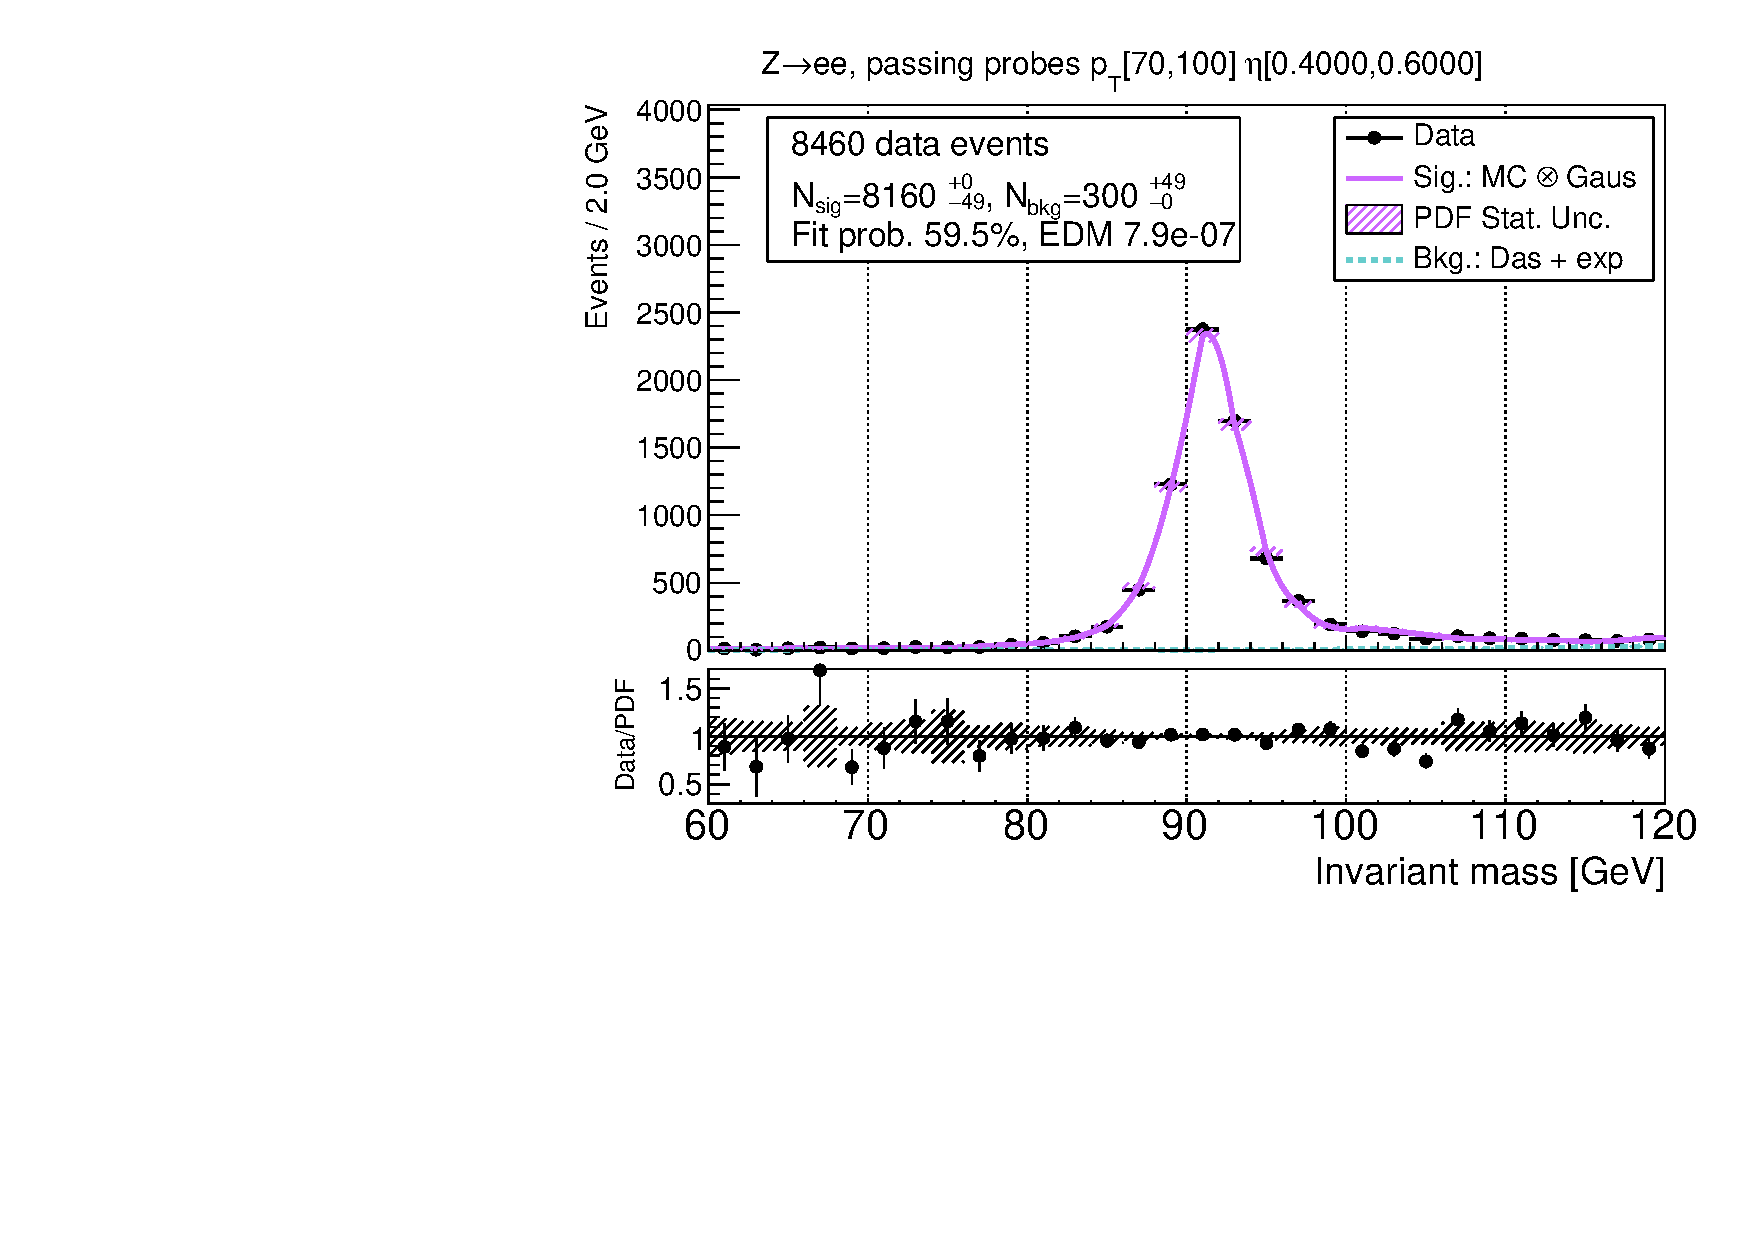
\includegraphics[width=0.49\textwidth]{figures/Zee_RecoTemplate_BkgAnalytic_pass_ptBin14_etaBin17.pdf}
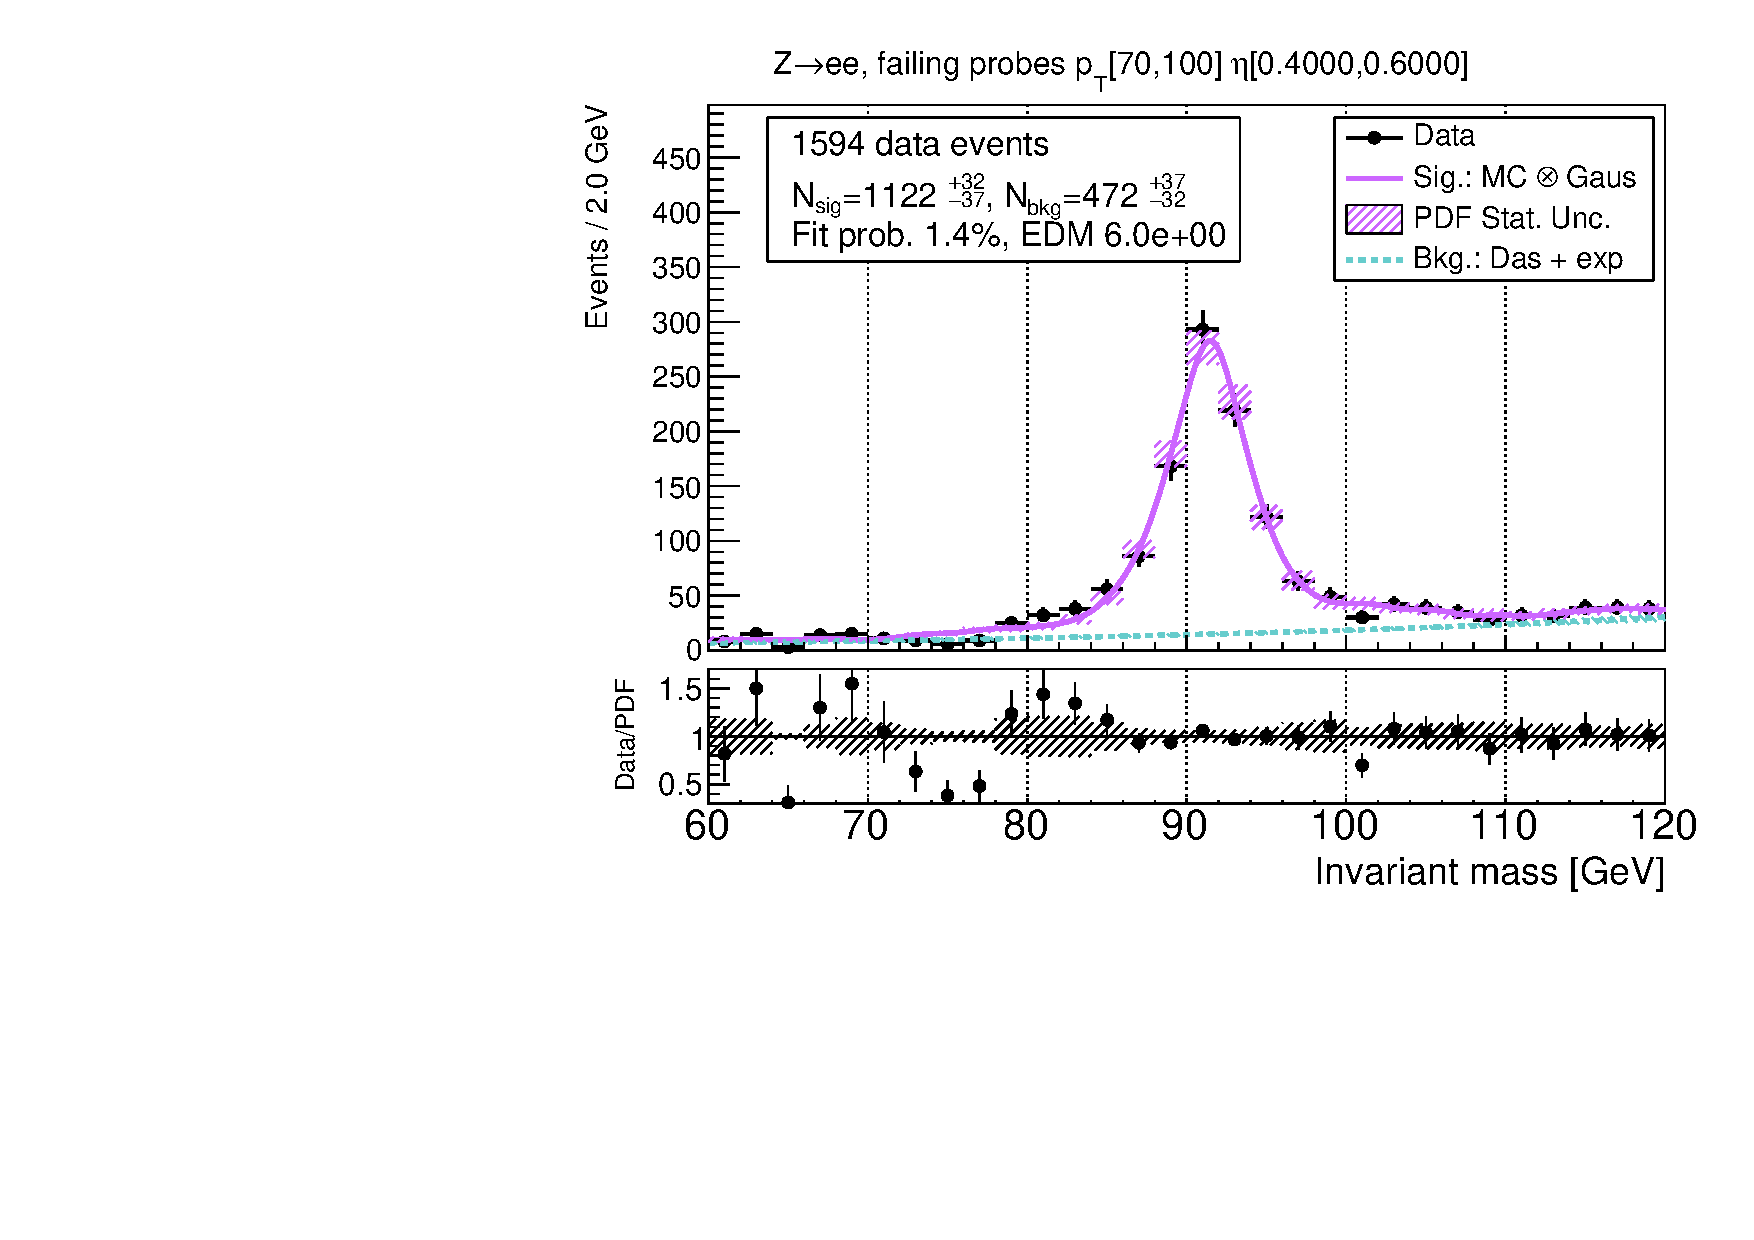
\includegraphics[width=0.49\textwidth]{figures/Zee_RecoTemplate_BkgAnalytic_fail_ptBin14_etaBin17.pdf}
\caption{Efficiency extraction fits for the Medium electron working point using the alternative analytic background shape, at higher values of electron transverse momentum.}
\label{fig:ZeeAltBkgFits2}
\end{figure}

\clearpage
\subsection{Signal resolution modeling}
We consider the uncertainty from using the simulation of the reconstructed Z resonance signal shape
by convolution with an analytic function more complex than a Gaussian to try to capture more detector resolution effects.
The difference in scale factors derived from the data efficiency extraction fits using the two methods
is taken as the systematic uncertainty due to signal resolution modeling.
The alternative function is a single Gaussian with asymmetric, exponential tails.

Examples of fits for 2016 run eras B to F with the alternative resolution function are shown for dimuons in
Figures ~\ref{fig:ZmmAltSigResFits1} and~\ref{fig:ZmmAltSigResFits2}, 
and for dielectrons in Figures~\ref{fig:ZeeAltSigResFits1} and~\ref{fig:ZeeAltSigResFits2}.
These may be compared with the fits using the nominal resolution function
in section \ref{sec:tnpfits}.
The difference in the Data/MC scale factors derived using the two methods is taken as a systematic; 
see Figures~\ref{fig:ZmmSystSigRes} and~\ref{fig:ZeeSystSigRes}.

\begin{figure}
\centering
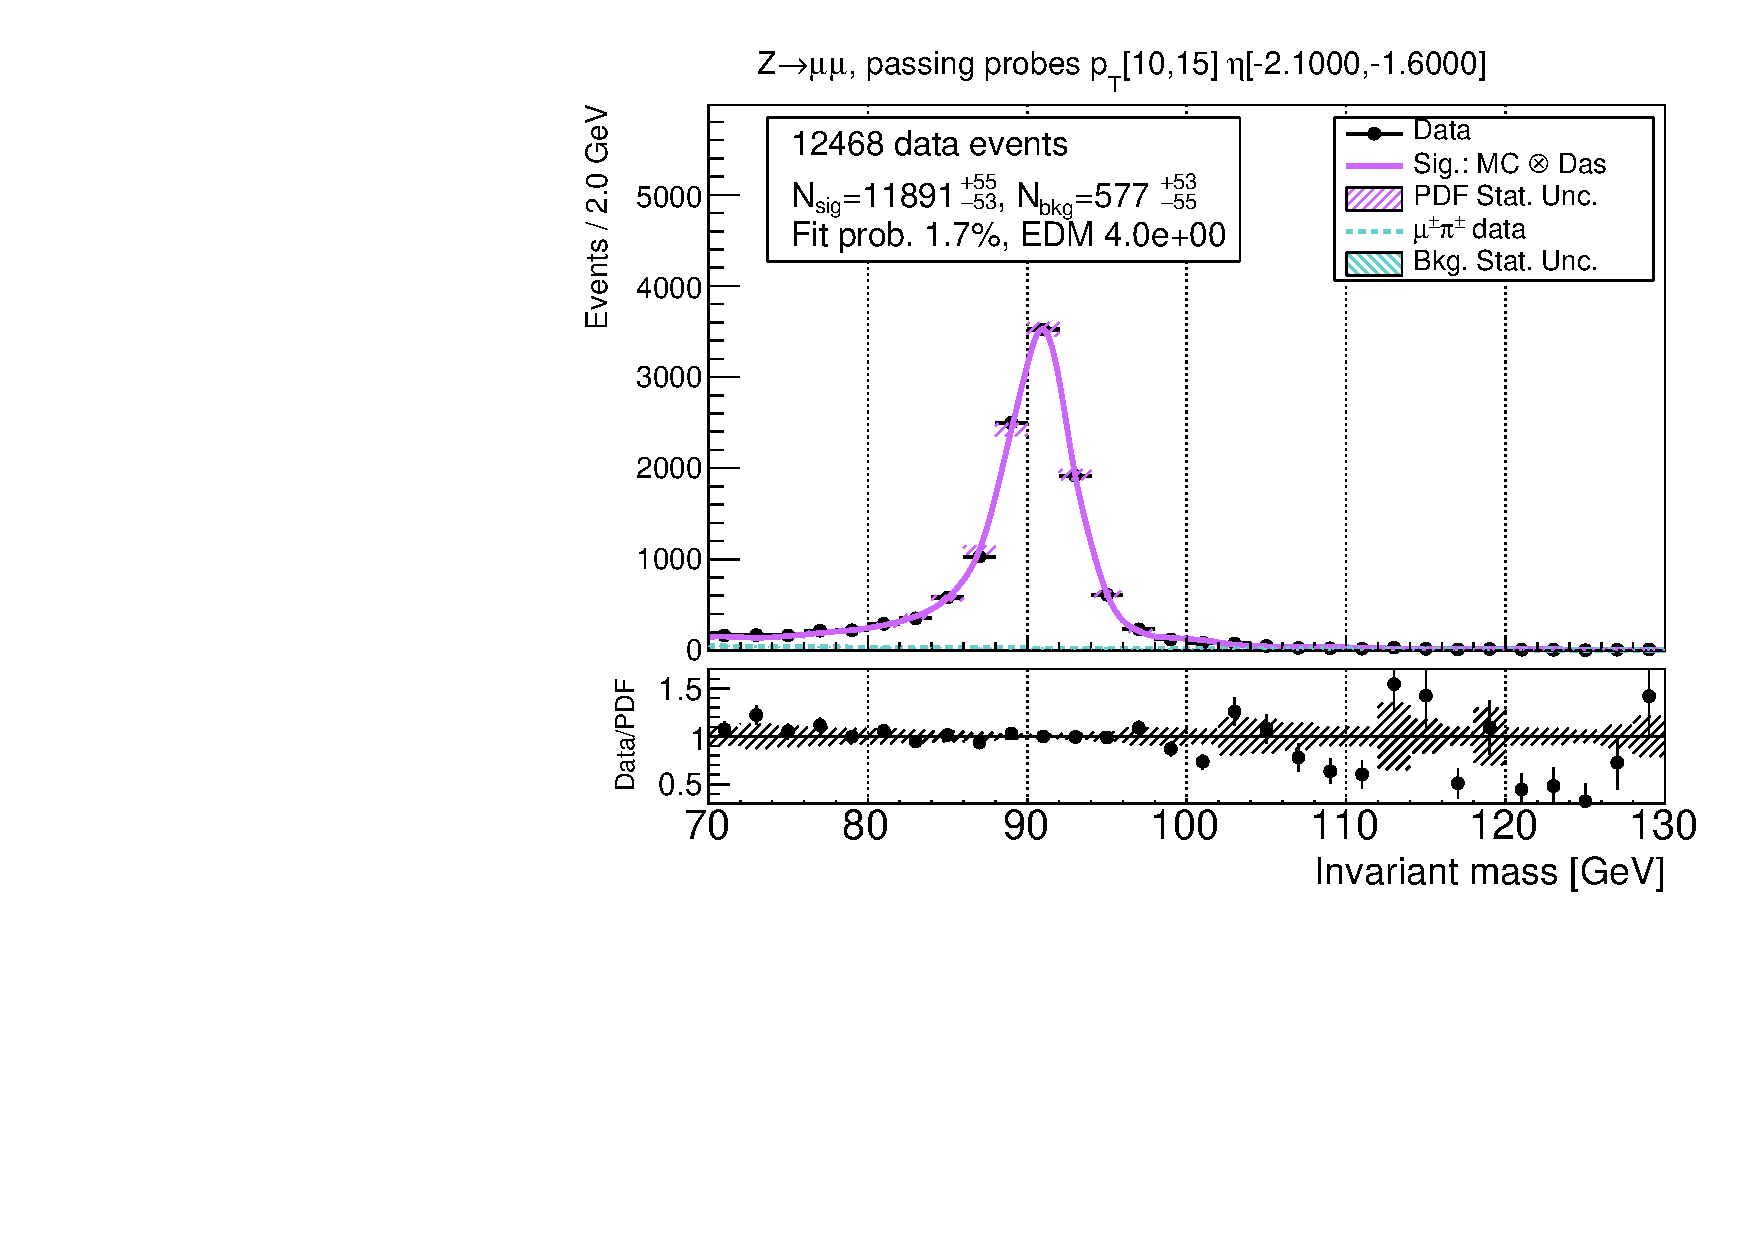
\includegraphics[width=0.49\textwidth]{figures/Zmm_ResFunc_BkgLPi_pass_ptBin0_etaBin1.pdf}
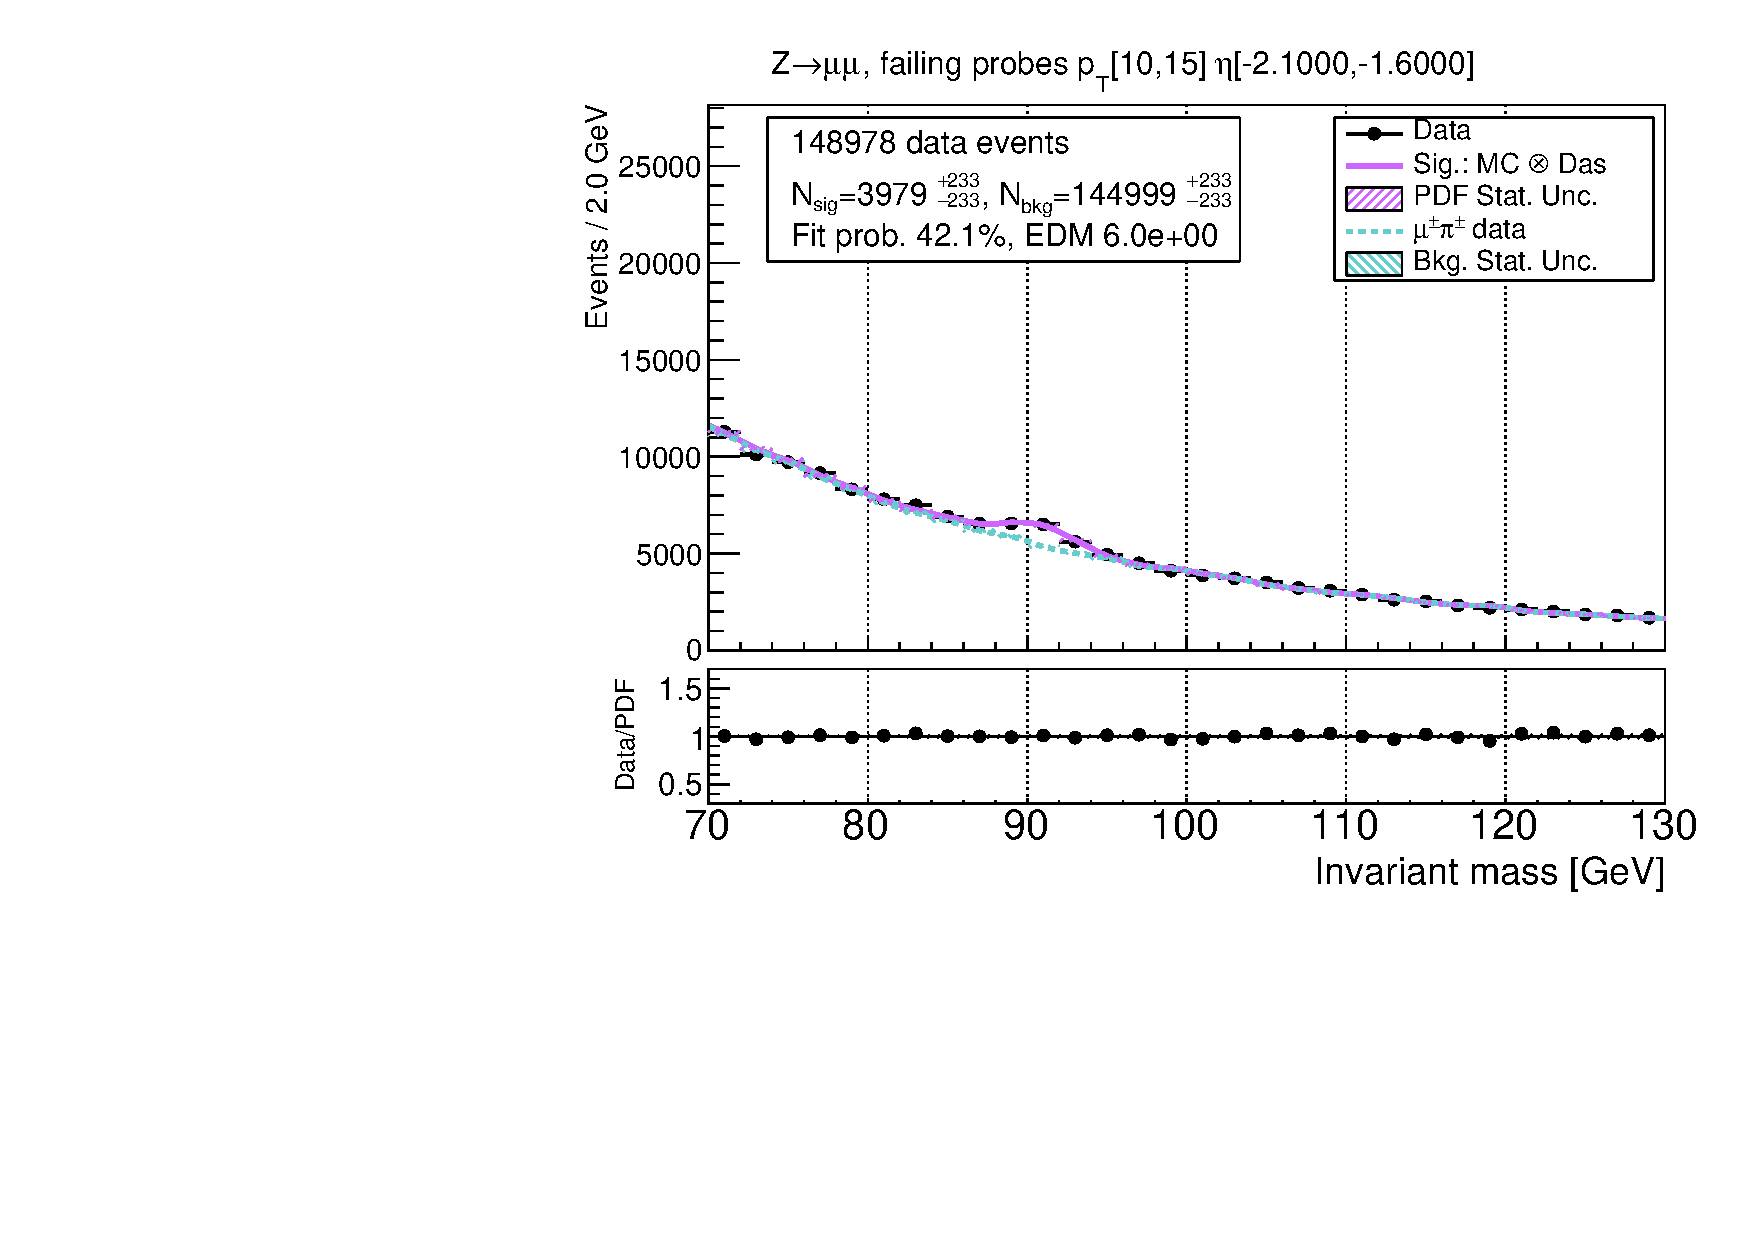
\includegraphics[width=0.49\textwidth]{figures/Zmm_ResFunc_BkgLPi_fail_ptBin0_etaBin1.pdf}
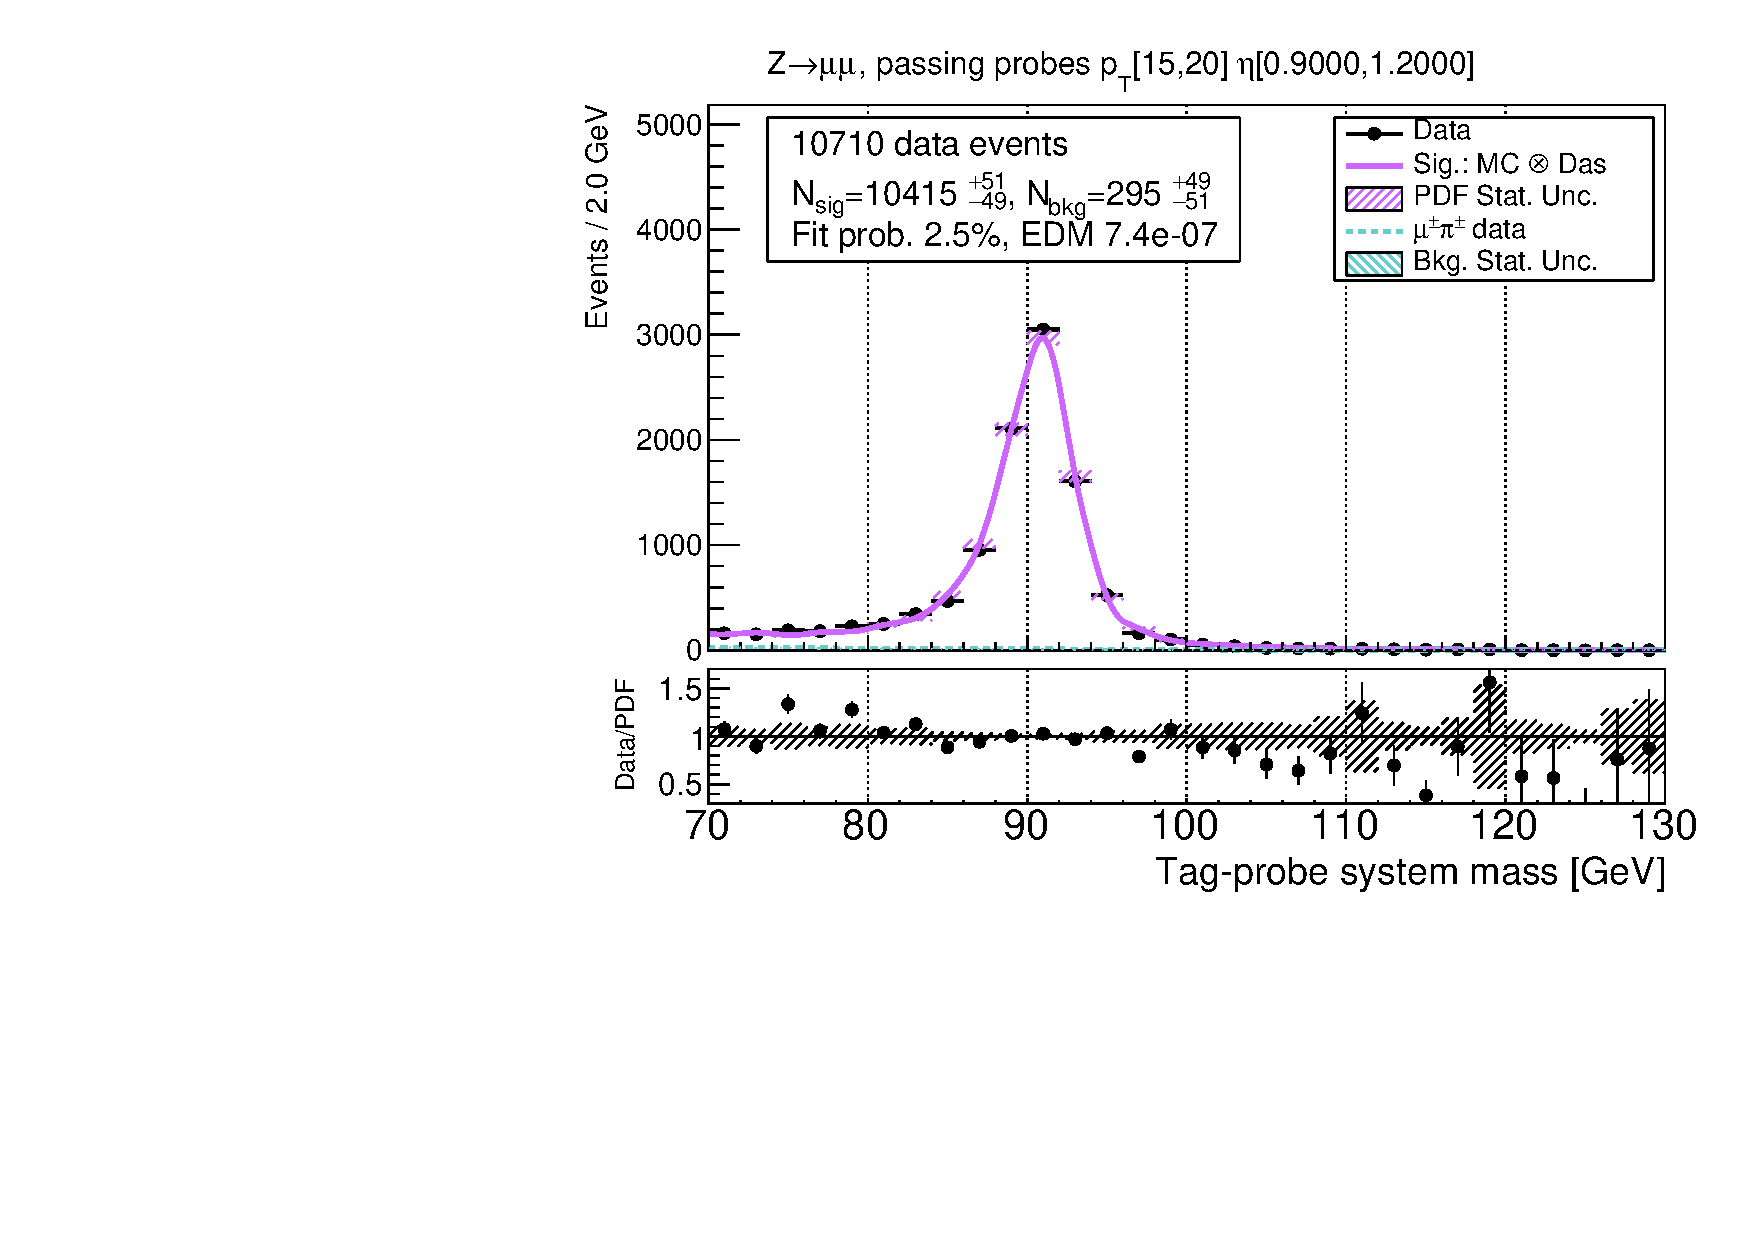
\includegraphics[width=0.49\textwidth]{figures/Zmm_ResFunc_BkgLPi_pass_ptBin1_etaBin9.pdf}
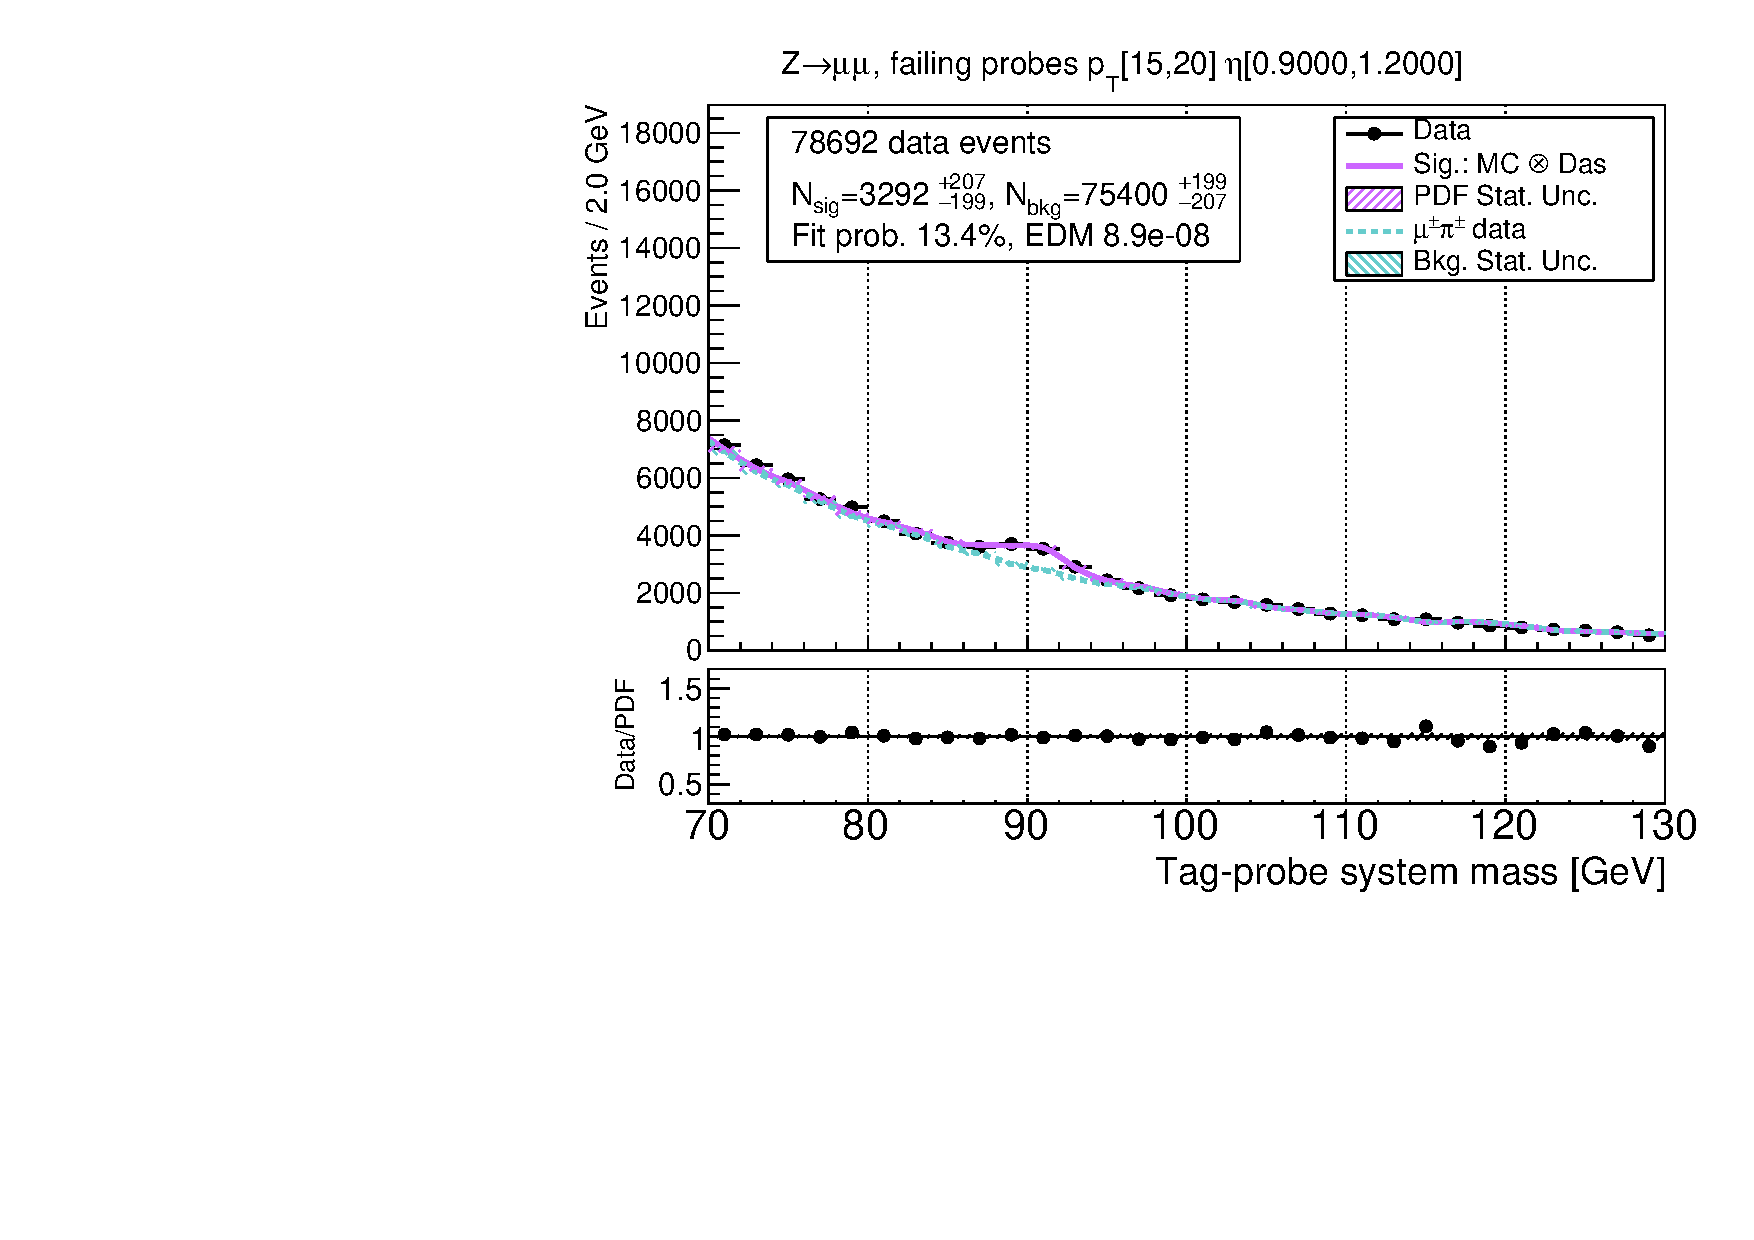
\includegraphics[width=0.49\textwidth]{figures/Zmm_ResFunc_BkgLPi_fail_ptBin1_etaBin9.pdf}
\caption{Efficiency extraction fits for the Medium muon working point using the analytic detector resolution function, at low muon transverse momentum.}
\label{fig:ZmmAltSigResFits1}
\end{figure}

\begin{figure}
\centering
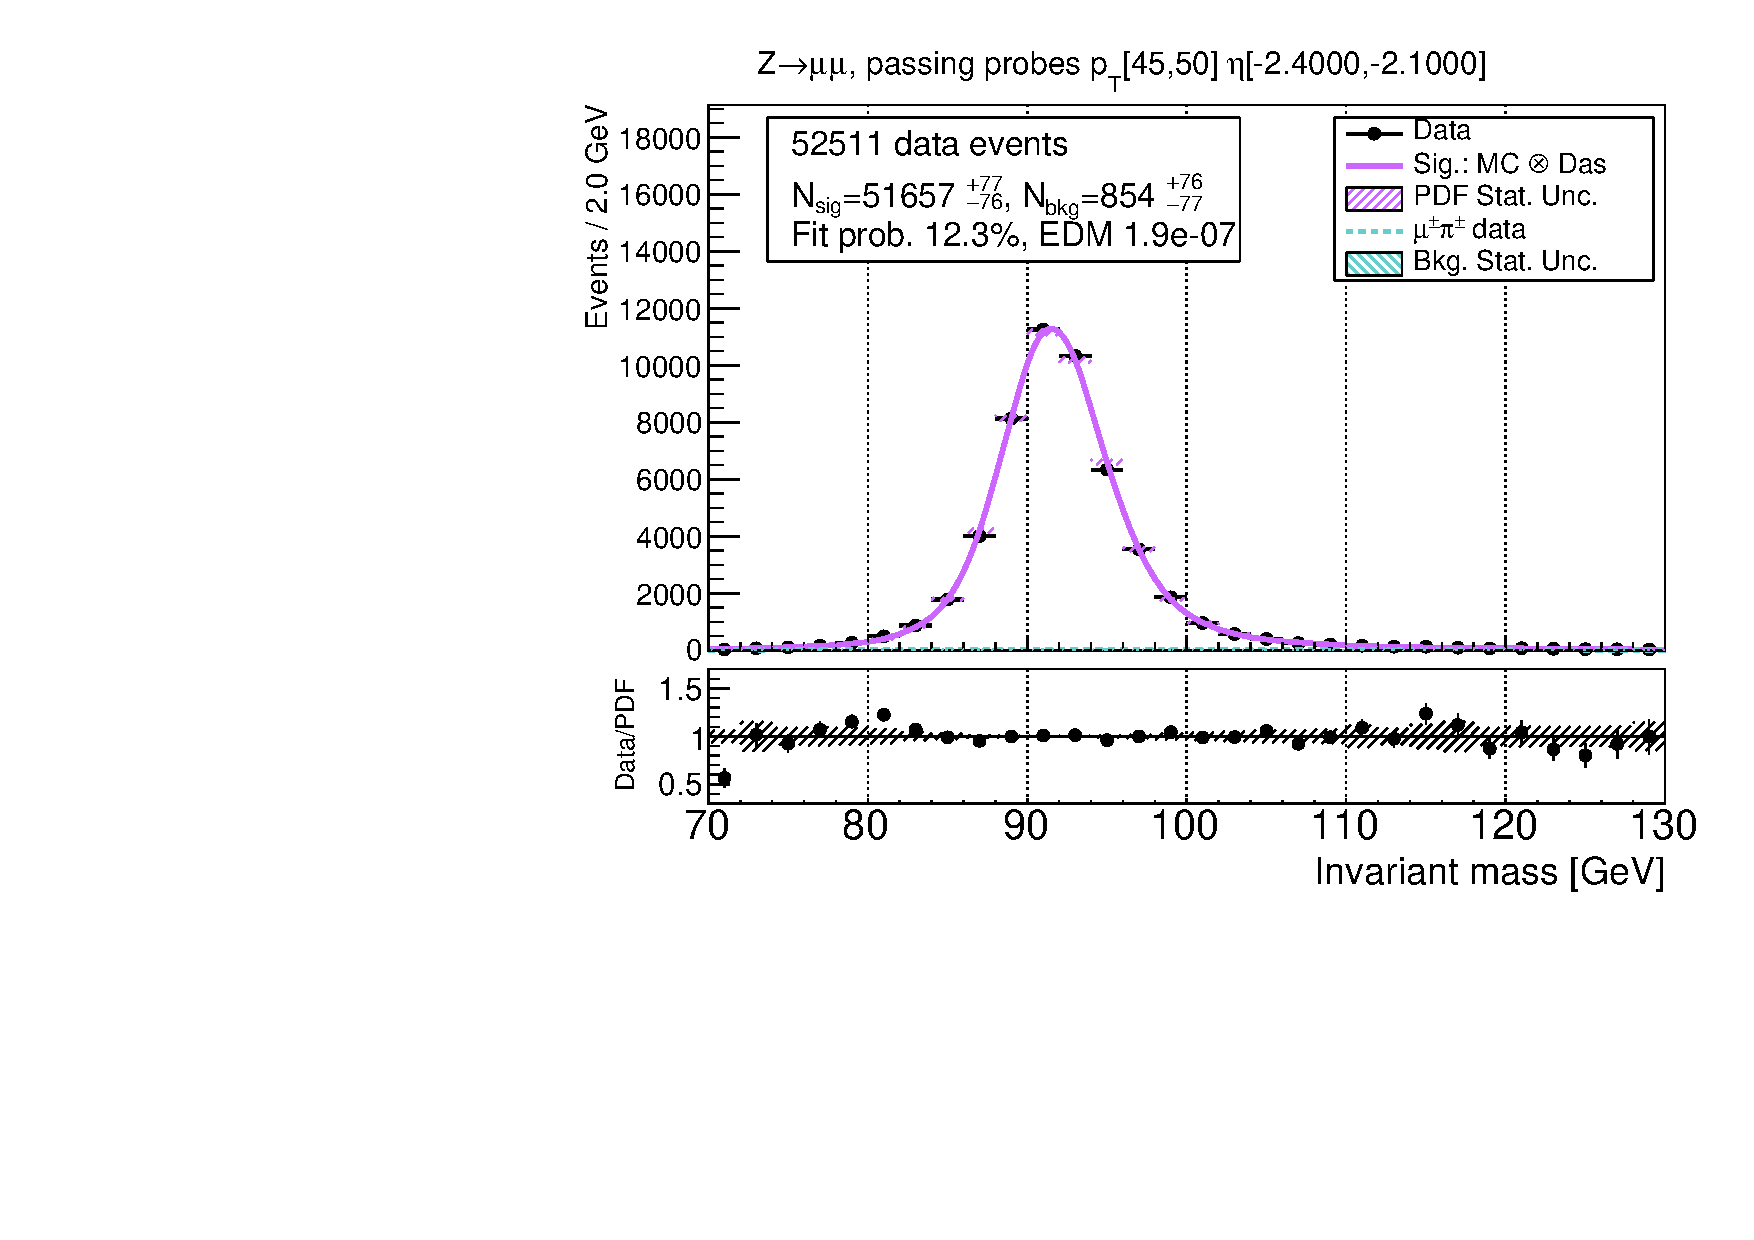
\includegraphics[width=0.49\textwidth]{figures/Zmm_ResFunc_BkgLPi_pass_ptBin7_etaBin0.pdf}
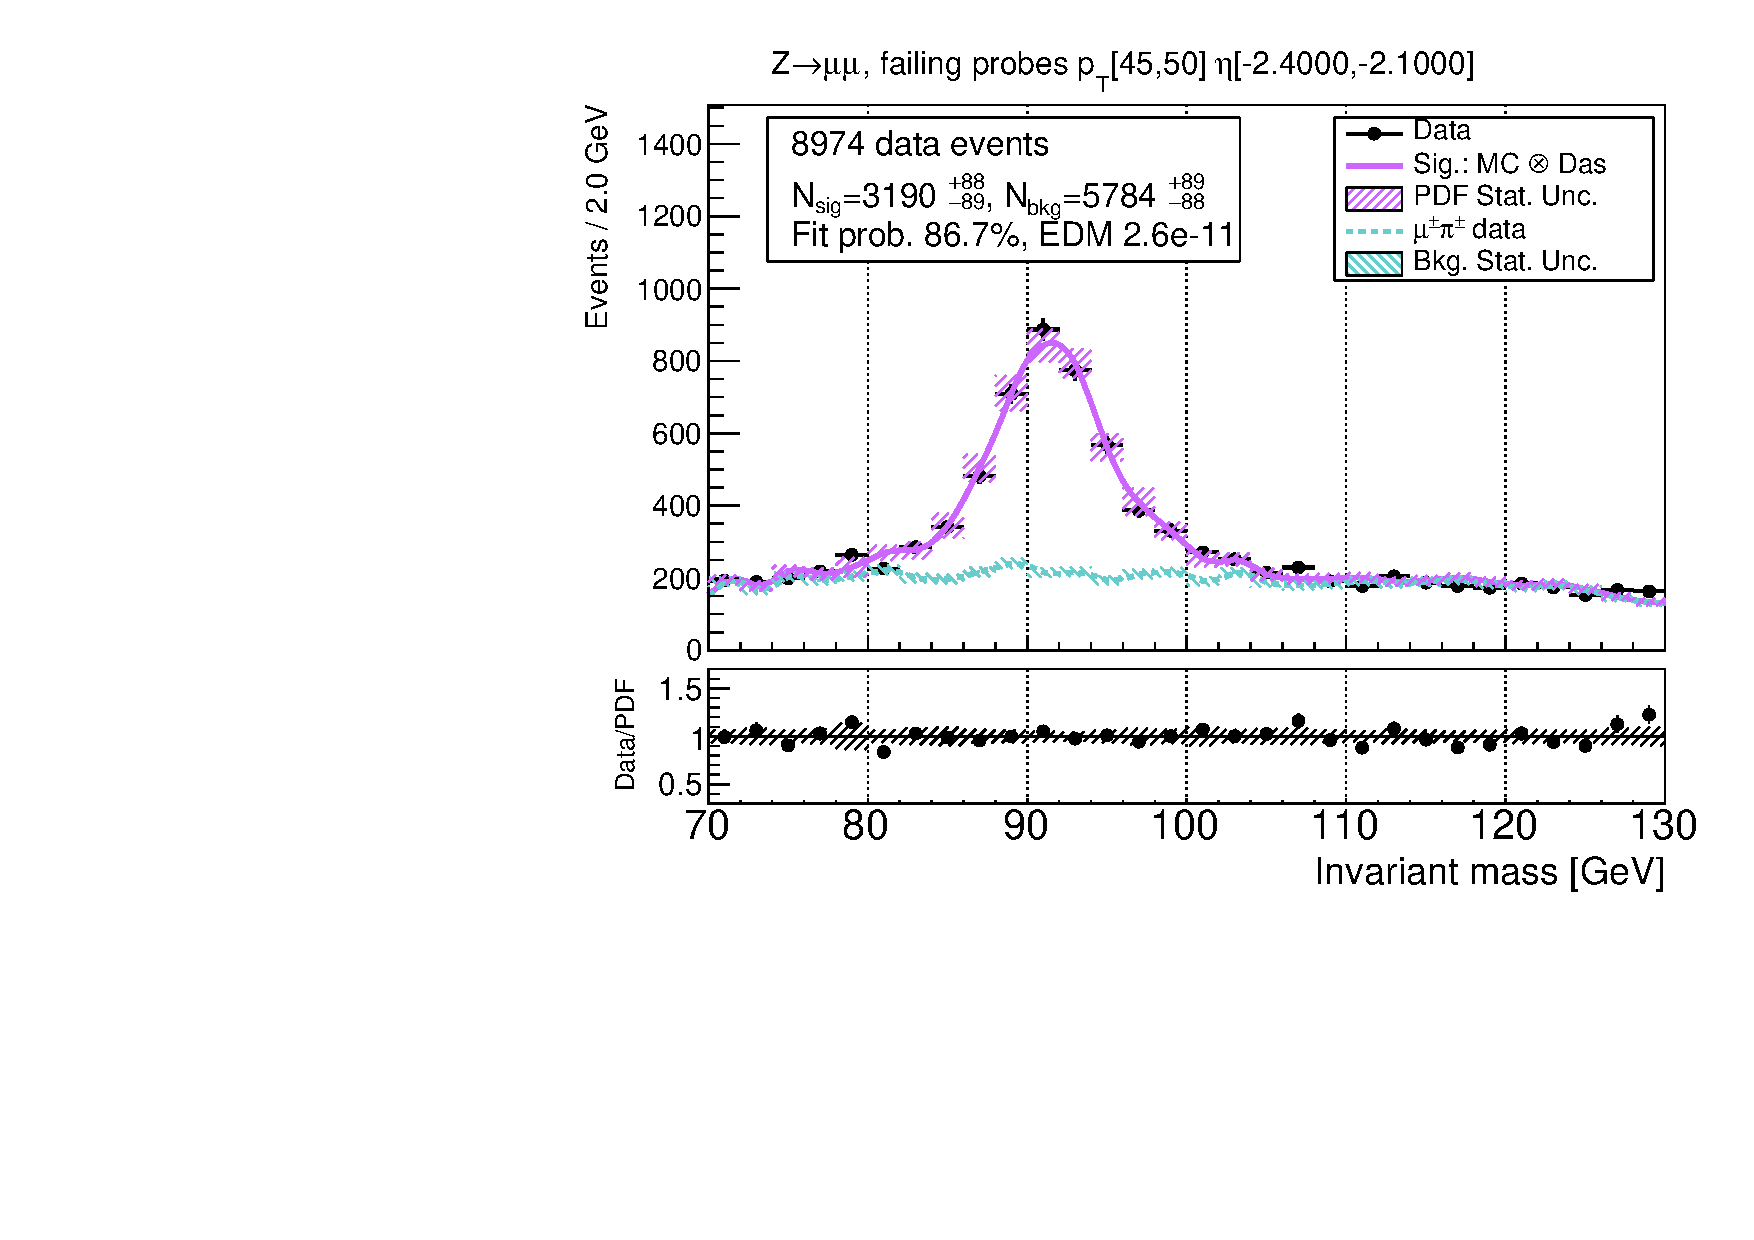
\includegraphics[width=0.49\textwidth]{figures/Zmm_ResFunc_BkgLPi_fail_ptBin7_etaBin0.pdf}
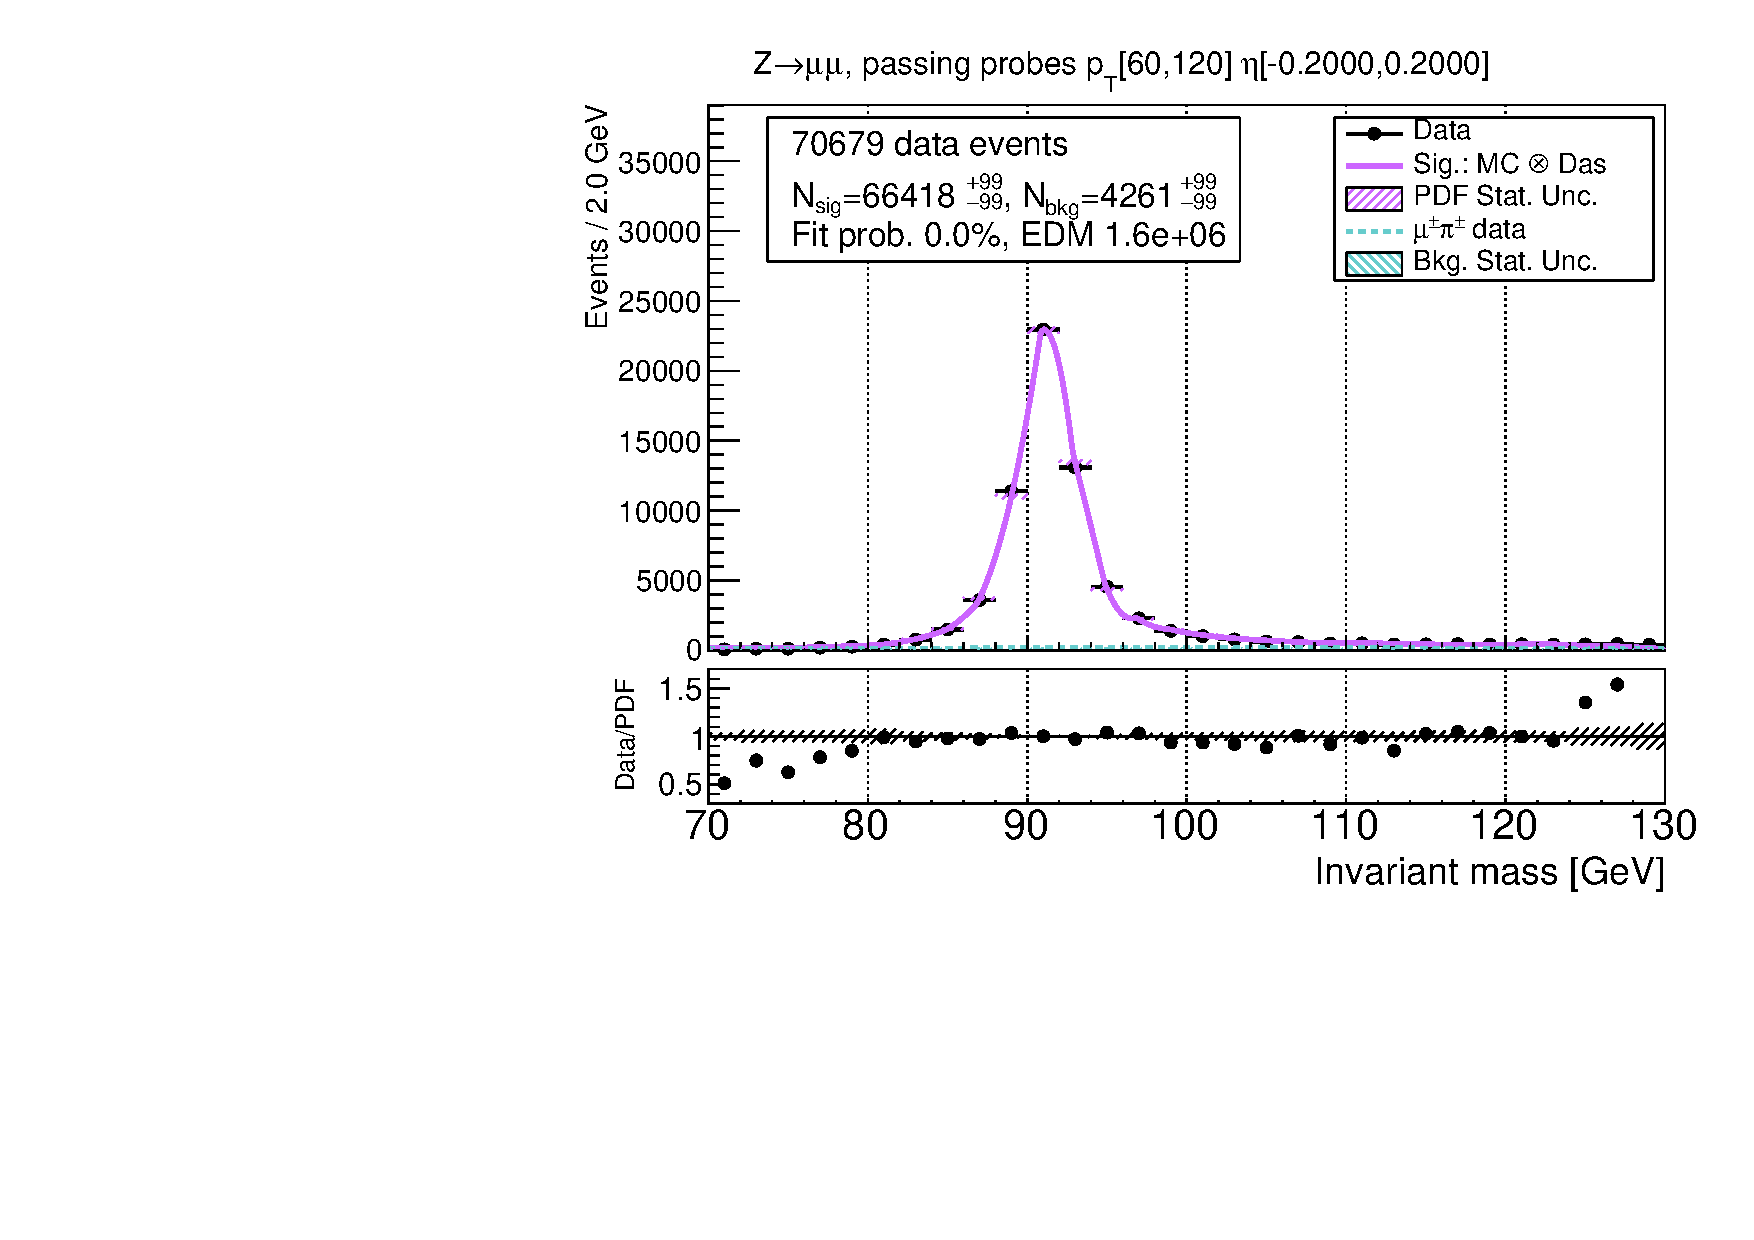
\includegraphics[width=0.49\textwidth]{figures/Zmm_ResFunc_BkgLPi_pass_ptBin10_etaBin6.pdf}
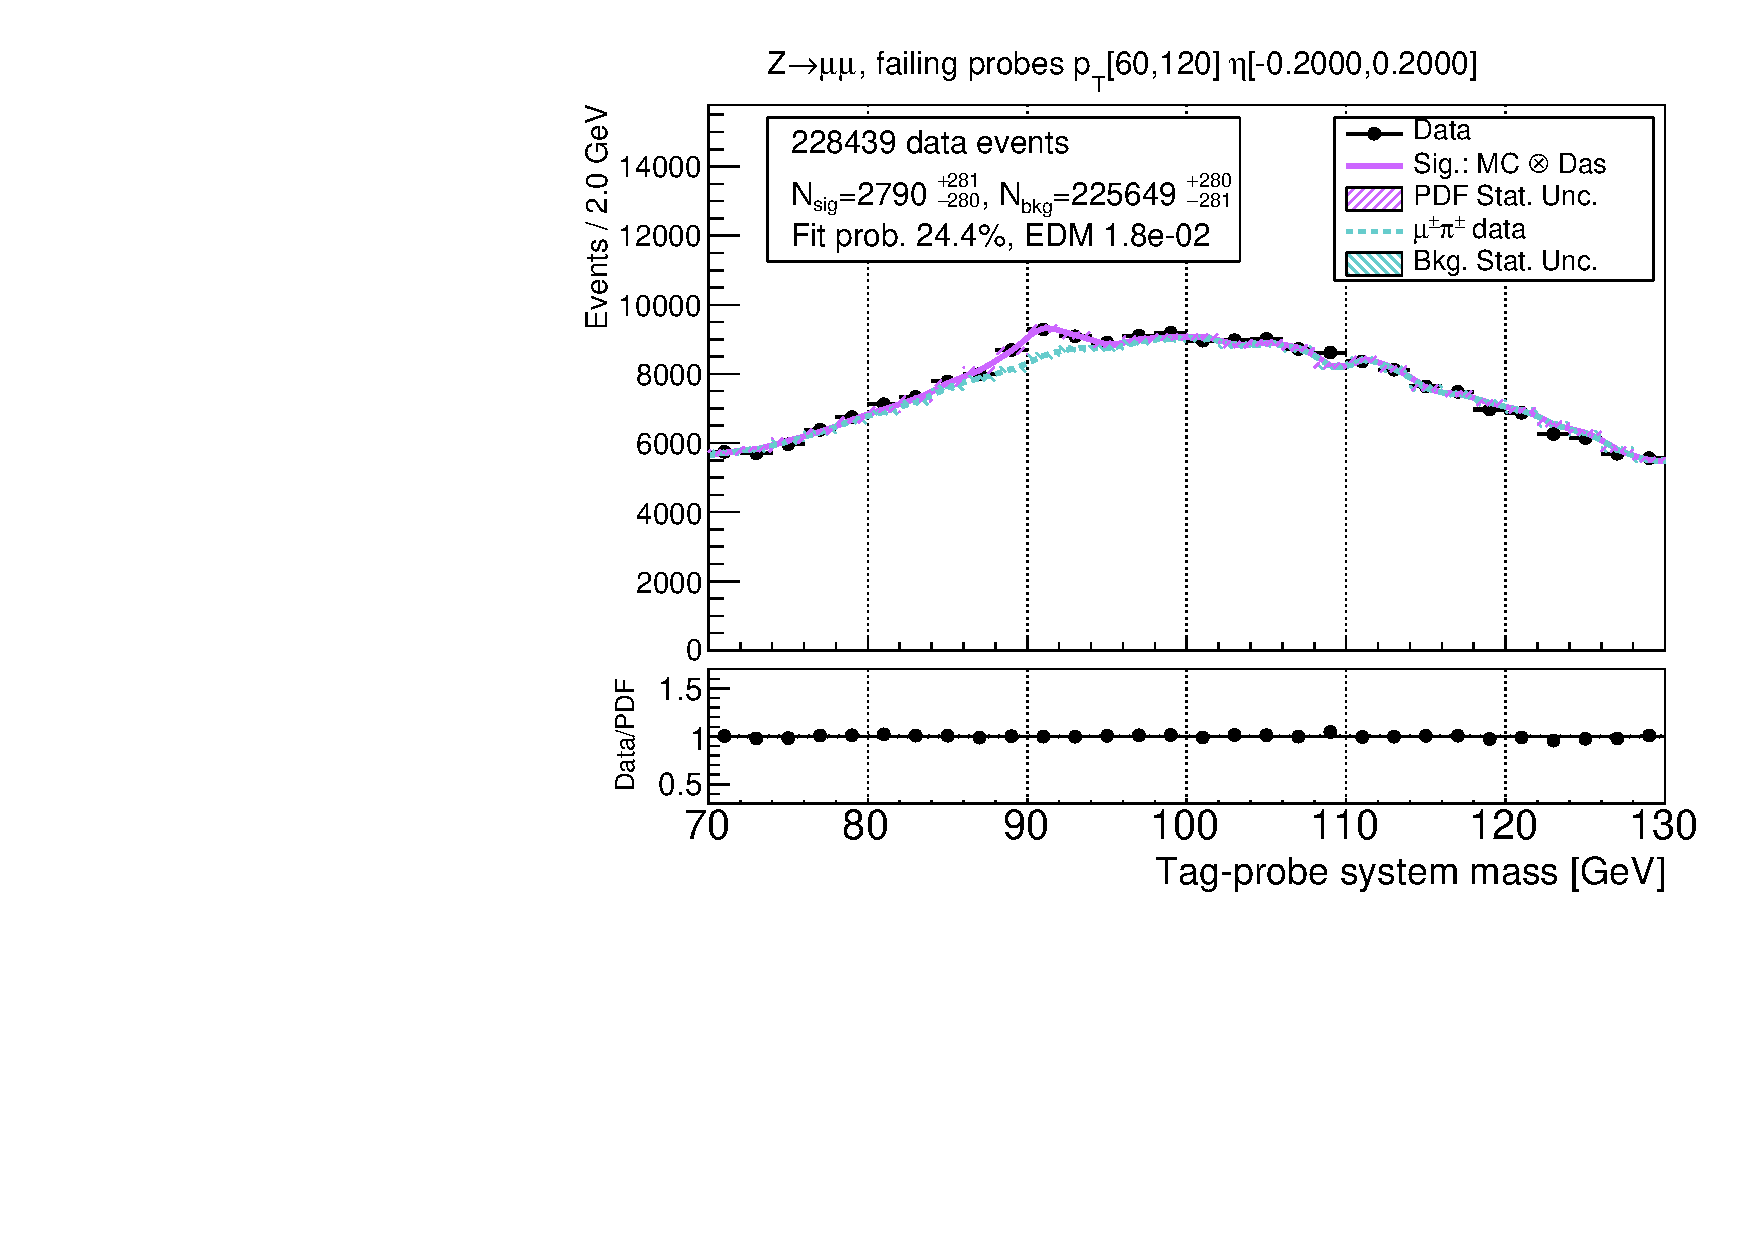
\includegraphics[width=0.49\textwidth]{figures/Zmm_ResFunc_BkgLPi_fail_ptBin10_etaBin6.pdf}
\caption{Efficiency extraction fits for the Medium muon working point using the analytic detector resolution function, at higher values of muon transverse momentum.}
\label{fig:ZmmAltSigResFits2}
\end{figure}

\begin{figure}
\centering
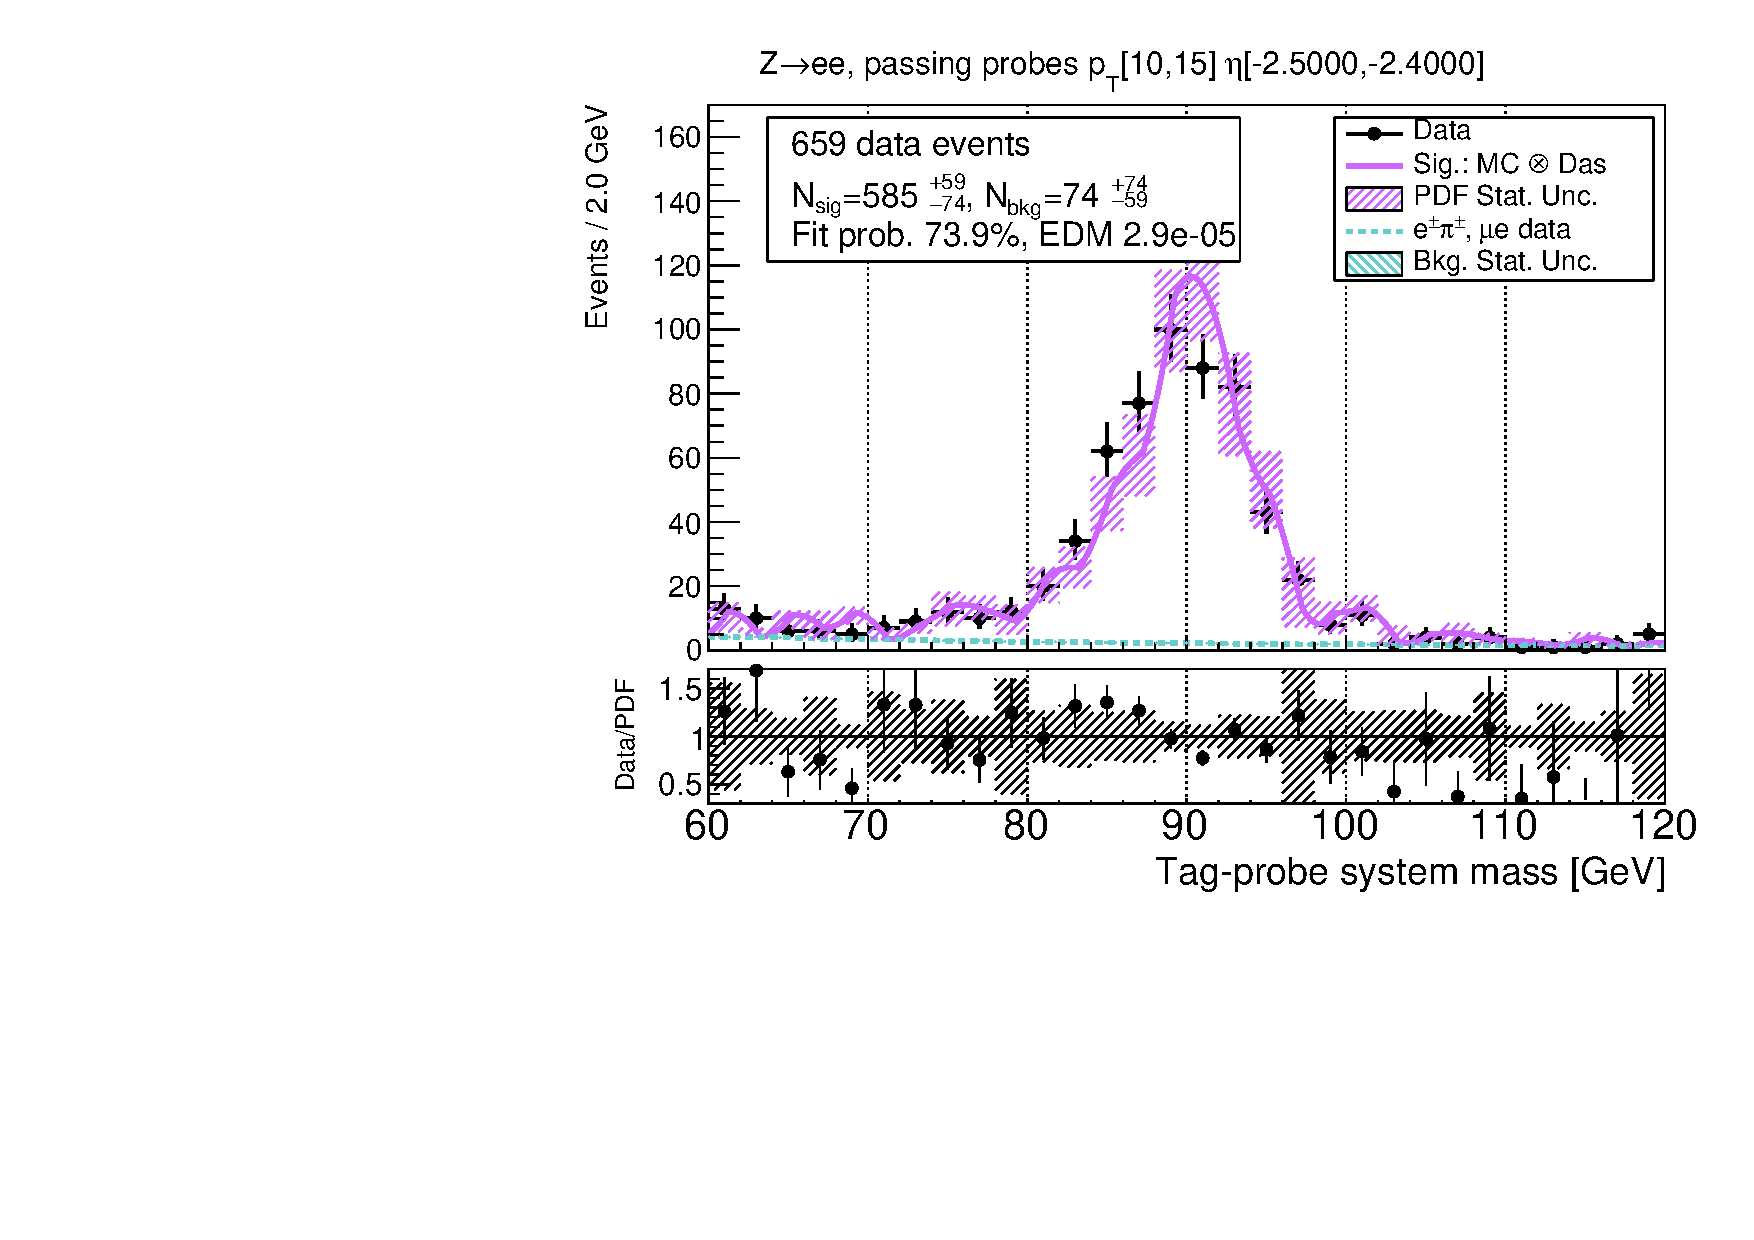
\includegraphics[width=0.49\textwidth]{figures/Zee_ResFunc_BkgLPiEMu_pass_ptBin0_etaBin0.pdf}
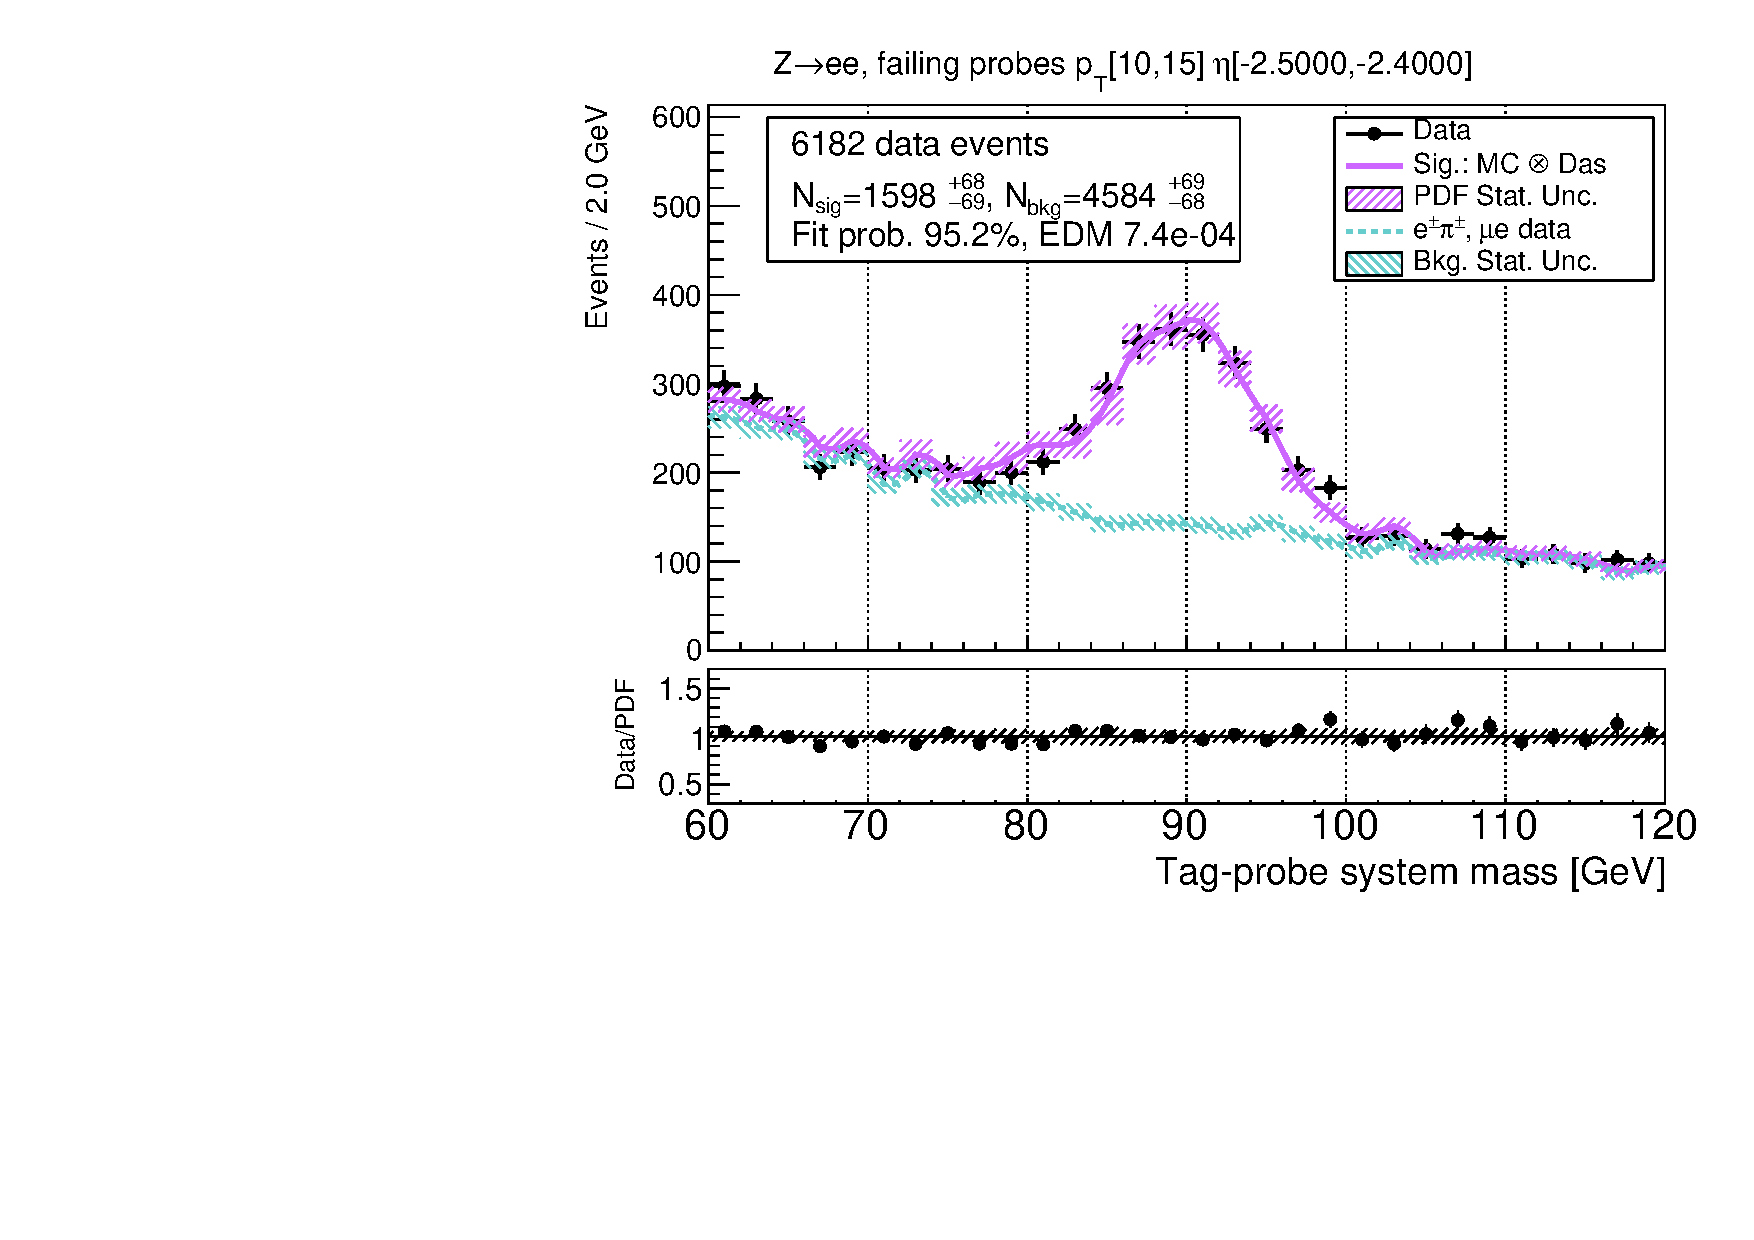
\includegraphics[width=0.49\textwidth]{figures/Zee_ResFunc_BkgLPiEMu_fail_ptBin0_etaBin0.pdf}
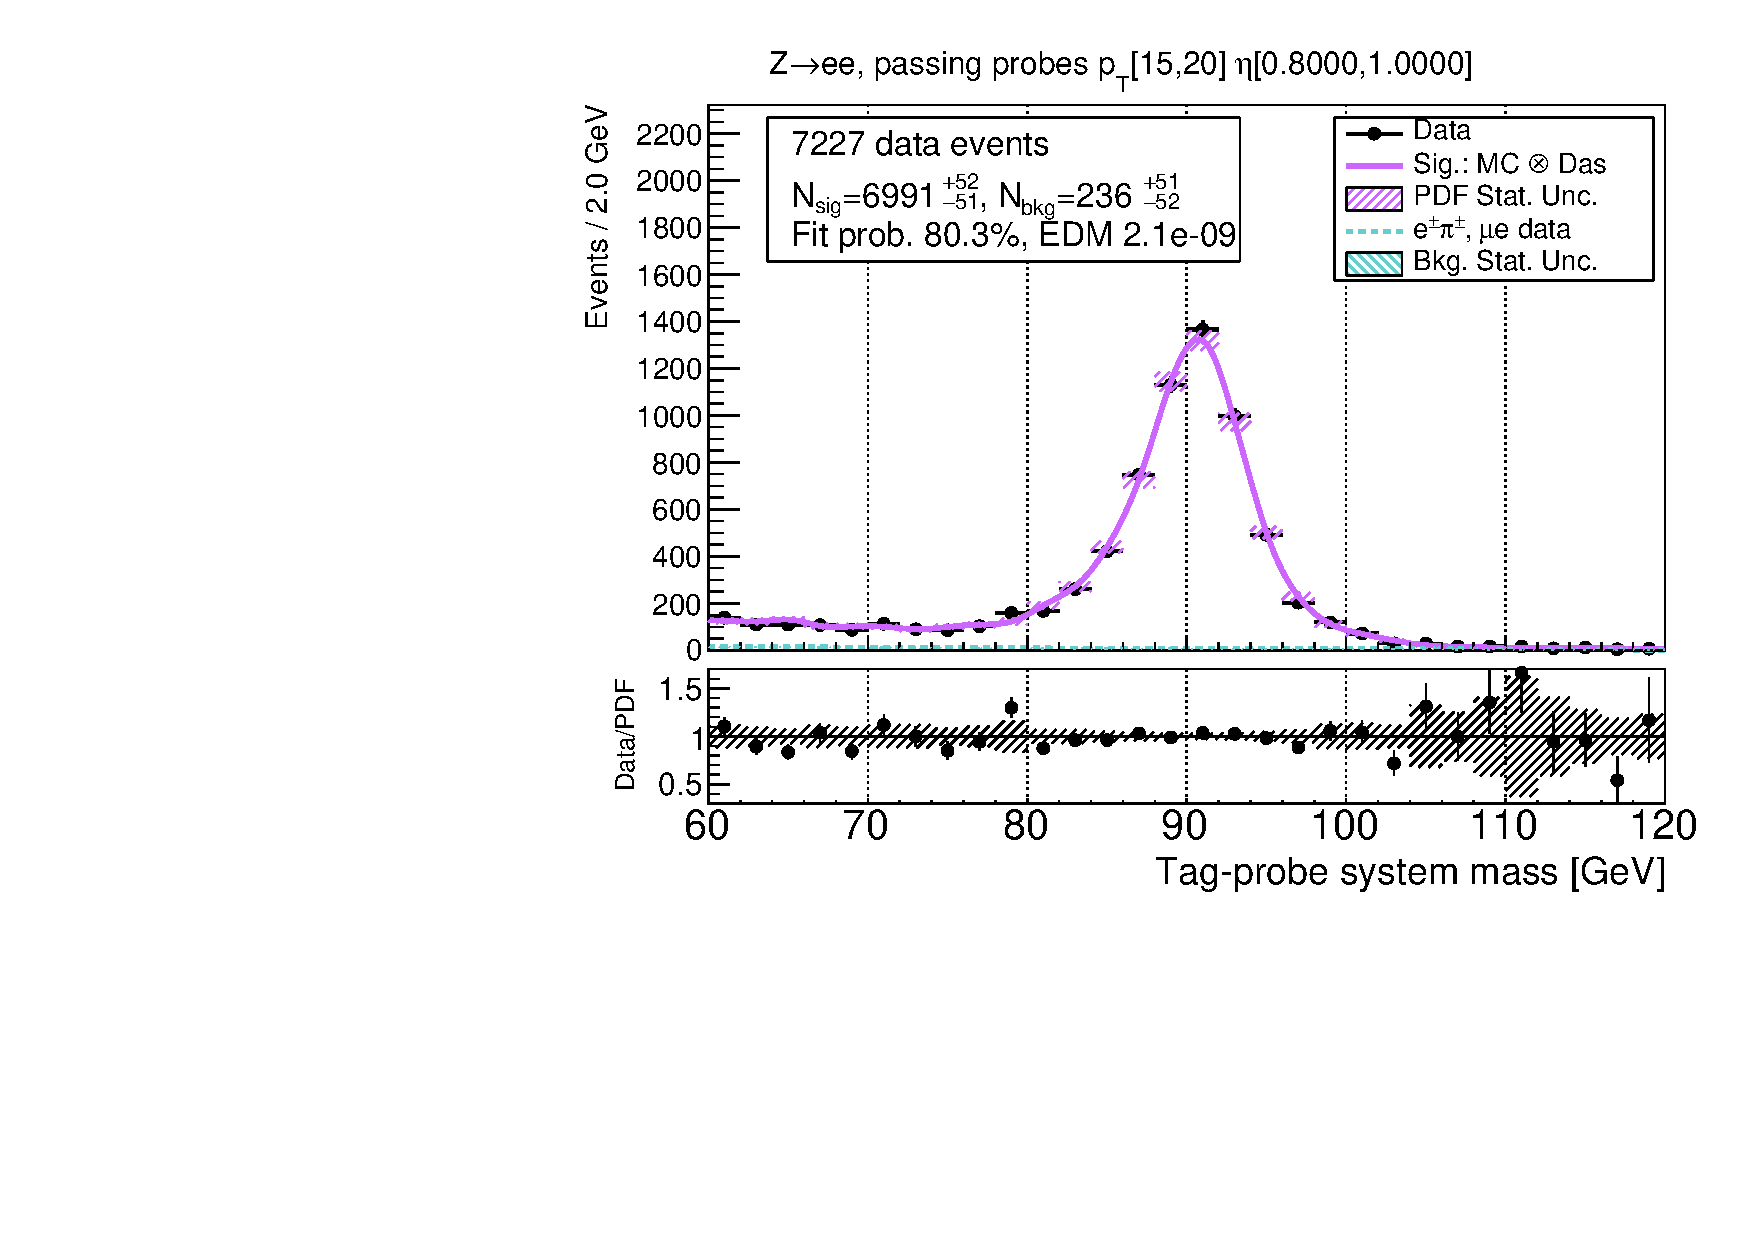
\includegraphics[width=0.49\textwidth]{figures/Zee_ResFunc_BkgLPiEMu_pass_ptBin1_etaBin19.pdf}
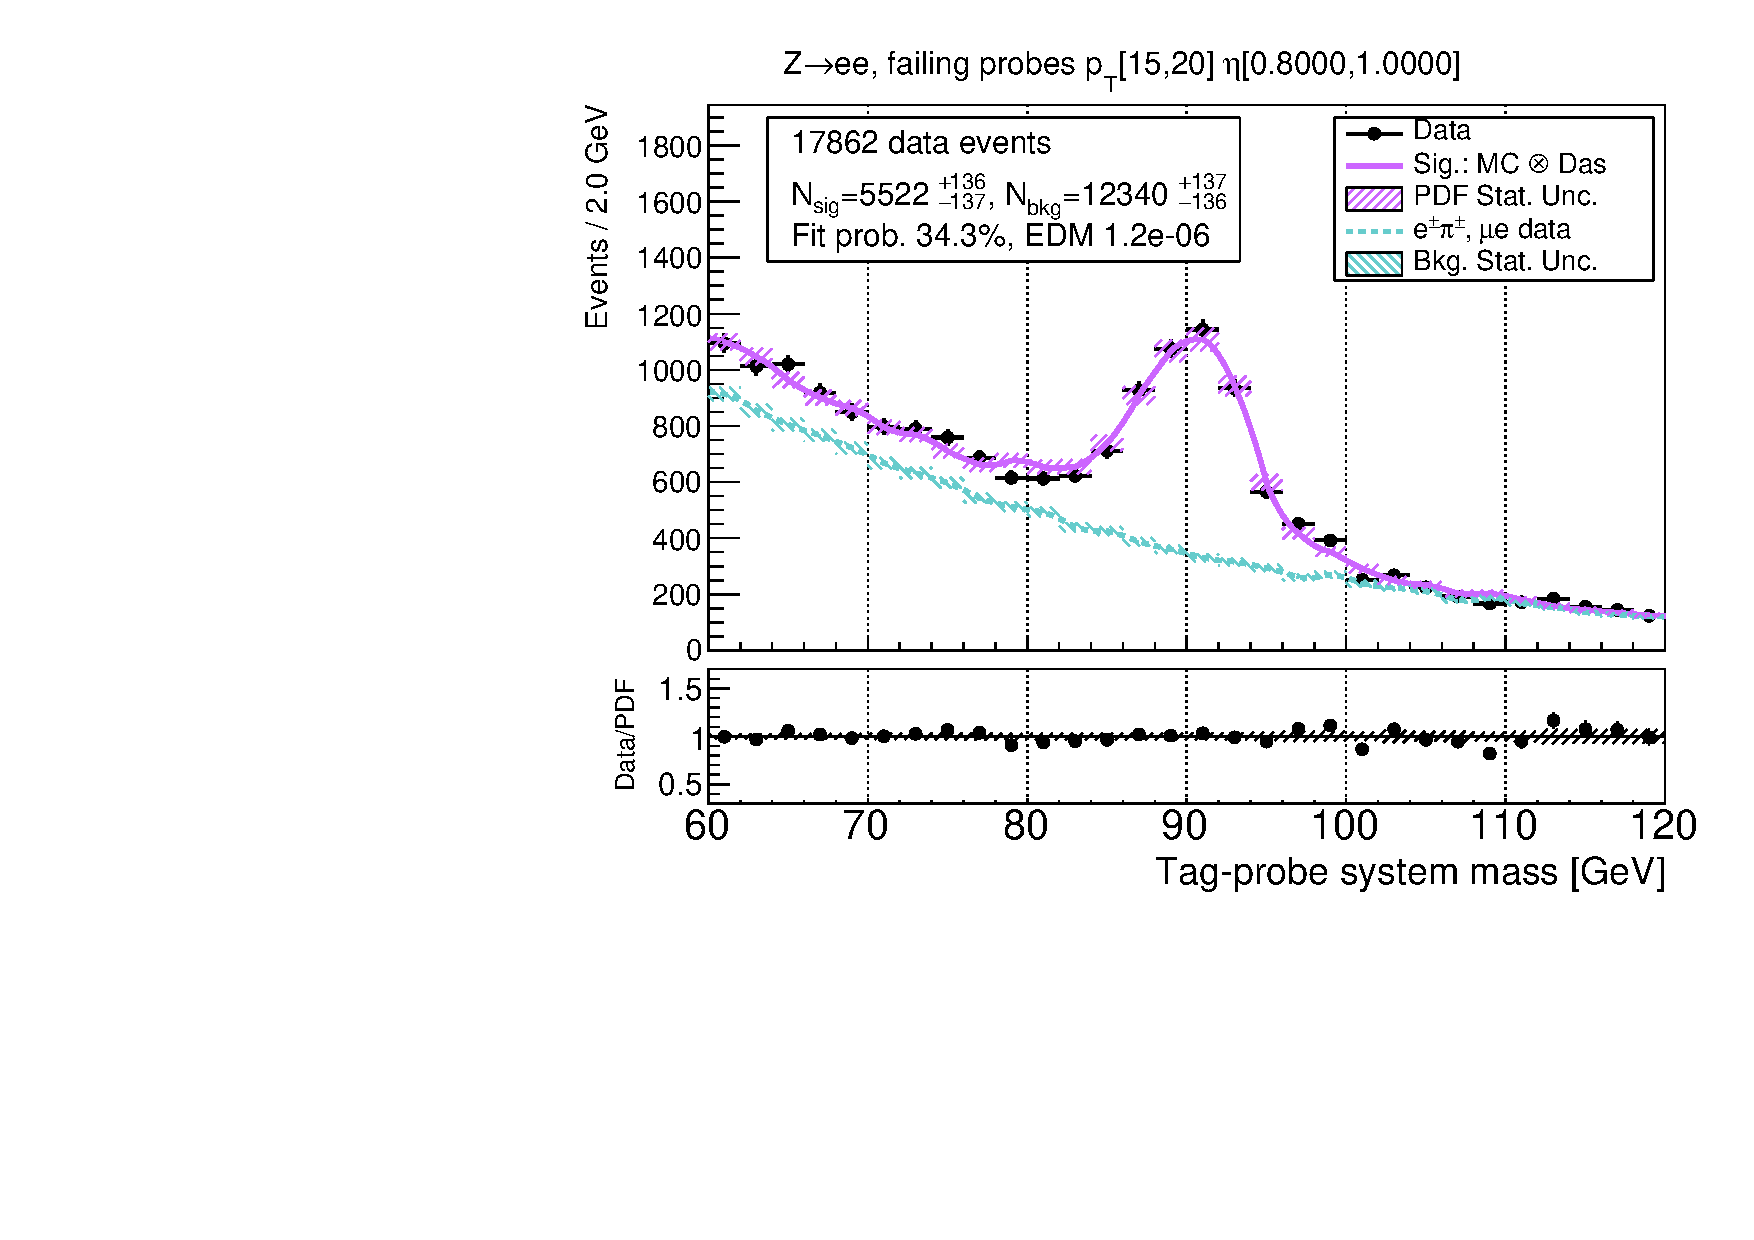
\includegraphics[width=0.49\textwidth]{figures/Zee_ResFunc_BkgLPiEMu_fail_ptBin1_etaBin19.pdf}
\caption{Efficiency extraction fits for the Medium electron working point using the analytic detector resolution function, at low electron transverse momentum.}
\label{fig:ZeeAltSigResFits1}
\end{figure}

\begin{figure}
\centering
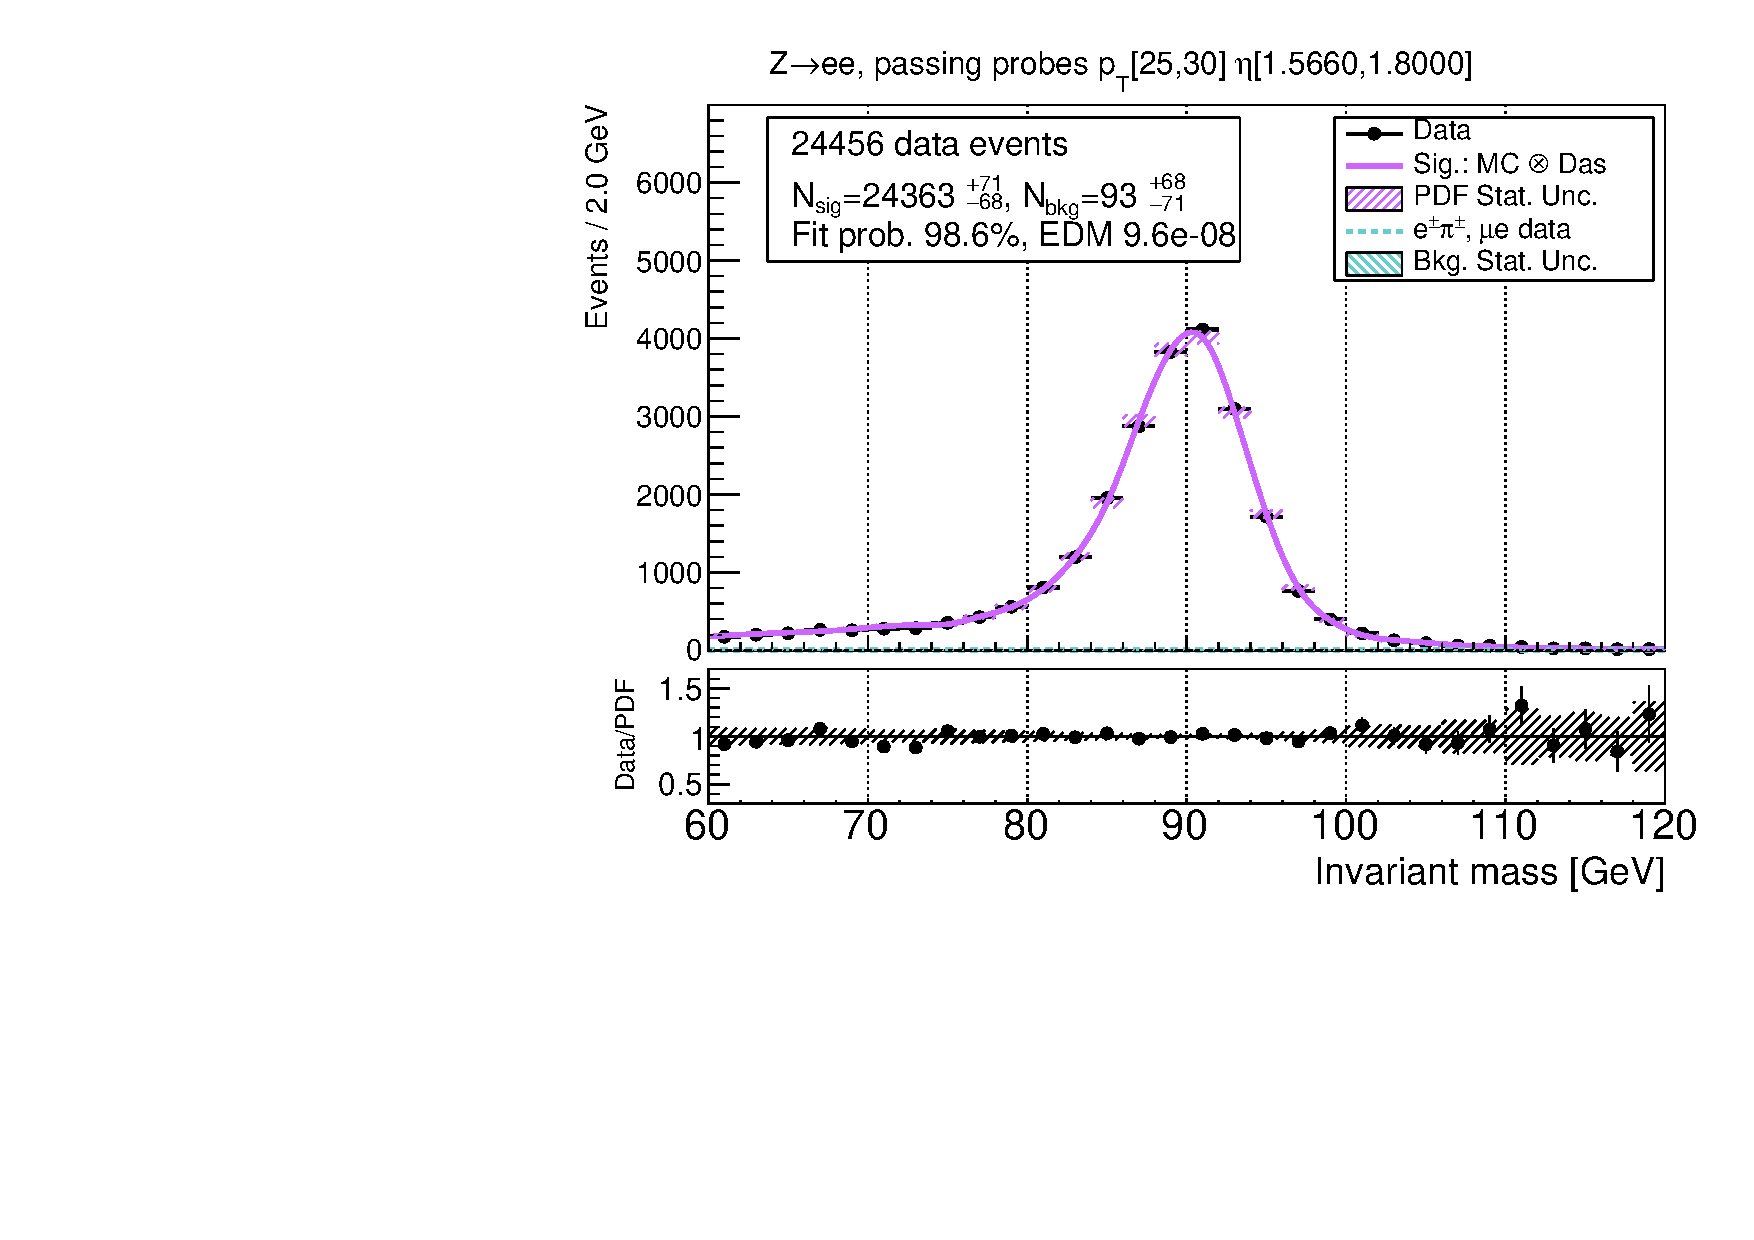
\includegraphics[width=0.49\textwidth]{figures/Zee_ResFunc_BkgLPiEMu_pass_ptBin3_etaBin23.pdf}
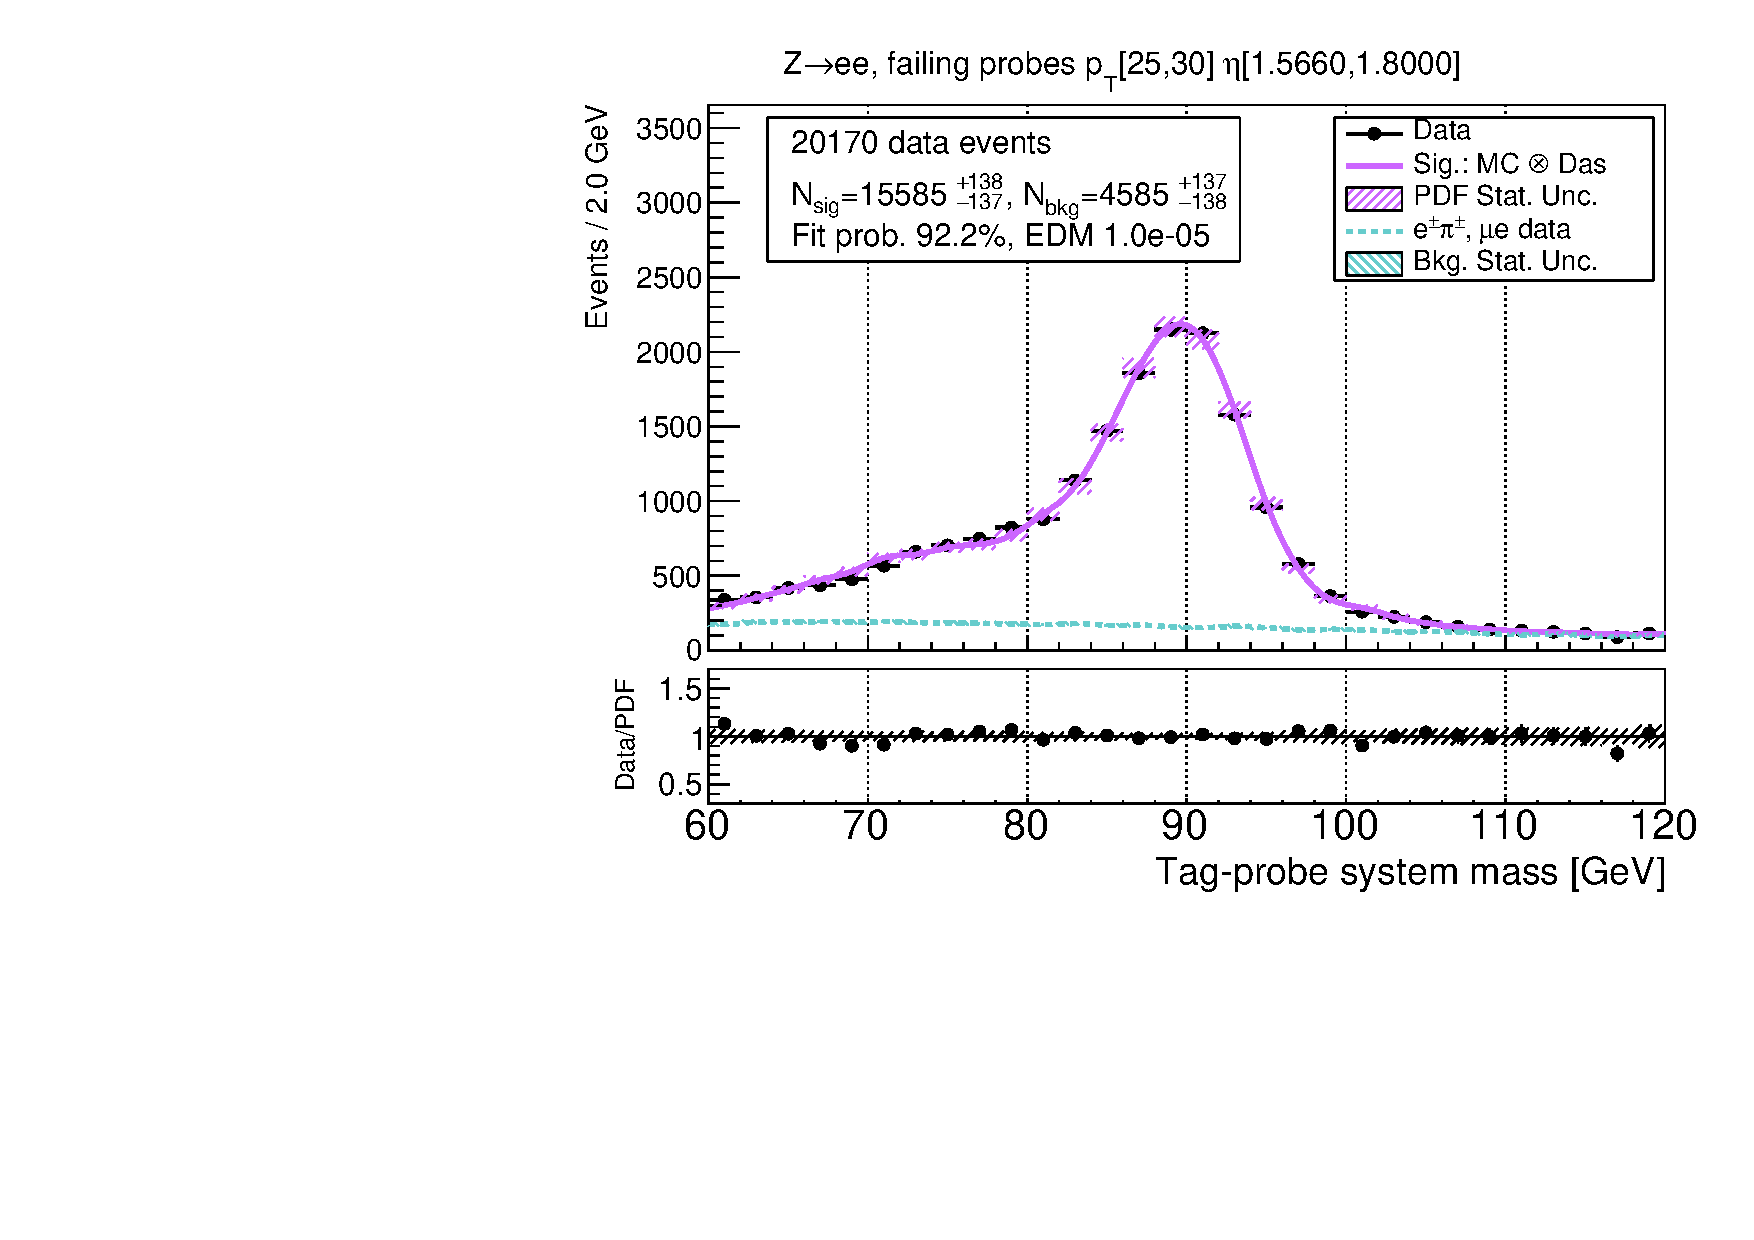
\includegraphics[width=0.49\textwidth]{figures/Zee_ResFunc_BkgLPiEMu_fail_ptBin3_etaBin23.pdf}
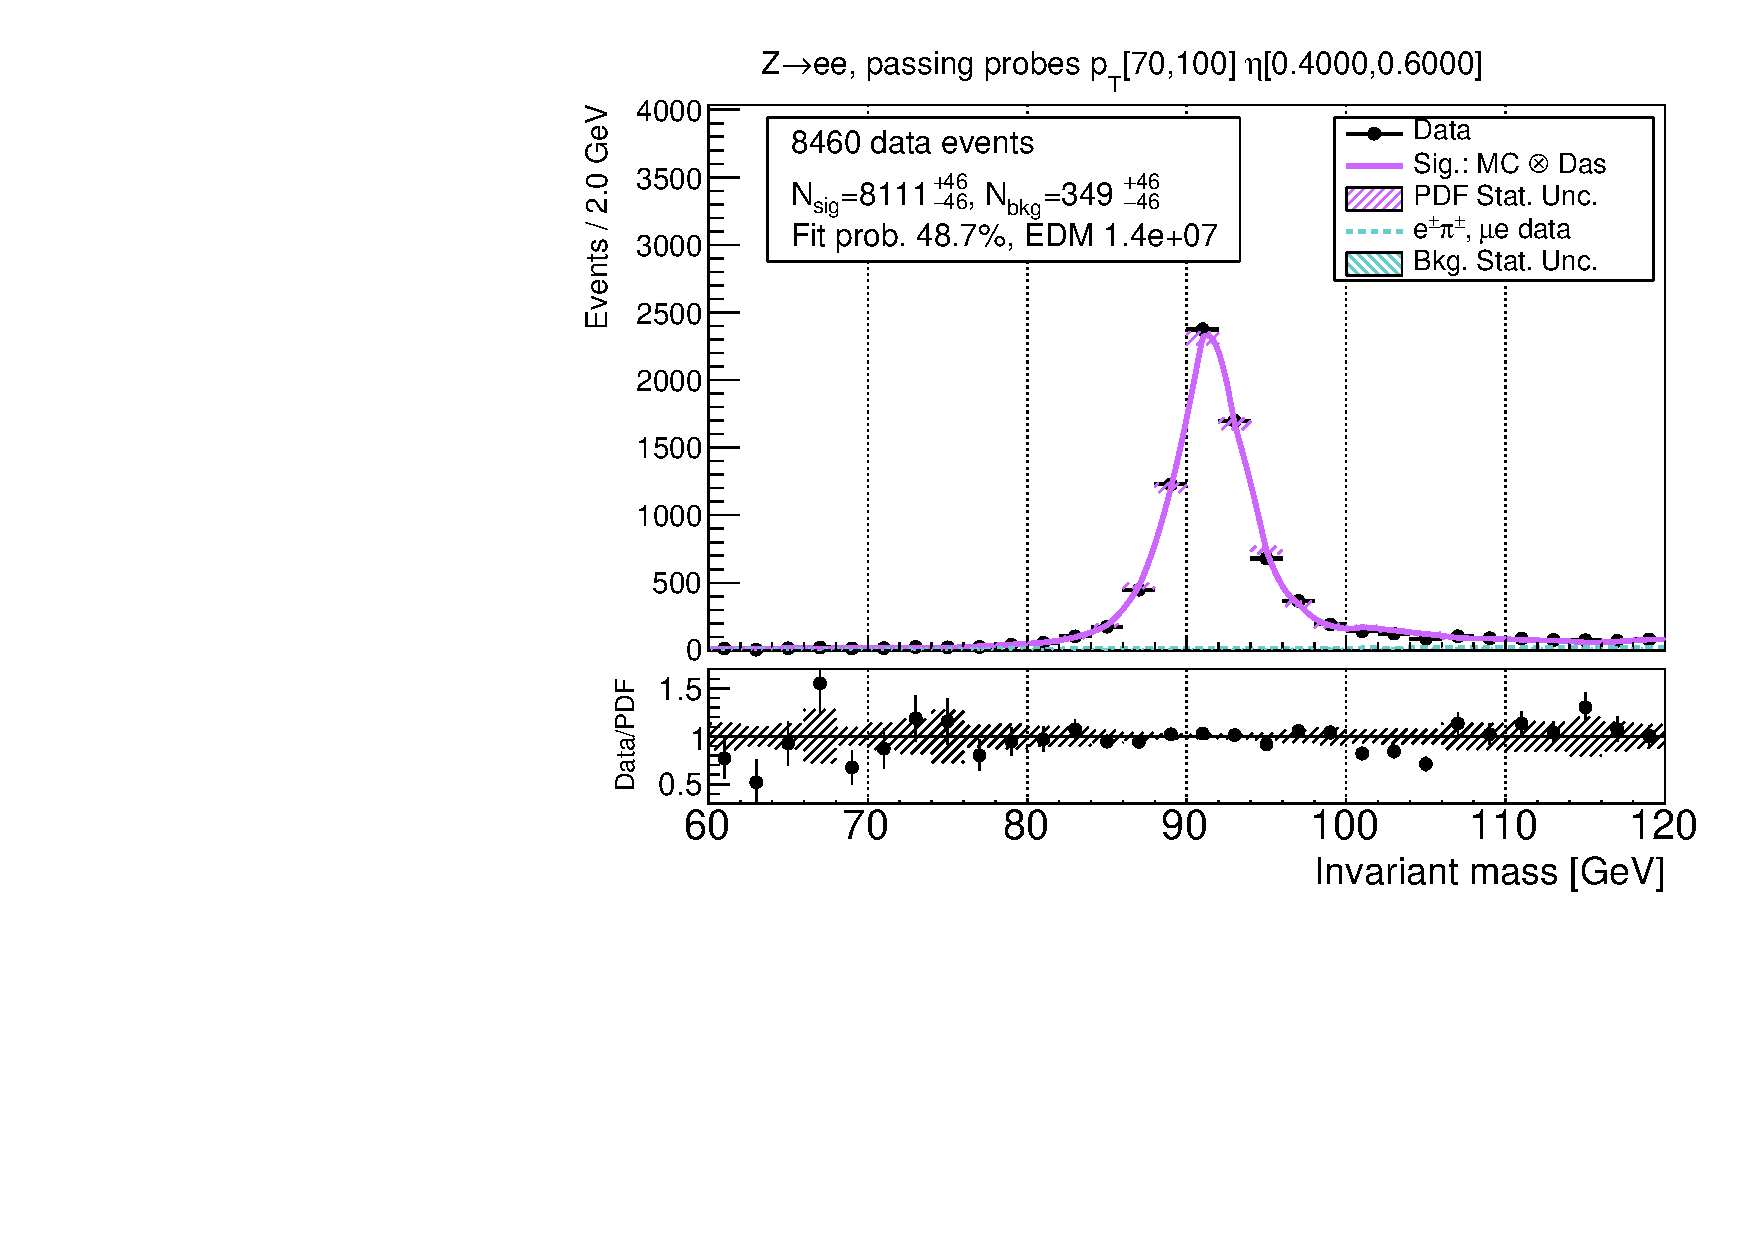
\includegraphics[width=0.49\textwidth]{figures/Zee_ResFunc_BkgLPiEMu_pass_ptBin14_etaBin17.pdf}
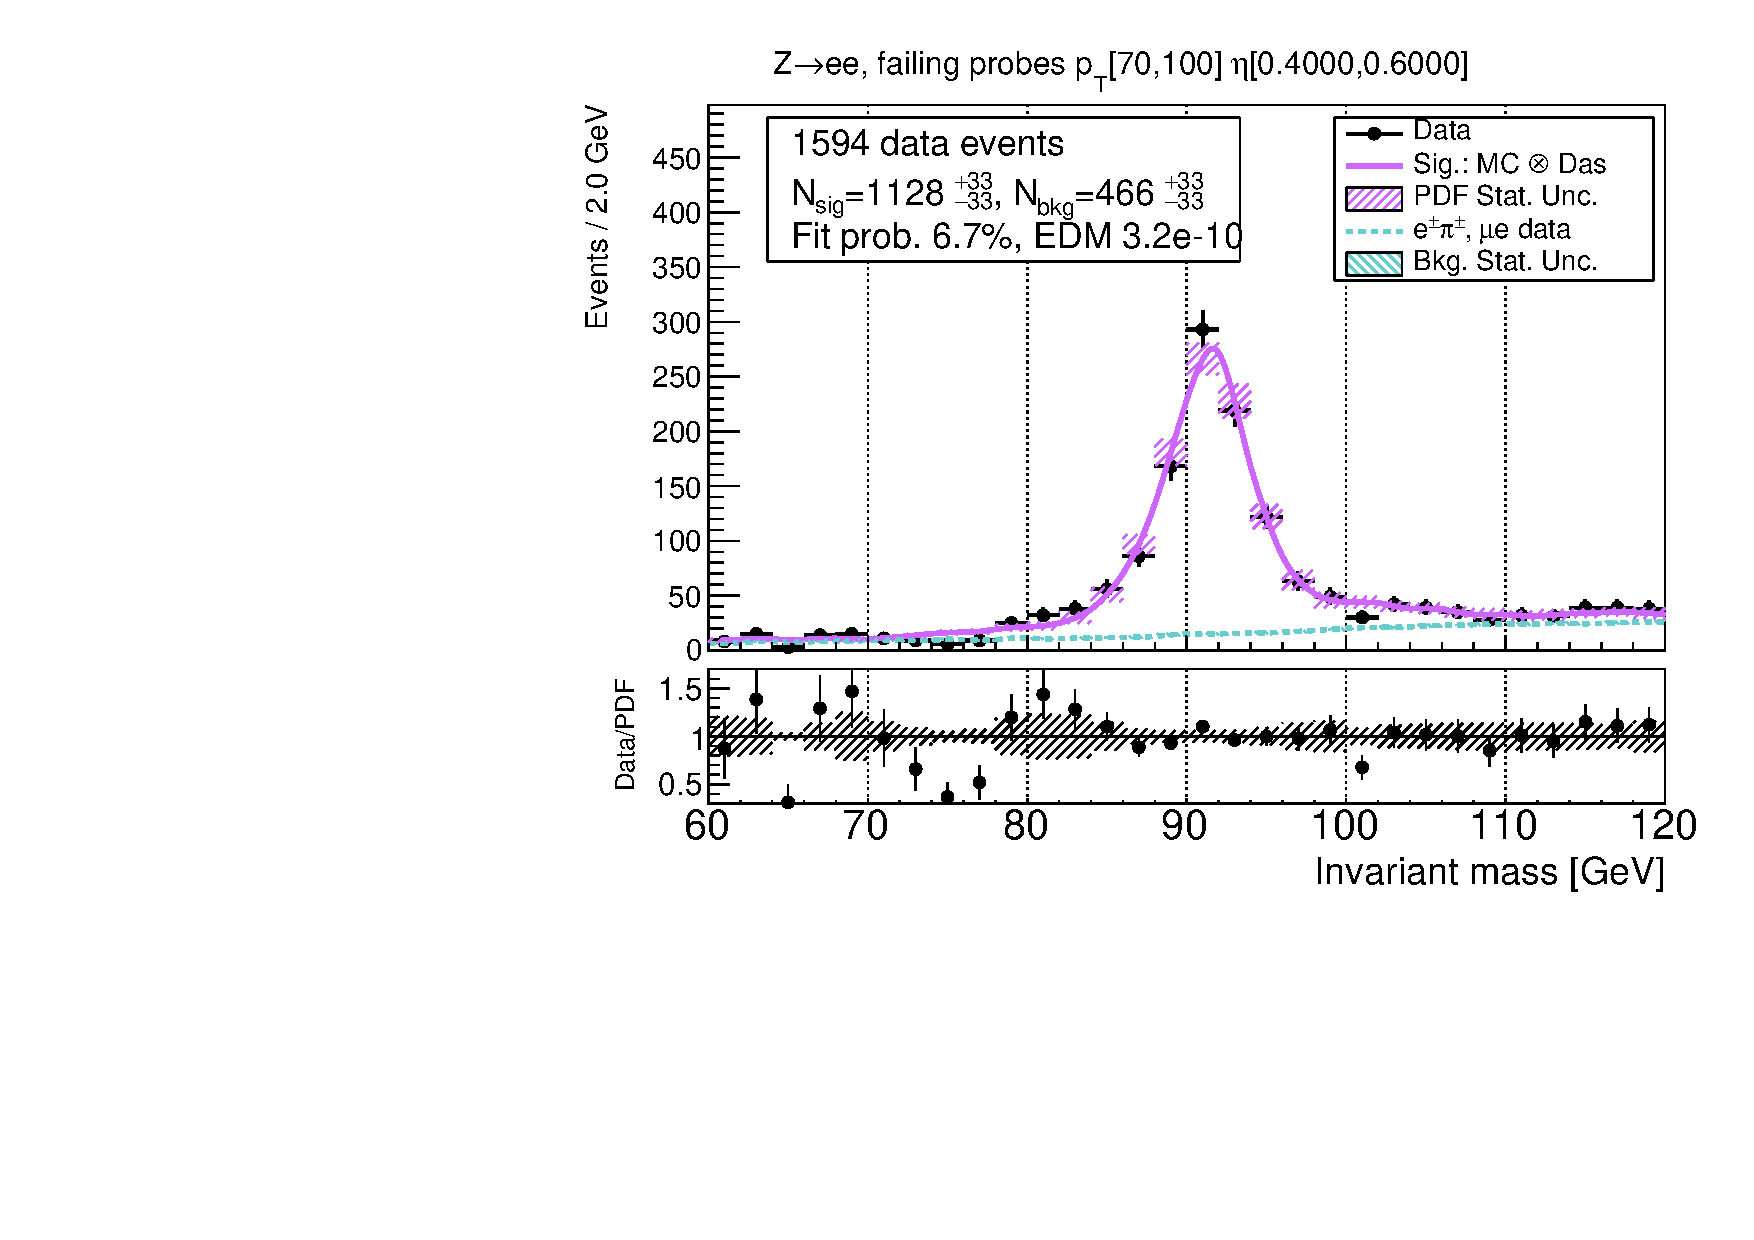
\includegraphics[width=0.49\textwidth]{figures/Zee_ResFunc_BkgLPiEMu_fail_ptBin14_etaBin17.pdf}
\caption{Efficiency extraction fits for the Medium electron working point using the analytic detector resolution function, at higher values of electron transverse momentum.}
\label{fig:ZeeAltSigResFits2}
\end{figure}


\clearpage
\subsection{Signal final state radiation modeling}
The reconstructed dilepton mass shape has a fat tail on the left side because of the effect of final state radiation (FSR).
In these tail events, at least one of the final state leptons radiates a photon,
reducing the energy of the dilepton system and changing the momentum of the emitting lepton.
It is more prevalent for electrons than for muons since bremsstrahlung is suppressed as the fourth power of lepton mass.

Simulation addresses the phenomenon of FSR well in Z boson reconstruction, but we must assess the uncertainty on
how FSR is modeled in the MC generator, which is only an approximation.
To do this, we consider an alternative showering program called PHOTOS. See Ref.~\cite{Golonka:2005pn}.
The goal is to compare the efficiencies obtained from fitting templates with different showering algorithm provenances.
Due to technical reasons, our NLO QCD generator of choice for the nominal fit model (aMC@NLO) could not be made to work with the PHOTOS showering algorithm.
Instead, we decided to use POWHEG then pursue a reweighting procedure to capture the effect.

First, we generated Monte Carlo events using POWHEG+PYTHIA8 (the nominal showering algorithm) and POWHEG+PHOTOS (the alternative showering algorithm).
In carrying out a private production only up to the GEN-SIM data tier, we were able to generate order of 10 million events for each showering choice.
Next, the events constituting the templates from the nominal generator were reweighted as a function of their generator-level mass 
to the corresponding distribution in the POWHEG+X samples, where X represents PYTHIA8 or PHOTOS. 
The generator-level mass is an appropriate variable for this procedure because radiated photons carrying off substantial energy, as modeled by the generator, will reduce the generator mass.
The altered weights were propagated to the histograms used as fitting templates, and fits were performed using the alternative POWHEG+X shapes.

Examples of these fits for 2016 run eras B to F are shown for dimuons in
Figures ~\ref{fig:ZmmAltSigFSRFits1},~\ref{fig:ZmmAltSigFSRFits2},~\ref{fig:ZmmAltSigFSRFits3}, and~\ref{fig:ZmmAltSigFSRFits4};
and for dielectrons in Figures~\ref{fig:ZeeAltSigFSRFits1},~\ref{fig:ZeeAltSigFSRFits2},~\ref{fig:ZeeAltSigFSRFits3}, and~\ref{fig:ZeeAltSigFSRFits4}.
These may be compared with the fits using the nominally simulated FSR tail.

To get alternative scale factors, the efficiencies extracted from data are divided by the respective cut-and-count Monte Carlo efficiency derived from the reweighted templates.
In other words, the data efficiency obtained by fitting with reweighted POWHEG+PYTHIA8 is divided by the cut-and-count MC efficiency from reweighted POWHEG+PYTHIA8, to get a scale factor.
Then, the systematic uncertainty in a kinematic bin is defined as the absolute difference between the POWHEG+X scale factors, in that bin:

\begin{equation}
%\begin{align*}
\delta_{\mathrm{FSR}} = \left| \frac{\varepsilon^{\mathrm{PYTHIA8}}_{\mathrm{Data}}}{\varepsilon^{\mathrm{PYTHIA8}}_{\mathrm{MC}}} - \frac{\varepsilon^{\mathrm{PHOTOS}}_{\mathrm{Data}}}{\varepsilon^{\mathrm{PHOTOS}}_{\mathrm{MC}}} \right|
%\end{align*}
\end{equation}

For 2D maps of the systematic uncertainty that results from this method, see Figures~\ref{fig:ZmmSystSigFSR} and~\ref{fig:ZeeSystSigFSR}.

\begin{figure}
\centering
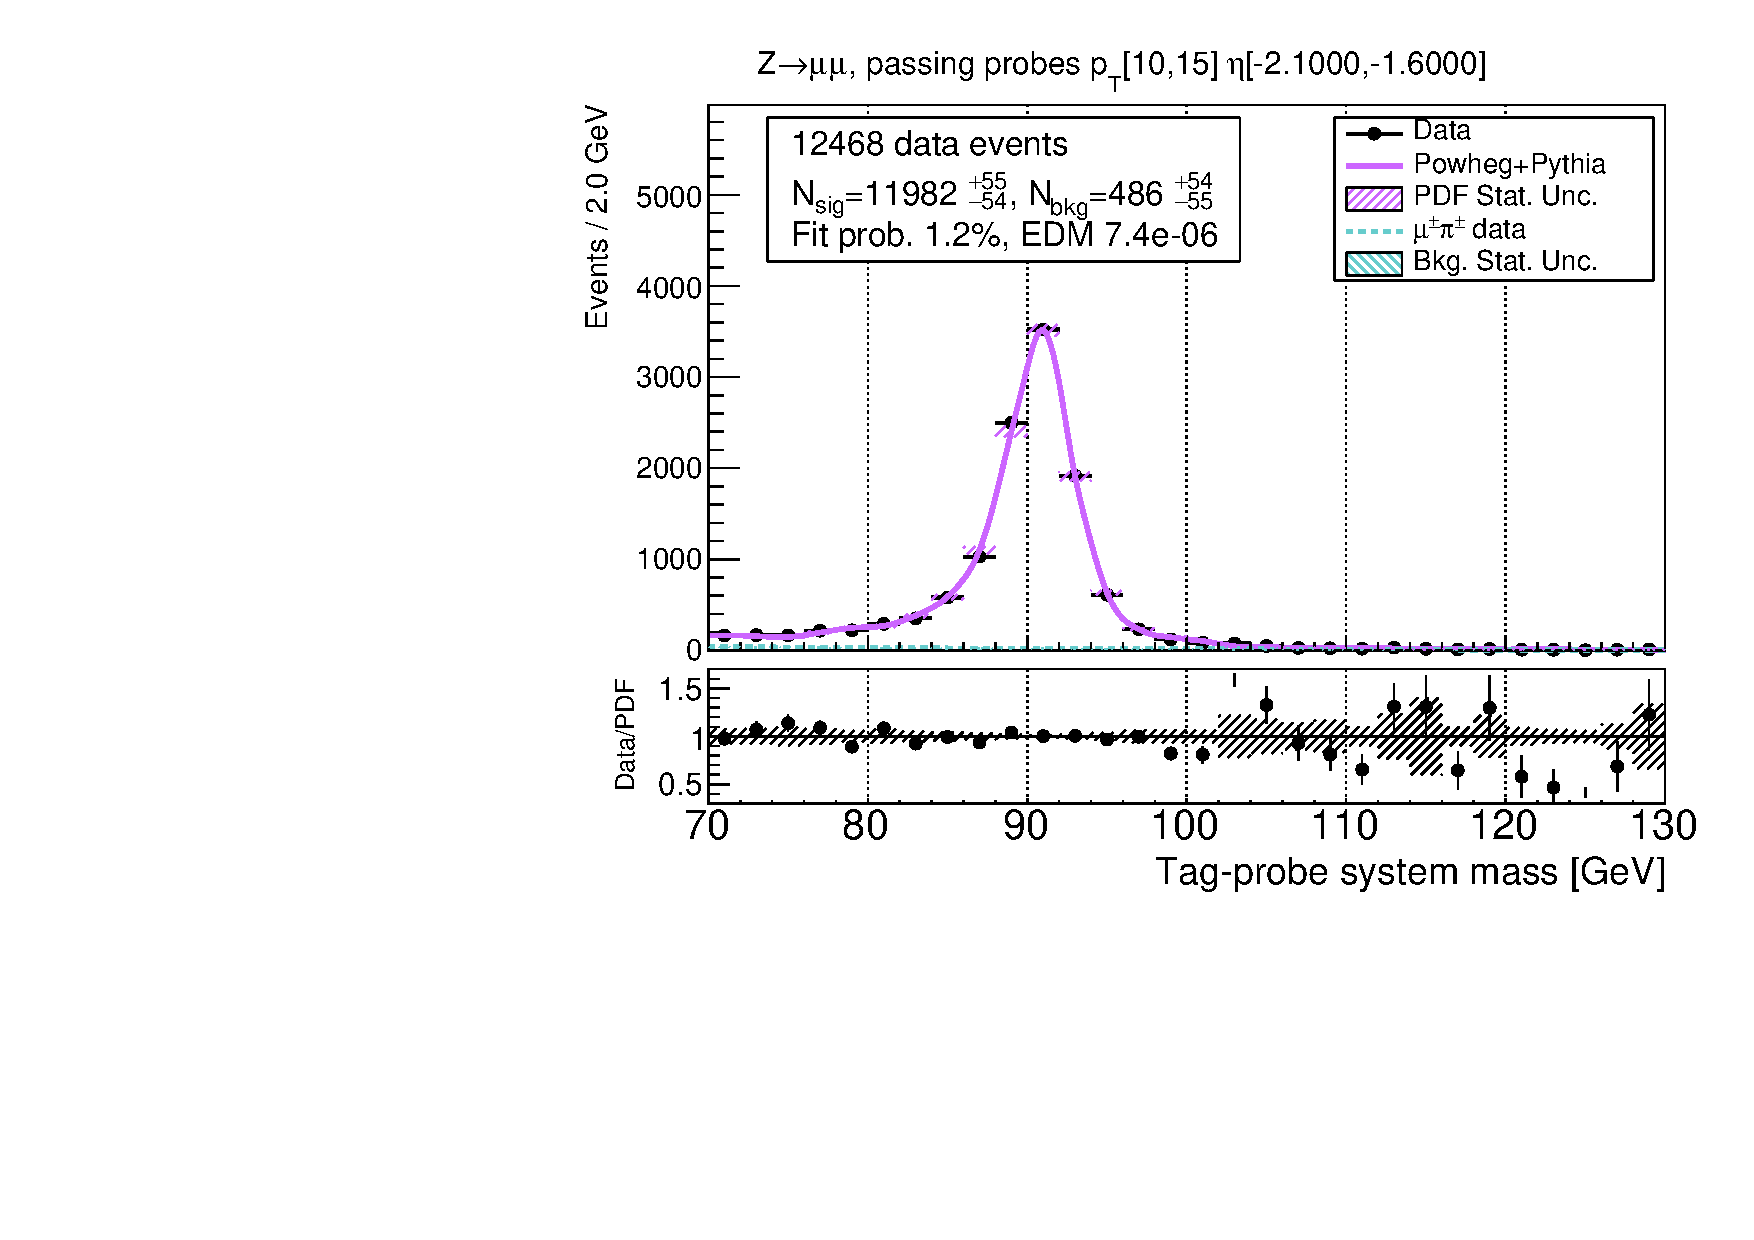
\includegraphics[width=0.49\textwidth]{figures/Zmm_PowhegPythia_BkgLPi_pass_ptBin0_etaBin1.pdf}
\includegraphics[width=0.49\textwidth]{figures/Zmm_PowhegPythia_BkgLPi_fail_ptBin0_etaBin1.pdf}
\includegraphics[width=0.49\textwidth]{figures/Zmm_PowhegPythia_BkgLPi_pass_ptBin1_etaBin9.pdf}
\includegraphics[width=0.49\textwidth]{figures/Zmm_PowhegPythia_BkgLPi_fail_ptBin1_etaBin9.pdf}
\caption{Efficiency extraction fits for the Medium muon working point using POWHEG and PYTHIA8, at low muon transverse momentum.}
\label{fig:ZmmAltSigFSRFits1}
\end{figure}
\begin{figure}
\centering
\includegraphics[width=0.49\textwidth]{figures/Zmm_PowhegPythia_BkgLPi_pass_ptBin7_etaBin0.pdf}
\includegraphics[width=0.49\textwidth]{figures/Zmm_PowhegPythia_BkgLPi_fail_ptBin7_etaBin0.pdf}
\includegraphics[width=0.49\textwidth]{figures/Zmm_PowhegPythia_BkgLPi_pass_ptBin10_etaBin6.pdf}
\includegraphics[width=0.49\textwidth]{figures/Zmm_PowhegPythia_BkgLPi_fail_ptBin10_etaBin6.pdf}
\caption{Efficiency extraction fits for the Medium muon working point using POWHEG and PYTHIA8, at higher values of muon transverse momentum.}
\label{fig:ZmmAltSigFSRFits2}
\end{figure}
\begin{figure}
\centering
\includegraphics[width=0.49\textwidth]{figures/Zmm_PowhegPhotos_BkgLPi_pass_ptBin0_etaBin1.pdf}
\includegraphics[width=0.49\textwidth]{figures/Zmm_PowhegPhotos_BkgLPi_fail_ptBin0_etaBin1.pdf}
\includegraphics[width=0.49\textwidth]{figures/Zmm_PowhegPhotos_BkgLPi_pass_ptBin1_etaBin9.pdf}
\includegraphics[width=0.49\textwidth]{figures/Zmm_PowhegPhotos_BkgLPi_fail_ptBin1_etaBin9.pdf}
\caption{Efficiency extraction fits for the Medium muon working point using POWHEG and PHOTOS, at low muon transverse momentum.}
\label{fig:ZmmAltSigFSRFits3}
\end{figure}
\begin{figure}
\centering
\includegraphics[width=0.49\textwidth]{figures/Zmm_PowhegPhotos_BkgLPi_pass_ptBin7_etaBin0.pdf}
\includegraphics[width=0.49\textwidth]{figures/Zmm_PowhegPhotos_BkgLPi_fail_ptBin7_etaBin0.pdf}
\includegraphics[width=0.49\textwidth]{figures/Zmm_PowhegPhotos_BkgLPi_pass_ptBin10_etaBin6.pdf}
\includegraphics[width=0.49\textwidth]{figures/Zmm_PowhegPhotos_BkgLPi_fail_ptBin10_etaBin6.pdf}
\caption{Efficiency extraction fits for the Medium muon working point using POWHEG and PHOTOS, at higher values of muon transverse momentum.}
\label{fig:ZmmAltSigFSRFits4}
\end{figure}

\begin{figure}
\centering
\includegraphics[width=0.49\textwidth]{figures/Zee_PowhegPythia_BkgLPiEMu_pass_ptBin0_etaBin0.pdf}
\includegraphics[width=0.49\textwidth]{figures/Zee_PowhegPythia_BkgLPiEMu_fail_ptBin0_etaBin0.pdf}
\includegraphics[width=0.49\textwidth]{figures/Zee_PowhegPythia_BkgLPiEMu_pass_ptBin1_etaBin19.pdf}
\includegraphics[width=0.49\textwidth]{figures/Zee_PowhegPythia_BkgLPiEMu_fail_ptBin1_etaBin19.pdf}
\caption{Efficiency extraction fits for the Medium electron working point using POWHEG and PYTHIA8, at low electron transverse momentum.}
\label{fig:ZeeAltSigFSRFits1}
\end{figure}
\begin{figure}
\centering
\includegraphics[width=0.49\textwidth]{figures/Zee_PowhegPythia_BkgLPiEMu_pass_ptBin3_etaBin23.pdf}
\includegraphics[width=0.49\textwidth]{figures/Zee_PowhegPythia_BkgLPiEMu_fail_ptBin3_etaBin23.pdf}
\includegraphics[width=0.49\textwidth]{figures/Zee_PowhegPythia_BkgLPiEMu_pass_ptBin14_etaBin17.pdf}
\includegraphics[width=0.49\textwidth]{figures/Zee_PowhegPythia_BkgLPiEMu_fail_ptBin14_etaBin17.pdf}
\caption{Efficiency extraction fits for the Medium electron working point using POWHEG and PYTHIA8, at higher values of electron transverse momentum.}
\label{fig:ZeeAltSigFSRFits2}
\end{figure}
\begin{figure}
\centering
\includegraphics[width=0.49\textwidth]{figures/Zee_PowhegPhotos_BkgLPiEMu_pass_ptBin0_etaBin0.pdf}
\includegraphics[width=0.49\textwidth]{figures/Zee_PowhegPhotos_BkgLPiEMu_fail_ptBin0_etaBin0.pdf}
\includegraphics[width=0.49\textwidth]{figures/Zee_PowhegPhotos_BkgLPiEMu_pass_ptBin1_etaBin19.pdf}
\includegraphics[width=0.49\textwidth]{figures/Zee_PowhegPhotos_BkgLPiEMu_fail_ptBin1_etaBin19.pdf}
\caption{Efficiency extraction fits for the Medium electron working point using POWHEG and PHOTOS, at low electron transverse momentum.}
\label{fig:ZeeAltSigFSRFits3}
\end{figure}

\begin{figure}
\centering
\includegraphics[width=0.49\textwidth]{figures/Zee_PowhegPhotos_BkgLPiEMu_pass_ptBin3_etaBin23.pdf}
\includegraphics[width=0.49\textwidth]{figures/Zee_PowhegPhotos_BkgLPiEMu_fail_ptBin3_etaBin23.pdf}
\includegraphics[width=0.49\textwidth]{figures/Zee_PowhegPhotos_BkgLPiEMu_pass_ptBin14_etaBin17.pdf}
\includegraphics[width=0.49\textwidth]{figures/Zee_PowhegPhotos_BkgLPiEMu_fail_ptBin14_etaBin17.pdf}
\caption{Efficiency extraction fits for the Medium electron working point using POWHEG and PHOTOS, at higher values of electron transverse momentum.}
\label{fig:ZeeAltSigFSRFits4}
\end{figure}


\clearpage
\subsection{Choice of generator}
The choice of generator used to determine the MC before the showering can affect the scale factor determination.
The differences in generator implementations, including leading-order versus next-to-leading order simulation,
can affect the fraction of passing and failing probes, and the truth-matching efficiency.
Therefore, we use a different implementation (\textsc{MadGraph5} at leading-order)
instead of the nominal (\textsc{MadGraph5\_aMC@NLO}) to extract the efficiency from data.
This data efficiency is divided by the nominal NLO MC efficiency to give an alternative scale factor. 
We do not substitute the leading-order MC efficiency here because, 
for the purposes of a precision measurement, the difference in the data efficiency is the real effect.
We take the size of the difference in the scale factors as the symmetric systematic uncertainty from the choice of generator.
See Figures~\ref{fig:ZmmSystMCGen} and~\ref{fig:ZeeSystMCGen}.


\clearpage
\subsection{Bias from choice of tag selection}
The choice of tag selection cuts is motivated by the realities of the experiment, such as
detector acceptance and trigger $p_{T}$ thresholds. The tag selection can bias the data efficiency,
so we account for this by observing the change in the Data/MC scale factors when the 
tag selection is changed. The alternative tag selection has a $p_{T}$ threshold 5 $\GeV$ higher, and 
uses the Medium working point for identification and isolation.

Examples of fits for 2016 run eras B to F with the alternative tag selection applied to Data and MC are shown for dimuons in
Figures ~\ref{fig:ZmmAltAltTagFits1} and~\ref{fig:ZmmAltAltTagFits2}, 
and for dielectrons in Figures~\ref{fig:ZeeAltAltTagFits1} and~\ref{fig:ZeeAltAltTagFits2}.
These may be compared with the fits using the nominal tag selection in section \ref{sec:tnpfits}.
The difference in the Data/MC scale factors derived using the two methods is taken as a systematic; 
see Figures~\ref{fig:ZmmSystAltTag} and~\ref{fig:ZeeSystAltTag}.

\begin{figure}
\centering
\includegraphics[width=0.49\textwidth]{figures/Zmm_AltTag_pass_ptBin0_etaBin1.pdf}
\includegraphics[width=0.49\textwidth]{figures/Zmm_AltTag_fail_ptBin0_etaBin1.pdf}
\includegraphics[width=0.49\textwidth]{figures/Zmm_AltTag_pass_ptBin1_etaBin9.pdf}
\includegraphics[width=0.49\textwidth]{figures/Zmm_AltTag_fail_ptBin1_etaBin9.pdf}
\caption{Efficiency extraction fits for the Medium muon working point using the alternative tag selection, at low muon transverse momentum.}
\label{fig:ZmmAltAltTagFits1}
\end{figure}

\begin{figure}
\centering
\includegraphics[width=0.49\textwidth]{figures/Zmm_AltTag_pass_ptBin7_etaBin0.pdf}
\includegraphics[width=0.49\textwidth]{figures/Zmm_AltTag_fail_ptBin7_etaBin0.pdf}
\includegraphics[width=0.49\textwidth]{figures/Zmm_AltTag_pass_ptBin10_etaBin6.pdf}
\includegraphics[width=0.49\textwidth]{figures/Zmm_AltTag_fail_ptBin10_etaBin6.pdf}
\caption{Efficiency extraction fits for the Medium muon working point using the alternative tag selection, at higher values of muon transverse momentum.}
\label{fig:ZmmAltAltTagFits2}
\end{figure}

\begin{figure}
\centering
\includegraphics[width=0.49\textwidth]{figures/Zee_AltTag_pass_ptBin0_etaBin0.pdf}
\includegraphics[width=0.49\textwidth]{figures/Zee_AltTag_fail_ptBin0_etaBin0.pdf}
\includegraphics[width=0.49\textwidth]{figures/Zee_AltTag_pass_ptBin1_etaBin19.pdf}
\includegraphics[width=0.49\textwidth]{figures/Zee_AltTag_fail_ptBin1_etaBin19.pdf}
\caption{Efficiency extraction fits for the Medium electron working point using the alternative tag selection, at low electron transverse momentum.}
\label{fig:ZeeAltAltTagFits1}
\end{figure}

\begin{figure}
\centering
\includegraphics[width=0.49\textwidth]{figures/Zee_AltTag_pass_ptBin3_etaBin23.pdf}
\includegraphics[width=0.49\textwidth]{figures/Zee_AltTag_fail_ptBin3_etaBin23.pdf}
\includegraphics[width=0.49\textwidth]{figures/Zee_AltTag_pass_ptBin14_etaBin17.pdf}
\includegraphics[width=0.49\textwidth]{figures/Zee_AltTag_fail_ptBin14_etaBin17.pdf}
\caption{Efficiency extraction fits for the Medium electron working point using the alternative tag selection, at higher values of electron transverse momentum.}
\label{fig:ZeeAltAltTagFits2}
\end{figure}

\clearpage

\subsection{Total impact of systematic uncertainties}
The percent impacts of each source of uncertainty on the inclusive Z($\ellell$) cross section
are shown in Table~\ref{tab:ZYieldImpacts}. Pre-HIP mitigation scenario in 2016 is assumed.

\begin{table}[htbp]
  \begin{center}
 {\small
  \begin{tabular} {lrr}
\hline
  \multirow{2}{*}{Source of Uncertainty} & Z(ee) Yield& Z($\mu\mu$) Yield \\
                                         & \% Impact  & \% Impact         \\
  \hline
  Background shape                       & 0.48       & 0.57              \\
  Signal resolution                      & 0.04       & 0.26              \\
  Signal FSR model                       & 0.09       & 0.07              \\
  Generator choice                       & 0.34       & 0.19              \\
  Tag selection                          & 0.44       & 0.26              \\
  \hline                                                           
  Total scale factor impact              & 0.74       & 0.71              \\
  \hline
  \end{tabular}
}
  \caption{Impact of the scale factor uncertainties on the inclusive cross section.}
  \label{tab:ZYieldImpacts}
  \end{center}
\end{table}


